\documentclass[12pt, a4paper, twoside]{report}
\usepackage{amsmath, amssymb}
\usepackage{geometry}
\usepackage{fancyhdr}
\usepackage{graphicx}
\usepackage{titlesec}
\usepackage{fontspec}
\usepackage{tocloft} 
\usepackage{natbib}
\usepackage{float}
\usepackage{colortbl}
\usepackage{enumitem}
\usepackage[table]{xcolor}

\graphicspath{ {./images/} }

% Page settings
\geometry{
    a4paper,
    top=5cm,
    bottom=4.8cm,
    left=3.7cm,
    right=3.7cm,
    headheight=4.3cm, % Header height set to 4.3 cm
     headsep=0.5cm, % Adjust this value if needed to control spacing between header and text
    footskip=0cm % No extra space for footer
}


\definecolor{lightgreen}{rgb}{0.82, 0.94, 0.75}
\definecolor{lightorange}{rgb}{0.98, 0.84, 0.65}
\newcolumntype{L}{>{\centering\arraybackslash}m{10cm}}
\newcolumntype{l}{>{\centering\arraybackslash}m{7cm}}
\def\BibTeX{{\rm B\kern-.05em{\sc i\kern-.025em b}\kern-.08em
    T\kern-.1667em\lower.7ex\hbox{E}\kern-.125emX}}

\setlist[itemize]{itemsep=0pt, topsep=0pt, parsep=0pt, partopsep=0pt}

% Font settings
\setmainfont{Verdana}
\newfontface\symbolsfont{Symbol} % For unsupported mathematical symbols

% Title and section fonts with sizes
\titleformat{\chapter}[hang]{\fontsize{14pt}{14pt}\selectfont\bfseries}{\thechapter.}{20pt}{\fontsize{14pt}{14pt}\selectfont\bfseries}
\titleformat{\section}[hang]{\fontsize{11pt}{11pt}\selectfont\bfseries}{\thesection.}{12pt}{\fontsize{11pt}{11pt}\selectfont\bfseries}
\titleformat{\subsection}[hang]{\fontsize{10pt}{10pt}\selectfont\bfseries}{\thesubsection.}{10pt}{\fontsize{10pt}{10pt}\selectfont\bfseries}


% Paragraph indent and spacing
\setlength{\parindent}{1.27cm} % Tabs equivalent to 1.27 cm
\setlength{\parskip}{9pt} % Spacing between paragraphs
% Fancy header settings

\pagestyle{fancy}
\fancyhf{} % Clear all header and footer fields

% Header settings

\fancyhead[RO]{\fontsize{9pt}{11pt}\selectfont  \thechapter \hspace{0.1em} - \hspace{0.1em} \rightmark \hspace{1em} \thepage}  % Odd pages: Section title on the right, then page number
\fancyhead[LE]{\fontsize{9pt}{11pt}\selectfont \thepage \hspace{1em} \leftmark \hspace{0.1em} - \hspace{0.1em} \thechapter}  % \thesection Even pages: Page number on the left, then chapter title

\renewcommand{\chaptermark}[1]{\markboth{#1}{}} % Only chapter title in the header
\renewcommand{\sectionmark}[1]{\markright{#1}}

\fancypagestyle{plain}{
    \fancyhf{} % Clear all header and footer fields for chapter start pages
    \renewcommand{\headrulewidth}{0pt} % Remove header line
    \renewcommand{\footrulewidth}{0pt} % Remove footer line
}

% TOC, List of Figures, and List of Tables Customizations

% Suppress the default ToC, LoF, LoT titles by making them empty
\renewcommand{\contentsname}{}
\renewcommand{\listfigurename}{}
\renewcommand{\listtablename}{}

% Manually insert a centered, bold, uppercase title in the respective pages
\addtocontents{toc}{\protect\begin{center}\MakeUppercase{\bfseries\fontsize{9pt}{14pt}\selectfont Contents}\protect\end{center}\vspace*{-1em}\vspace{1\baselineskip}}
\addtocontents{lof}{\protect\begin{center}\MakeUppercase{\bfseries\fontsize{9pt}{14pt}\selectfont List of Figures}\protect\end{center}\vspace*{-1em}\vspace{1\baselineskip}}
\addtocontents{lot}{\protect\begin{center}\MakeUppercase{\bfseries\fontsize{9pt}{14pt}\selectfont List of Tables}\protect\end{center}\vspace*{-1em}\vspace{1\baselineskip}}

% Ensure entries in the Table of Contents, List of Figures, and List of Tables are in normal font
\renewcommand{\cftchapfont}{\normalfont\fontsize{9pt}{11pt}\selectfont} % Chapter entries in normal font
\renewcommand{\cftsecfont}{\normalfont\fontsize{9pt}{11pt}\selectfont} % Section entries in normal font
\renewcommand{\cftsubsecfont}{\normalfont\fontsize{9pt}{11pt}\selectfont} % Subsection entries in normal font
\renewcommand{\cftchappagefont}{\normalfont\fontsize{9pt}{11pt}\selectfont} % Page numbers for chapters in normal font
\renewcommand{\cftsecpagefont}{\normalfont\fontsize{9pt}{11pt}\selectfont} % Page numbers for sections in normal font
\renewcommand{\cftsubsecpagefont}{\normalfont\fontsize{9pt}{11pt}\selectfont} % Page numbers for subsections in normal font
\renewcommand{\cftdotsep}{1} % Set dot separation for entries to be closer together


% Title and section fonts with sizes
\titleformat{\chapter}[block]
  {\centering\normalfont\fontsize{14pt}{14pt}\selectfont\bfseries}
  {\thechapter.} 
  {0.5em} 
  {\MakeUppercase} 
  [\vspace{0pt}] 

% Spacing before and after chapters and sections to control vertical positioning
\titlespacing*{\chapter}{1.27cm}{3pt}{18pt} % 3 spaces of 9pt before chapter, 2 spaces of 9pt after chapter title
\titlespacing*{\section}{1.27cm}{18pt}{9pt} % 2 spaces of 9pt before section, 1 space of 9pt after section title
\titlespacing*{\subsection}{1.27cm}{9pt}{9pt} % 1 space of 9pt before and after subsection


% Adjust Table of Contents Layout


\setlength{\cftchapindent}{0pt} % No indent for chapters
\setlength{\cftsecindent}{1.5em} % Set indent for sections
\setlength{\cftsubsecindent}{3em} % Set indent for subsections
\setlength{\cftsubsubsecindent}{4.5em} 

\setlength{\cftchapnumwidth}{2em} % Set space for chapter numbers
\setlength{\cftsecnumwidth}{3em}  % Set space for section numbers
\setlength{\cftsubsecnumwidth}{4em} % Set space for subsection numbers

\let\origaddcontentsline\addcontentsline
\renewcommand{\addcontentsline}[3]{\origaddcontentsline{#1}{#2}{\numberline{}#3}}

\setlength{\cftbeforechapskip}{0pt}

\renewcommand{\normalsize}{\fontsize{9pt}{11pt}\selectfont}
\normalsize 

\def\BibTeX{{\rm B\kern-.05em{\sc i\kern-.025em b}\kern-.08em
    T\kern-.1667em\lower.7ex\hbox{E}\kern-.125emX}}

\newcommand*{\Comb}[2]{{}^{#1}C_{#2}}%

\begin{document}
\vspace*{-4cm}
\pagestyle{empty}
\tableofcontents
\clearpage

\newpage
\vspace*{-4cm}
\listoftables

\newpage
\vspace*{-4cm}
\listoffigures


\pagestyle{fancy}


\newpage
\chapter{Introduction}
\section{Research scope and motivation}


The domain of the proposed thesis is Automated Software Engineering. The thesis will develop methods for the analysis of legacy software systems, focusing on using historical information describing the evolution of the systems extracted from the versioning systems. 
The methods for analysis will integrate techniques based on computational algorithms as well as data-mining. As proof-of-concept, tool prototypes will implement the proposed methods and validate them by extensive experimentation on several cases of real-life systems.\\

\section{Objectives of the thesis}

\section{Structure of the thesis}

\section{Main Contributions}



\chapter{State of the art in software dependencies}
\label{dep}


\section{Structural dependencies}
A dependency is created by two elements that are in a relationship and indicates that an element of the relationship, in some manner, depends on the other element of the relationship \cite{Booch:2004:OAD:975416}, \cite{Cataldo2009SoftwareDW}.

Structural dependencies can be found by analyzing the source code \cite{Sangal:2005:UDM:1094811.1094824}, \cite{CalloArias2011}. 
There are several types of relationships between these source code entities and all those create \textit{structural dependencies}:

\subsubsection{Data Item Dependencies}
Data items can be variables, records or structures. A dependency is created between two data items when the value held in the first data item is used or affects the value from the second.

\subsubsection{Data Type Dependencies}
Data items are declared to be of a specific data type. Besides the built-in data types that every programming language has, developers can also create new types that they can use. Each time the data type definition is changed it will affect all the data items that are declared to be of that type. 

\subsubsection{Subprogram Dependencies}
A subprogram is a sequence of instructions that performs a certain task. Depending on the programming language a subprogram may also be called a routine, a method, a function or a procedure. When a subprogram is changed, the developer must check the effects of that change in all the places that are calling that subprogram. Subprograms may also have dependencies with the data items that they receive as input or the data items that they are computing.



\section{Logical dependencies}

\subsection{Software change}
\label{change}

Software has distinctive stages during its life: Initial development, Evolution, Servicing, Phase out and Close down \cite{Software-life-cycle}, \cite{model-bennett}.

In the \textit{evolution stage} iterative changes are made. By changes, we mean additions (new software features), modifications (changes of requirements or misunderstood requirements) or deletions. There are two main reasons for the change: the learning process of the software team and new requests from the client.

If new changes are no longer easy to be made or are very difficult and time-consuming, the software enters the \textit{servicing stage} also called aging software, decayed software and legacy \cite{Software-life-cycle}, \cite{363157}.

The main difference between changes made in the evolution stage and changes made in the servicing stage is the effort of making changes. In the evolution stage, software changes are made easily and do not require much effort while in the servicing stage only a limited number of changes are made and require a lot of effort, so are really time-consuming \cite{Bennett}, \cite{Rajlich}.

The change mini-cycle consists of the following phases \cite{810308}:
\begin{itemize}
\item Phase 1: The request for change. This usually comes from the users of the software and it can also be a bug report or a request for an additional functionality. 
\item Phase 2: The planning phase, this includes program comprehension and change impact analysis. Program comprehension is a mandatory prerequisite of the change while change
impact analysis indicates how costly the change is going to be. \cite{Bohner}
\item Phase 3: The change implementation, restructuring for change and change propagation.
\item Phase 4: Verification and validation.
\item Phase 5: Re-documentation.
\end{itemize}


\subsection{Version control systems}

Software evolution implies change which can be triggered either by new feature requests or bug reports \cite{articleEvolution}. As presented also in section \ref{change}, one phase of the change mini-cycle consists of change implementation and propagation (changing source code files). 
Usually, developers use version control when it comes to software development. Version control is a system that records changes to a file or set of files over time so that developers can recall specific versions of those files later \cite{svn}.
Distributed version control systems (such as Git, Mercurial, Bazaar or Darcs) allows many developers to collaboratively develop their projects \cite{7471284}.

\subsection{Logical dedependencies in software systems}
\textit{Logical dependencies} (a.k.a logical coupling) can be found by software history analysis and can reveal relationships that are not always present in the source code (structural dependencies).  

Software engineering practice has shown that sometimes modules which do not present structural dependencies still appear to be related. Co-evolution represents the phenomenon when one component changes in response to a change in another component \cite{Yu:2007:UCC:1231330.1231370}, \cite{5166450}. Those changes can be found in the software history maintained by the versioning system. Gall \cite{Gall:1998:DLC:850947.853338}, \cite{Gall:2003:CRH:942803.943741} identified as logical coupling between two modules the fact that these modules  \textit{repeatedly} change together during the historical evolution of the software system \cite{6606615}.

The concepts of logical coupling and logical dependencies were first used in different analysis tasks, all related to changes: for software change impact analysis \cite{1553643}, for identifying the potential ripple effects caused by software changes during software maintenance and evolution \cite{DBLP:conf/issre/OlivaG15}, \cite{Oliva:2011:ISL:2067853.2068086}, \cite{Poshyvanyk2009}, \cite{posh2010} or for their link to deffects \cite{wiese}, \cite{Zimmermann:2004:MVH:998675.999460}.

The current trend recommends that general dependency management methods and tools should also include logical dependencies besides the structural dependencies \cite{Oliva:2011:ISL:2067853.2068086}, \cite{DBLP:journals/jss/AjienkaC17}. 


\subsection{Current status of research}

Oliva and Gerosa \cite{Oliva:2011:ISL:2067853.2068086}, \cite{DBLP:conf/issre/OlivaG15} have found first that the set of co-changed classes was much larger compared to the set of structurally coupled classes. They identified structural and logical dependencies from 150000 revisions from the Apache Software Foundation SVN repository. Also they concluded  that in at least 91\% of the cases, logical dependencies involve files that are not structurally related. This implies that not all of the change dependencies are related to structural dependencies and there could be other reasons for software artifacts to be change dependent.

Ajienka and Capiluppi also studied the interplay between logical and structural coupling of software classes. In \cite{DBLP:journals/jss/AjienkaC17} they  perform experiments on 79 open source systems: for each system, they determine the sets of structural dependencies, the set of logical dependencies and the intersections of these sets. They quantify the overlapping or intersection of these sets, coming to the conclusion that not all co-changed class pairs (classes with logical dependencies) are also linked by structural dependencies. One other interesting aspect which has not been investigated by the authors in \cite{DBLP:journals/jss/AjienkaC17}  is the total number of logical dependencies, reported to the total number of structural dependencies of a software systems. However, they provide the raw data of their measurements and we calculated the ratio between the number of logical dependencies and the number of structural dependencies for all the projects analyzed by them: the average ratio resulted 12.  This means that, using their method of detecting logical dependencies for a system, the number of logical dependencies outnumbers by one order of magnitude the number of structural dependencies. We consider that such a big number of logical dependencies needs additional filtering. 


Another kind of non-structural dependencies are the semantic or conceptual dependencies \cite{Poshyvanyk2009}, \cite{posh2010}. Semantic coupling is given by the degree to which the identifiers and comments from different classes are similar to each other. Semantic coupling could be an indicator for logical dependencies, as studied by Ajienka et al in \cite{DBLP:journals/ese/AjienkaCC18}. The experiments showed that a large number of co-evolving classes do not present semantic coupling, adding to the earlier research which showed that a large number of co-evolving classes do not present structural coupling. All these experimental findings rise the question whether it is a legitimate approach to accept all co-evolving classes as logical coupling.

Zimmermann et al \cite{Zimmermann:2004:MVH:998675.999460} introduced data mining techniques to obtain association rules from version histories.
The mined association rules  have a probabilistic interpretation based on the amount of evidence in the transactions they are derived from. This amount of evidence is determined by two measures: support and confidence.  They developed a tool to predict future or missing changes.

Different applications based on dependency analysis could be improved if, beyond structural dependencies, they also take into account the hidden non-structural dependencies. For example, works  which investigate different methods for architectural reconstruction \cite{SoraConti}, \cite{SoraSem13}, \cite{PagerankENASE},  all of them based on the information provided by structural dependencies, could enrich their dependency models by taking into account also logical dependencies. However, a thorough survey \cite{sar} shows that historical information has been rarely used in architectural reconstruction. 

Another survey \cite{Shtern:2012:CMS:2332427.2332428} mentions one possible explanation why historical information have been rarely used in architectural reconstruction: the size of the extracted information. One problem is the size of the extraction process, which has to analyze many versions from the historical evolution of the system. Another problem is the big number of pairs of classes which record co-changes and how they relate to the number of pairs of classes with structural dependencies.

The software architecture is important in order to understand and maintain a system. Often code updates are made without checking or updating the architecture. This kind of updates cause the architecture to drift from the reality of the code over time \cite{sar}.
So reconstructing the architecture and verifying if still matches the reality is important \cite{Kalliamvakou2016}. 

Surveys also show that architectural reconstruction is mainly made based on structural dependencies \cite{Shtern:2012:CMS:2332427.2332428}, \cite{sar}, the main reason why historical information is rarely used in architectural reconstruction is the size of the extracted information.

Logical dependencies should integrate harmoniously with structural dependencies in an unitary dependency model: valid logical dependencies should not be omitted from the dependency model, but structural dependencies should not be engulfed by questionable logical dependencies generated by casual co-changes.  
Thus, in order to add logical dependencies besides structural dependencies in dependency models, class co-changes must be filtered until they remain only a reduced but relevant set of valid logical dependencies. 

Currently there is no set of rules or best practices that can be applied to the extracted class co-changes and can guarantee their filtering into a set of valid logical dependencies.
This is mainly because not all the updates made in the versioning system are code related. For example a commit that has as participants a big number of files can indicate that a merge with another branch or a folder renaming has been made. In this case, a series of irrelevant co-changing pairs of entities can be introduced. So, in order to exclude this kind of situations the information extracted from the versioning system has to be filtered first and then used.

Other works have tried to filter co-changes \cite{Oliva:2011:ISL:2067853.2068086}, \cite{DBLP:journals/jss/AjienkaC17}. One of the used co-changes filter is the commit size.The commit size is the number of code files changed in that particular commit. 
Ajienka and Capiluppi established a threshold of 10 for the maximum accepted size for a commit \cite{DBLP:journals/jss/AjienkaC17}. This means that all the commits that had more than 10 code files changed where discarded from the research. But setting a harcoded threshold for the commit size is debatable because in order to say that a commit is big or small you have to look first at the size of the system and at the trends from the versioning system. Even thought the best practices encourage small and often commits, the developers culture is the one that influences the most the trending size of commits from one system.

Filtering only after commit size is not enough, this type of filtering can indeed have an impact on the total number of extracted co-changes, but will only shrink the number of co-changes extracted without actually guaranteeing that the remaining ones have more relevancy and are more logical linked.

Although, some unrelated files can be updated by human error in small commits, for example: one file was forgot to be commited in the current commit and will be commited in the next one among some unrelated files. This kind of situation can introduce a set of co-changing pairs that are definitely not logical liked. In order to avoid this kind of situation a filter for the occurrence rate of co-changing pairs must be introduced. Co-changing pairs that occur multiple times are more prone to be logically dependent than the ones that occur only once. Currently there are no concrete examples of how the threshold for this type of filter can be calculated. In order to do that, incrementing the threshold by a certain step will be the start and then studying the impact on the remaining co-changing pairs for different systems. 

Taking into account also structural dependencies from all the revisions of the system was not made in previous works, this step is important in order to filter out the old, out-of-date logical dependencies. Some logical dependencies may have been also structural in previous revisions of the system but not in the current one. If we take into consideration also structural dependencies from previous revisions then the overlapping rate between logical and structural dependencies could probably increase. Another way to investigate this problem could be to study the trend of concurrences of co-changes: if co-changes between a pair of classes used to happen more often in the remote past than in the more recent past, it may be a sign that the problem causing the logical coupling has been removed in the mean time. 


\section{Applications of software dependencies}
\label{app}

\subsection{Reverse engineering}
The term reverse engineering was first defined by Chikofsky and Cross \cite{ChikofskyReverse} as the \textit{"process of analyzing a system to (i) identify the system’s components and
their inter-relationships and (ii) create representations of the system in another form or at a higher level of abstraction."} 

Reverse engineering is viewed as a two step process: information extraction and abstraction. \cite{FoSEReverseEngineering} 
The firs step, information extraction, is made by source code analysis which generates dependencies between software artifacts. So, reverse engineering uses dependencies in order to create new representations of the system or provide a higher level of abstraction \cite{struct_dep}, \cite{Gueheneuc}.

\subsection{Architecture reconstruction}
Currently, the software systems contain tens of thousands of lines of code and are updated multiple times a day by multiple developers.  
The software architecture is important in order to understand and maintain a system. Often code updates are made without checking or updating the architecture.
This kind of updates cause the architecture to drift from the reality of the code over time. So reconstructing the architecture and verifying if still matches the reality is important. \cite{sar},\cite{PagerankENASE}, \cite{Bass-archreconstruction} ,\cite{RecoverySartipi}, \cite{model-bennett}.

\subsection{Identifying clones}
Research suggests that a considerable part (around 5-10\%) of the source code of large-scale software is duplicate code (“clones”). Source code is often duplicated for a variety of reasons, programmers may simply be reusing a piece of code by copy and paste or they may be “reinventing the wheel” \cite{ClonesMayrand}, \cite{clones}.
Detection and removal of clones can decrease software maintenance costs \cite{CloneDetection}, \cite{cloneKamiya}.

\subsection{Code smells }
Code smells have been defined by Fowler \cite{bookFowler} and describe patterns that are generally associated with bad design and bad programming practices.
Originally, code smells are used to find the places in software may need refactoring \cite{articlesmells}. Studies have found that smells may affect comprehension and possibly increase change and fault proneness \cite{5741260}, \cite{5328703}, \cite{articlefault-proneness}.
Examples of code smells:
\begin{itemize}
	\item Large Class: one class with many fields.
	\item Feature Envy:  methods that access more methods and fields of another class than of its own class.
	\item Data Class: classes that only fields and do not contain functionality.
	\item Refused Bequest: classes that leave many of the fields and methods they inherit unused
	\item Parallel Inheritance: every time you make a subclass of one class you also have to make a subclass of the other.
	\item Shotgun Surgery: one method is changing together with other methods contained other classes.
\end{itemize}

Previous studies already explored the idea of using history information in order to detect code smells \cite{6963448}. 

\subsection{Comprehension}
Software comprehension is the process of gaining knowledge about a software system.
An increased knowledge of the software system help activities such as bug correction, enhancement, reuse and documentation \cite{Comprehension}, \cite{1199197}, \cite{2003:XLC:851042.857028}.
Previous studies show that the proportion of resources and time allocated to maintenance may vary from 50\% to 75\% \cite{articleLientz}.
Regarding maintenance, the greatest part of the software maintenance process is the activity of understanding the
system. 
Thanking into consideration the previous statements we can say that if we want to improve software maintenance we have to improve software comprehension \cite{article-cognitive-processes}.

\subsection{Fault location}
Debugging software is an expensive and mostly manual process. Of all debugging activities, fault localization, is the most expensive \cite{articleDebugging}. 

Software developers locate faults in their programs using a manual process. This process begins when the developers observe failures in the program. The developers choose a set of data to inject in the system(a set of data that most likely replicate previous failures or may generate new ones) and place breakpoints using a debugger. Then they observe the system's state until an failed state is reached, and then backtrack until the fault is found. 

As we said, this process has high costs so because of this high cost, any improvement in the process can decrease the cost of debugging.\cite{fault-localization} \cite{program-failures}


\subsection{Error proneness}
Research has shown that based on the software error history and simple metrics related to the amount of data and the structural complexity of software,
modules that are most likely to contain errors can be identified \cite{67595}, \cite{1702015}.


\subsection{Empirical software engineering research}
Empirical research tries to explore, describe, predict, and explain natural or social phenomena by using evidence based on observation or experience.
It involves obtaining and interpreting evidence by experimentation, systematic observation, interviews, surveys, or by the careful examination of documents and artifacts. \cite{inproceedingsEmpirical}



\chapter{Extracting software dependencies}
\label{extraction}


\section{Extracting structural dependencies}
\label{sec:sd_extraction}
A dependency is created between two elements that are in a relationship and indicates that an element of the relationship, in some manner, depends on the other element of the relationship \cite{Booch:2004:OAD:975416}, \cite{Cataldo2009SoftwareDW}.

Structural dependencies can be found by analyzing the source code \cite{Sangal:2005:UDM:1094811.1094824}, \cite{CalloArias2011}, \cite{structdep}. A structural dependency between two classes A and B is given by the fact that A statically depends on B, meaning that A cannot be compiled without knowing about B. In object oriented systems, this dependency can be given by many types of relationships between the two classes: A extends B, A implements B, A has attributes of type B, A has methods which have type B in their signature, A uses local variables of type B, A calls methods of B.


 We use an external tool called srcML \cite{srcML} to convert all source code files from the current release into XML files. All the information about classes, methods, calls to other classes are extracted by parsing the XML files and building a dependency data structure \cite{2003:XLC:851042.857028},
\cite{Collard:2011:LTF:2067850.2068011}. We choose the srcML format because it has the same markup for different programming languages and can ease the parsing of source code written in various programming languages such as Java, C++, and C\#.


\section{Extracting co-changing pairs}
\label{sec:copairs_extraction}

\textit{Logical dependencies} (a.k.a logical coupling) can be found by software history analysis and can reveal relationships that are not always present in the source code (structural dependencies).  

The concepts of logical coupling and logical dependencies were first used in different analysis tasks, all related to changes: for software change impact analysis \cite{1553643}, for identifying the potential ripple effects caused by software changes during software maintenance and evolution \cite{DBLP:conf/issre/OlivaG15}, \cite{Oliva:2011:ISL:2067853.2068086}, \cite{Poshyvanyk2009}, \cite{posh2010} or for their link to deffects \cite{wiese}, \cite{Zimmermann:2004:MVH:998675.999460}.

Software engineering practice has shown that sometimes modules which do not present structural dependencies still can be related \cite{articleEvolution}. Co-evolution represents the phenomenon when one component changes in response to a change in another component \cite{Yu:2007:UCC:1231330.1231370}, \cite{5166450}. Those changes can be found in the software change history from the versioning system. Gall \cite{Gall:1998:DLC:850947.853338}, \cite{Gall:2003:CRH:942803.943741} identified as logical coupling between two modules the fact that these modules \textit{repeatedly} change together during the historical evolution of the software system \cite{6606615}.


The versioning system contains the long-term change history of every file. Each project change made by an individual at a certain point of time is contained into a commit \cite{7471284}. All the commits are stored in the versioning system chronologically and each commit has a parent. The parent commit is the baseline from which development began, the only exception to this rule is the first commit which has no parent \cite{svn}. 


Currently there is no set of rules or best practices that can be applied to the extracted class co-changes and can guarantee their filtering into a set of logical dependencies.
This is mainly because not all the updates made in the versioning system are code related. For example, a commit that has as participants a big number of files can indicate that a merge with another branch or a folder renaming has been made. In this case, a series of irrelevant co-changing pairs of entities can be introduced. So, in order to exclude this kind of situations the information extracted from the versioning system has to be filtered first and then used. Surveys also show that historical information is rarely used due to the size of the extracted information \cite{Shtern:2012:CMS:2332427.2332428}, \cite{sar}.

Other works have tried to filter co-changes \cite{Oliva:2011:ISL:2067853.2068086}, \cite{DBLP:journals/jss/AjienkaC17}, \cite{DBLP:conf/issre/OlivaG15}. One of the used co-changes filter is the commit size.The commit size is the number of code files changed in that particular commit. 
Ajienka and Capiluppi established a threshold of 10 for the maximum accepted size for a commit \cite{DBLP:journals/jss/AjienkaC17}. This means that all the commits that had more than 10 code files changed where discarded from the research. But setting a harcoded threshold for the commit size is debatable because in order to say that a commit is big or small you have to look first at the size of the system and at the trends from the versioning system. Even thought the best practices encourage small and often commits, the developers culture is the one that influences the most the trending size of commits from one system.

Filtering only after commit size is not enough, this type of filtering can indeed have an impact on the total number of extracted co-changes, but will only shrink the number of co-changes extracted without actually guaranteeing that the remaining ones have more relevancy and are more linked.

Although, some unrelated files can be updated by human error in small commits, for example: one file was forgot to be commited in the current commit and will be commited in the next one among some unrelated files. This kind of situation can introduce a set of co-changing pairs that are definitely not logical liked. In order to avoid this kind of situation a filter for the occurrence rate of co-changing pairs can be introduced. Co-changing pairs that occur multiple times are more prone to be logically dependent than the ones that occur only once. Currently there are no concrete examples of how the threshold for this type of filter can be calculated. In order to do that, incrementing the threshold by a certain step will be the start and then studying the impact on the remaining co-changing pairs for different systems. 

Nevertheless, logical dependencies should integrate harmoniously with structural dependencies in an unitary dependency model: valid logical dependencies should not be omitted from the dependency model, but structural dependencies should not be engulfed by questionable logical dependencies generated by casual co-changes.  Thus, in order to add logical dependencies besides structural dependencies in dependency models, class co-changes must be filtered until they remain only a reduced but relevant set of valid logical dependencies. 

\section{Tool for measuring software dependencies}
\label{sec:tool}

To establish structural and logical dependencies, we developed a tool that takes as input the source code repository URL of a given system and extracts from it the software dependencies \cite{DepSACI}. 
From a workflow point of view, we can identify 3 major types of activities that the tool does: downloads the required data from the git repository, extracts from the source code the structural dependencies and, extracts and filters the co-changing pairs from the repository's commit history. Figure \ref{fig:figworkflow} represents the activities mentioned above. Each block represents a different activity. 

\begin{figure}[H]
\centering
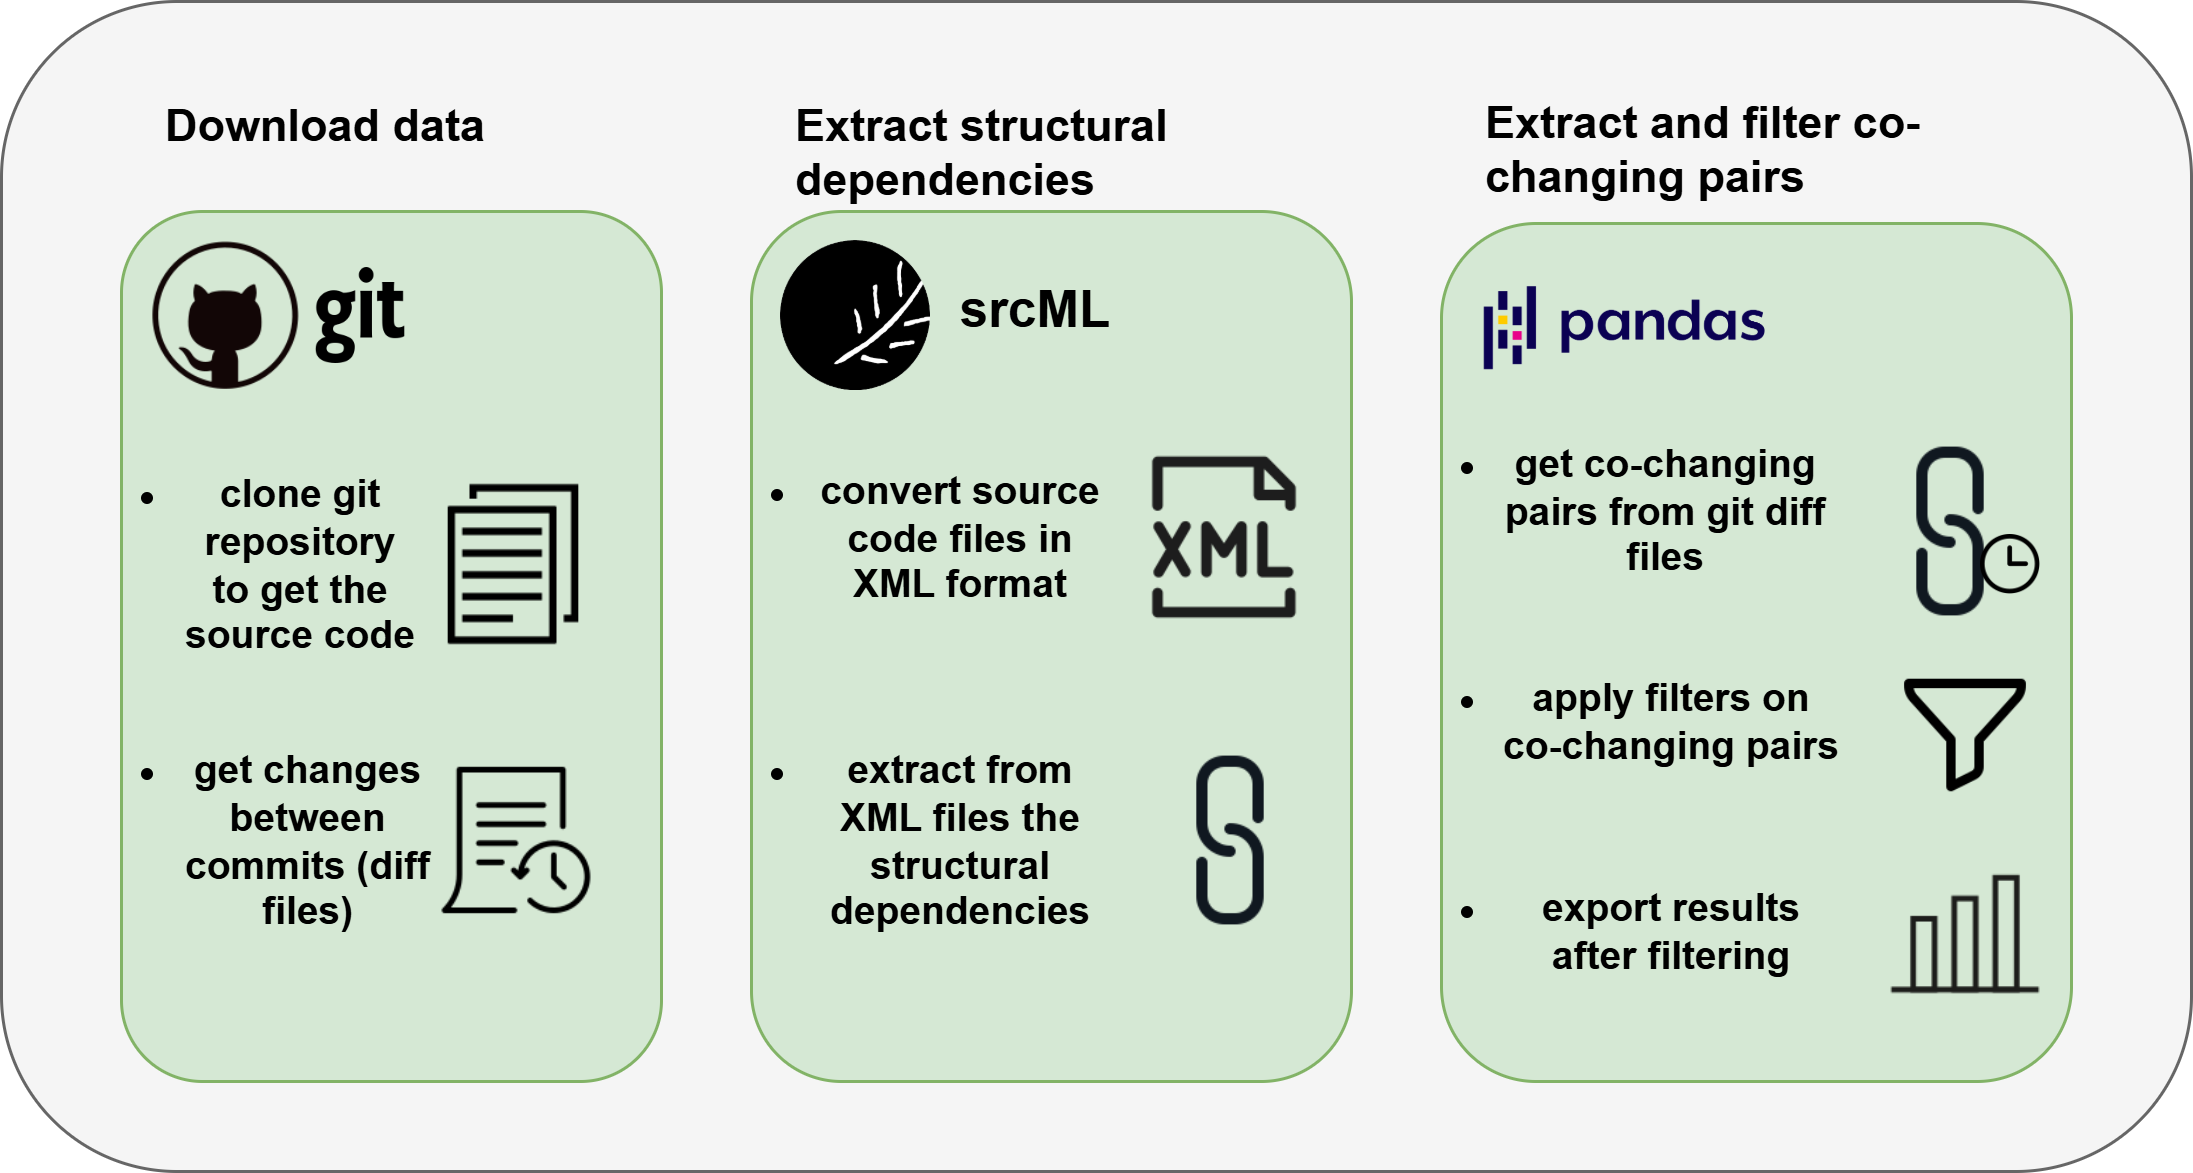
\includegraphics[width=\textwidth]{tool_workflow.png}
\caption{Tool workflow and major activities.}
\label{fig:figworkflow}
\end{figure}


\textbf{Download git data.}

The source code repository provides us all the needed information to extract both types of dependencies. It holds the code of the system but also the change history of the system. We use the source code for structural dependencies extraction and the change history for co-changing pairs extraction.
To get the source code files and the change history, we first need to know the repository URL from GitHub (GitHub is a Git repository cloud-based hosting service). With the GitHub URL and a series of Git commands, the tool can download all the necessary data for dependencies extraction.

As we can see in figure \ref{fig:figgitdata}, the \textit{"clone"} command will download a Git repository to your local computer, including the source code files. The \textit{"diff"} command will get the differences between two existing commits in the Git repository. 
The tool gets the Git repository and the source code files by executing the "clone" command. Afterward, it gets all the existing commits within the Git repository. The commits are ordered by date, beginning with the oldest one and ending with the most recent one. The tool executes the "diff" command between each commit and its parent (the previous commit). The "diff" command generates a text file that contains the differences between the two commits: code differences, the number of files changed and changed file names.


\begin{figure}[H]
\centering
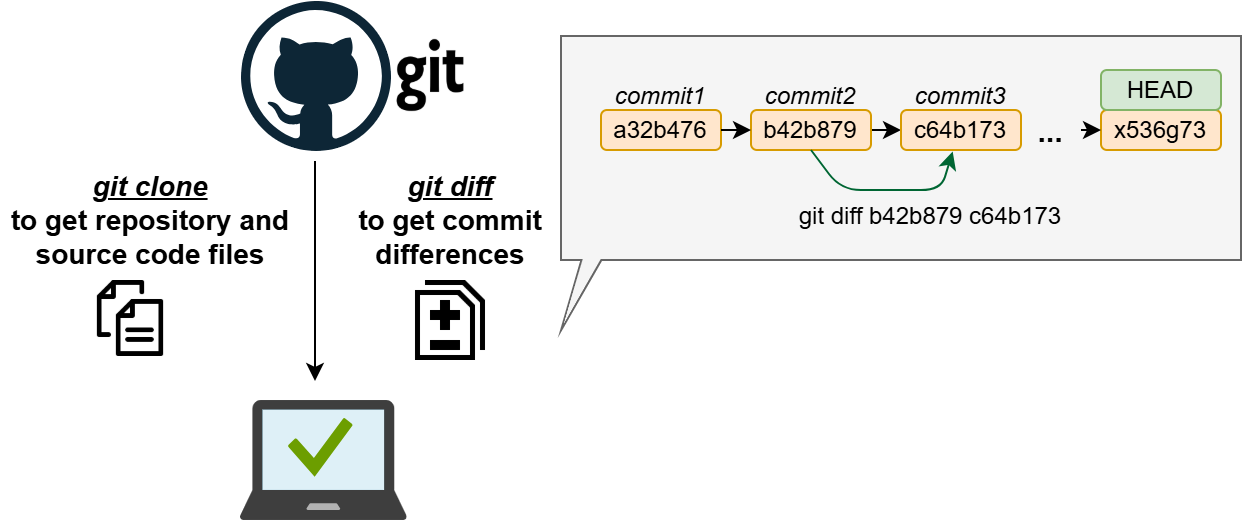
\includegraphics[width=\textwidth]{gitdata.png}
\caption{Commands used to download the required data from GitHub.}
\label{fig:figgitdata}
\end{figure}

\textbf{Extract structural dependencies.}

To extract the structural dependencies from the source code files the tool converts each source code file into srcML format using an open-source tool called srcML. The srcML format is an XML representation for source code. Each markup tag identifies elements of the abstract syntax for the language \cite{srcML}. 
After conversion, the tool parses each file and identifies all the defined entities (class, interface, enum, struct) within the file. It also identifies all the entities that are used by the entities defined.  The connection between both types of entities mentioned above constitutes a structural dependency.

\textbf{Extract and filter co-changing pairs.}

The process of extracting and filtering the co-changing pairs is represented in figure \ref{fig:figfiltering}.
For co-changing pairs extraction, the tool parses each generated diff file.
For each file, the tool gets the number of changed files and the name of the files. 
After structural dependencies extraction, the tool knows all the software entities contained in a file. Two entities from two changed files form a co-changing pair. After all the co-changing pairs of one diff file are extracted, the tool moves to the next diff file and extracts the set of co-changing pairs.

As will be presented in more details in sections \ref{sec:filtercommit}, \ref{sec:filterocc}, and \ref{sec:filterstrength}, not every co-changing pair extracted is a logical dependency. For a co-changing pair to be labeled as a logical dependency, it has to meet some criteria. Each criterion constitutes a filter that a co-changing pair has to pass in order to be called logical dependency.
The filters are implemented in the tool and can be combined. The input for each filter is the set of co-changing pairs extracted, and the output is the remaining co-changing pairs that respect the filter criterion.


\begin{figure}[H]
\centering
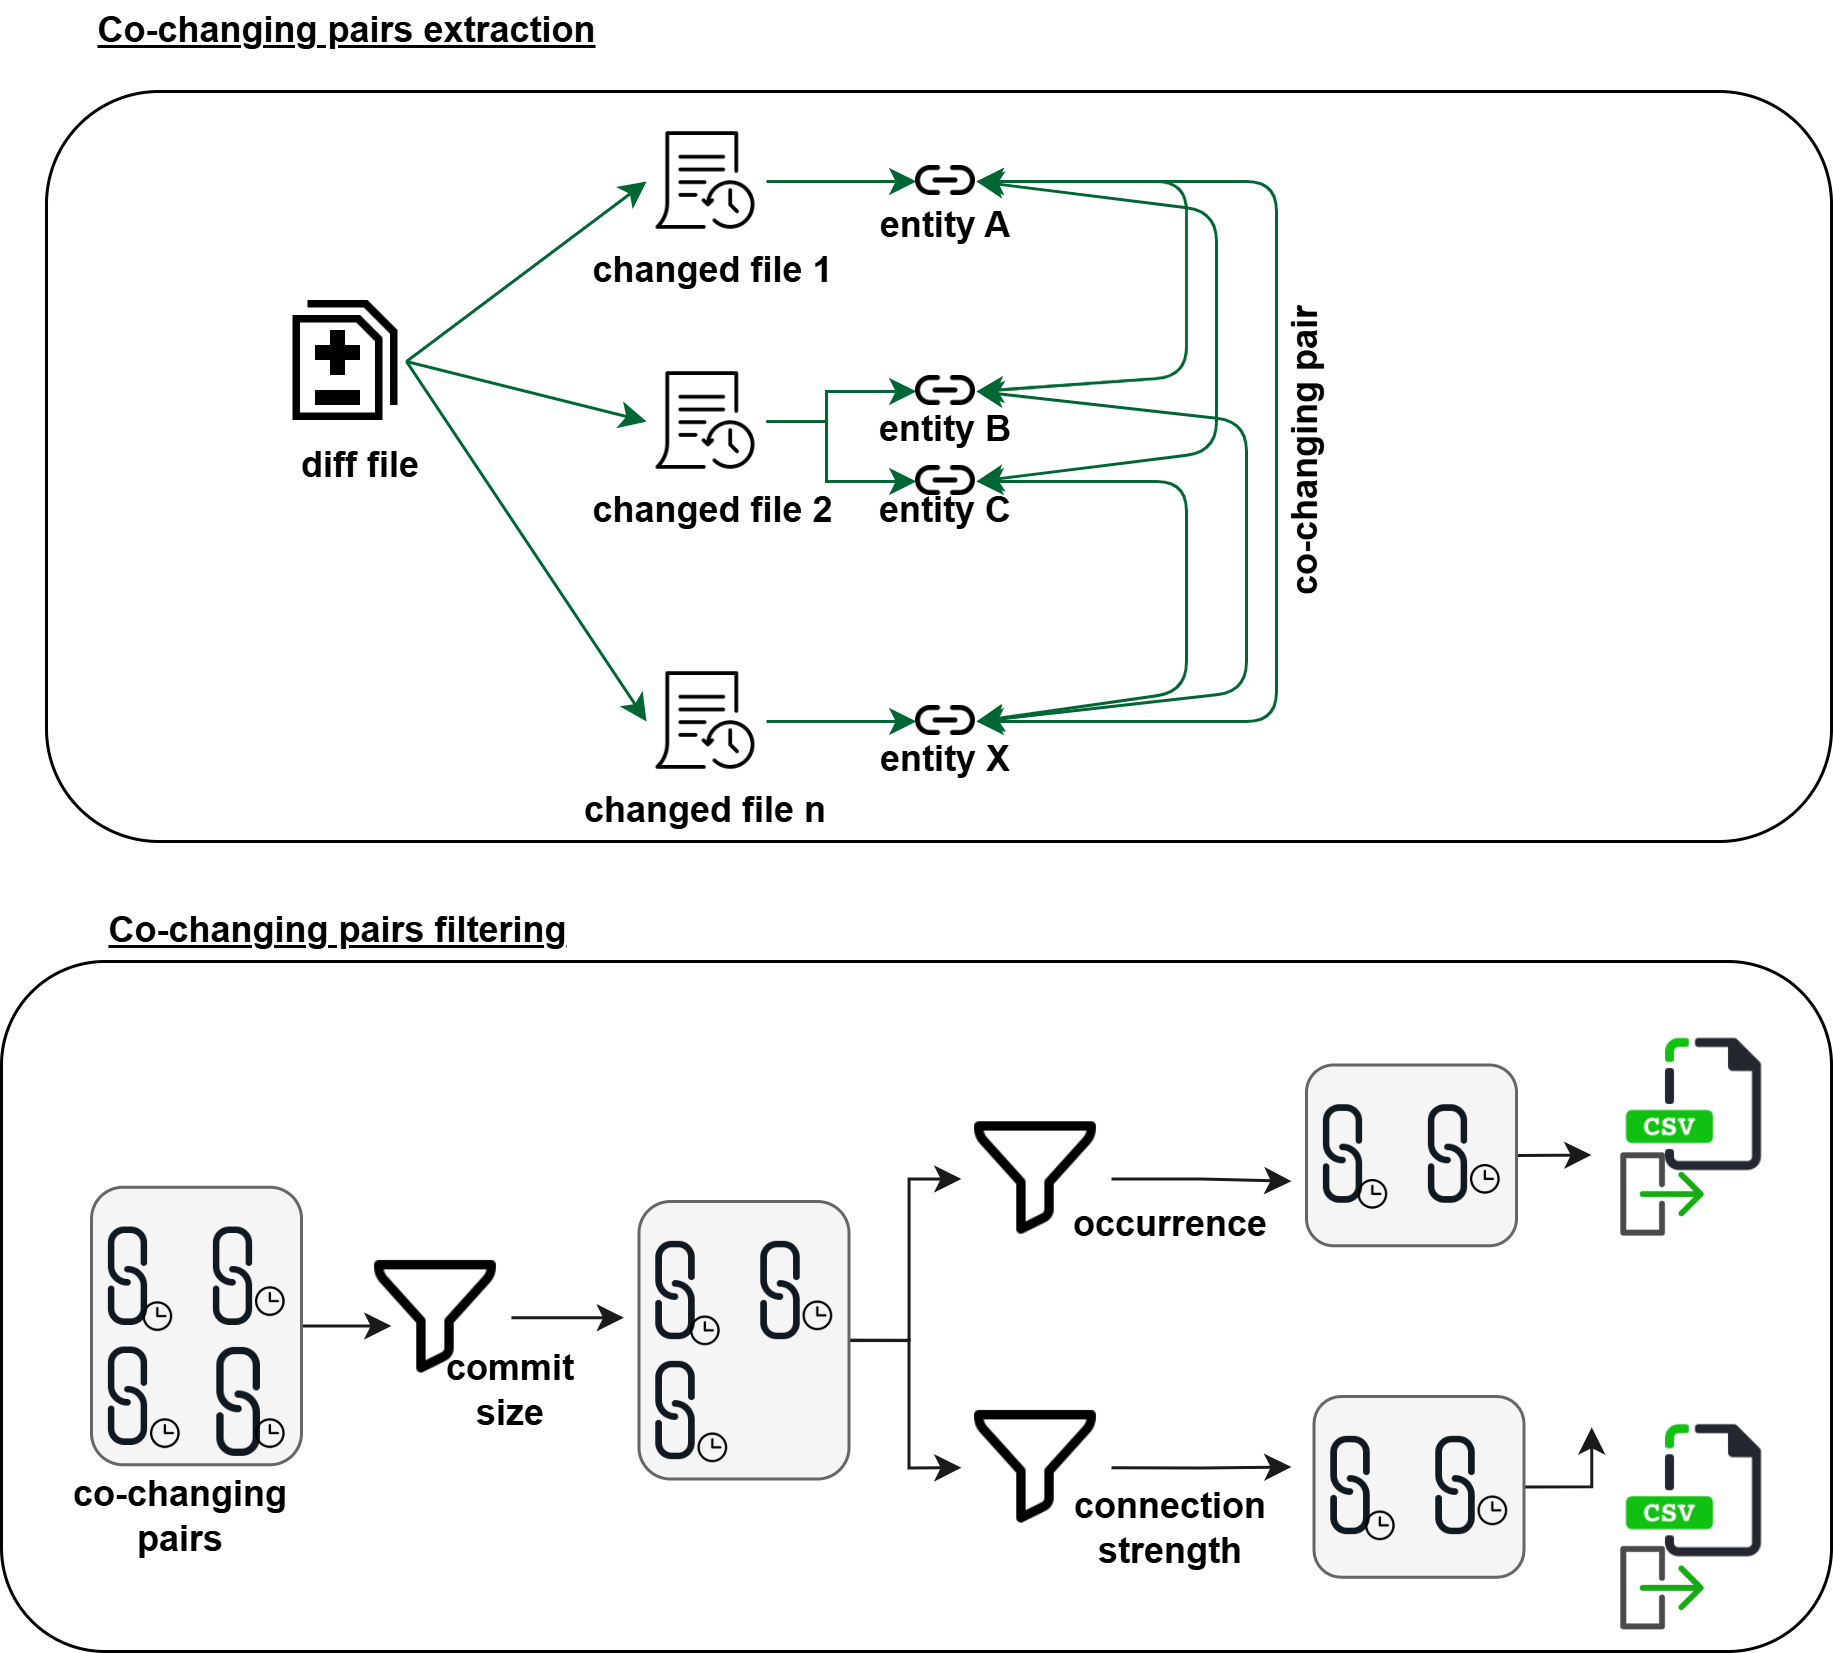
\includegraphics[width=\textwidth]{pairs_filtering.png}
\caption{Co-changing pairs extraction and filtering.}
\label{fig:figfiltering}
\end{figure}


\chapter {Filtering extracted co-changing pairs in order to obtain logical dependencies}

\section{Data set used}
\label{sec:dataset}
We have analyzed a set of open-source projects found on GitHub\footnote{http://github.com/} \cite{Kalliamvakou2016} in order to extract the structural and logical dependencies between classes. Table \ref{table:1} enumerates all the systems studied. The 1st column assigns the projects IDs; 2nd column shows the project name; 3rd column shows the number of entities(classes and interfaces) extracted; 4th column shows the number of most recent commits analyzed from the active branch of each project and the 5th shows the language in which the project was developed.


\begin{table}[!h]
\renewcommand{\arraystretch}{1}
\caption{Summary of open source projects studied.}
\label{table:1}
\centering
\scalebox{0.9}{
\begin{tabular}{|c|c|c|c|c|c|}
\hline
   ID  & Project    & Nr. of & Nr. of& Type\\
     &     & entites & commits & \\
\hline
1	&	bluecove	&	2685	&	894	&	java	\\
2	&	aima-java	&	5232	&	1006	&	java	\\
3	&	powermock	&	2801	&	949	&	java	\\
4	&	restfb	&	3350	&	1391	&	java	\\
5	&	rxjava	&	21097	&	4398	&	java	\\
6	&	metro-jax-ws	&	6482	&	2927	&	java	\\
7	&	mockito	&	5189	&	3330	&	java	\\
8	&	grizzly	&	10687	&	3113	&	java	\\
9	&	shipkit	&	639	&	1563	&	java	\\
10	&	OpenClinica	&	9655	&	3276	&	java	\\
11	&	robolectric	&	8922	&	5912	&	java	\\
12	&	aeron	&	4159	&	5977	&	java	\\
13	&	antlr4	&	4747	&	4431	&	java	\\
14	&	mcidasv	&	3272	&	4136	&	java	\\
15	&	ShareX	&	4289	&	5485	&	csharp	\\
16	&	aspnetboilerplate	&	9712	&	4323	&	csharp	\\
17	&	orleans	&	16963	&	3995	&	csharp	\\
18	&	cli	&	2063	&	4488	&	csharp	\\
19	&	cake	&	12260	&	2518	&	csharp	\\
20	&	Avalonia	&	16732	&	5264	&	csharp	\\
21	&	EntityFrameworkCore	&	50179	&	5210	&	csharp	\\
22	&	jellyfin	&	8764	&	5433	&	csharp	\\
23	&	PowerShell	&	2405	&	3250	&	csharp	\\
24	&	WeiXinMPSDK	&	7075	&	5729	&	csharp	\\
25	&	ArchiSteamFarm	&	702	&	2497	&	csharp	\\
26	&	VisualStudio	&	4869	&	5039	&	csharp	\\
27	&	CppSharp	&	17060	&	4522	&	csharp	\\

\hline
\end{tabular}
}
\end{table}



\section{Filtering based on the size of commit transactions}
\label{sec:filtercommit}

As presented in section \ref{sec:copairs_extraction}, according to surveys,  co-changing pairs are not used because of their size. One system can have millions of co-changing pairs.
With this filtering type, we not only want to decrease the total size of the extracted co-changing pairs. But also to be one step closer to the identification of the logical dependencies among the co-changing pairs.
In this step, we want to filter the co-changing pairs extracted after commit size (cs). This means that the co-changing pairs are extracted only from commits that involve fewer files than an established threshold number. 

Different works have chosen fixed threshold values for the maximum number of files accepted in a commit. Cappiluppi and Ajienka, in their works \cite{DBLP:journals/jss/AjienkaC17}, \cite{DBLP:journals/ese/AjienkaCC18} only take into consideration commits with less then 10 source code files changed in building the logical dependencies.

The research of Beck et al \cite{Beck:2011:CMC:2025113.2025162} only takes in consideration transactions with up to 25 files. The research \cite{Oliva:2011:ISL:2067853.2068086} provided also a quantitative analysis of the number of files per revision; Based on the analysis of 40,518 revisions, the mean value obtained for the number of files in a revision is 6 files. However, standard deviation value shows that the dispersion is high. 

We analyzed the overall transaction size trend for 27 open-source csharp and java systems with a total of 74 332 commits. The results are presented in Figure \ref{fig:fig_cs} and in table \ref{table:cs_values}, based on them we can say that 90\% of the total commit transactions made are with less than 10 source code files changed. This percent allows us to say that setting a threshold of 10 files for the maximum size of the commit transactions will not affect so much the total number of commit transactions from the systems since it will still remain 90\% of the commit transactions from where we can extract co-changing pairs \cite{DepSACI}.


\begin{figure}[!h]
\centering
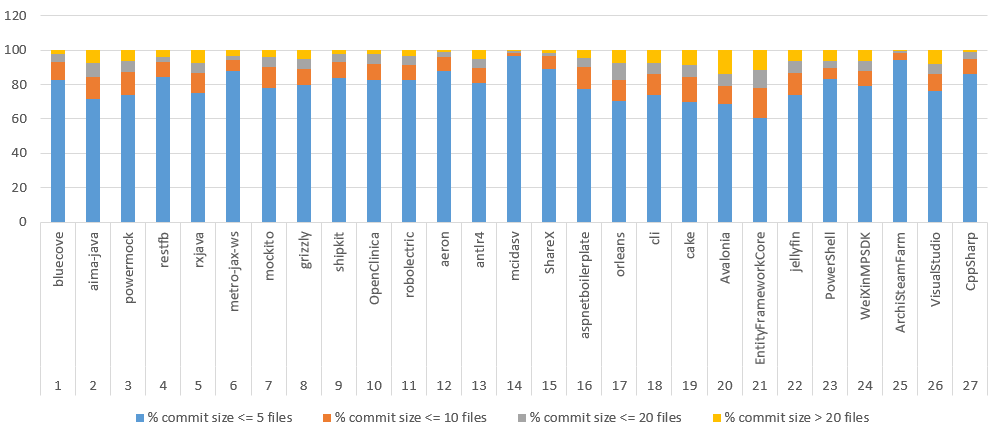
\includegraphics[width=\textwidth]{commit_distribution.png}
\caption{Commit transaction size(cs) trend in percentages.}
\label{fig:fig_cs}
\centering
\end{figure}


\begin{figure}[!h]
\centering
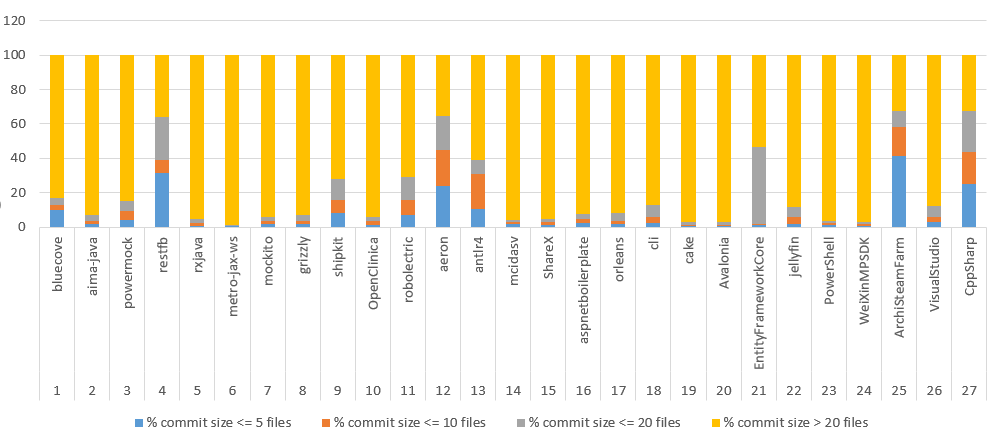
\includegraphics[width=\textwidth]{ld_distribution.png}
\caption{Percentages of LD extracted from each commit transaction size(cs) group.}
\label{fig:fig_ld_cs}
\centering
\end{figure}

As we can see in Figure \ref{fig:fig_ld_cs} even though only 5\% of the commit transactions have more than 20 files changed ($20<cs<inf$) they generate in average 80\% of the total amount of co-changing pairs extracted from the systems.
The high number of co-changing pairs extracted from such a small number of commit transactions is caused by the number of files involved in those commit transactions. 

One single commit transaction can lead to a large amount of co-changing pairs. For example in RxJava we have commit transactions with 1030 source code files, this means that those commits can generate 
$\Comb{n}{k}=\frac{n!}{k!(n-k)!} = \frac{1030!}{2!(1028)!} = 529 935$ logical dependencies. By setting a threshold on the commit transaction size we can avoid the introduction of those co-changing pairs into the system.



So filtering 10\% of the total amount of commit transactions can lead to a significant decrease of the amount of co-changing pairs and that is why we choose the value of 10 files as our fixed threshold for the maximum size of a commit transaction \cite{DepSACI}.



\begin{table}[!h]
\renewcommand{\arraystretch}{1}
\caption{Commit transaction size(cs) trend and average per system.}
\label{table:cs_values}
\centering
\scalebox{0.9}{
\begin{tabular}{|c|c|c|c|c|c|c|}
\hline
Nr.	  & Project    &	$cs\leq 5$	&	$cs\leq 10$	&	$cs\leq 20$	&	$cs<\infty$ & Avg	\\ 
\hline
1	&	bluecove	&	738	&	97	&	37	&	22	&	4.9	\\
2	&	aima-java	&	733	&	134	&	74	&	65	&	7.24	\\
3	&	powermock	&	685	&	128	&	66	&	70	&	9.61	\\
4	&	restfb	&	1160	&	127	&	44	&	60	&	9.9	\\
5	&	rxjava	&	3395	&	447	&	253	&	303	&	8.46	\\
6	&	metro-jax-ws	&	2583	&	198	&	78	&	68	&	4.33	\\
7	&	mockito	&	2522	&	433	&	222	&	153	&	6.33	\\
8	&	grizzly	&	2487	&	302	&	180	&	144	&	5.28	\\
9	&	shipkit	&	1311	&	151	&	64	&	37	&	4.26	\\
10	&	OpenClinica	&	2837	&	250	&	119	&	70	&	3.31	\\
11	&	robolectric	&	4827	&	503	&	264	&	318	&	7.43	\\
12	&	aeron	&	4844	&	684	&	300	&	149	&	4.6	\\
13	&	antlr4	&	3426	&	437	&	304	&	264	&	8.5	\\
14	&	mcidasv	&	3996	&	81	&	35	&	24	&	2.47	\\
15	&	ShareX	&	4731	&	529	&	145	&	80	&	4.69	\\
16	&	aspnetboilerplate	&	3208	&	569	&	321	&	225	&	6.61	\\
17	&	orleans	&	2780	&	518	&	369	&	328	&	8.95	\\
18	&	cli	&	3377	&	551	&	308	&	252	&	6.43	\\
19	&	cake	&	1785	&	359	&	174	&	200	&	9.89	\\
20	&	Avalonia	&	3806	&	641	&	371	&	446	&	8.43	\\
21	&	EntityFrameworkCore	&	2866	&	878	&	644	&	822	&	15.38	\\
22	&	jellyfin	&	4007	&	662	&	419	&	345	&	6.25	\\
23	&	PowerShell	&	2702	&	224	&	133	&	191	&	7.33	\\
24	&	WeiXinMPSDK	&	4604	&	526	&	296	&	303	&	9.01	\\
25	&	ArchiSteamFarm	&	2357	&	92	&	28	&	20	&	2.24	\\
26	&	VisualStudio	&	3902	&	521	&	295	&	321	&	6.71	\\
27	&	CppSharp	&	3870	&	390	&	203	&	59	&	3.28	\\
\hline
\end{tabular}
}
\end{table}





\section{Filtering based on number of occurrences}
\label{sec:filterocc}

In the previous section, we filtered the co-changing pairs based on the commit size. Even though the number of extracted co-changing pairs was reduced, this type of filtering will not guarantee that the remaining co-changing pairs can pass as logical dependencies. 
One occurrence of a co-change pair can be a valid logical dependency, but can also be a coincidence. 

Taking into consideration only co-changing pairs with multiple occurrences as valid dependencies can lead to more accurate results. But, if the project studied has a relatively small amount of commits, the probability to find multiple updates of the same classes at the same time is less likely to happen, so filtering after the number of occurrences can lead to filtering all the co-changes extracted.

We have performed a series of analyses on the test systems, incrementing the threshold value occurrence (occ) from 1 to 4. The co-changing pairs are extracted only for commits with the commit transaction size less or equal to 10. For each threshold mentioned above, the extracted co-changing pairs are filtered again by the occurrence threshold established. All the co-changing pairs that do not exceed the minimum number of occurrences are discarded.

The results of the analysis are presented in Table \ref{table:sd_percentages} as percentages of co-changing pairs that are also structural dependencies and Table \ref{table:ld_ratio} as ratio of the number of co-changing pairs to the number of structural dependencies (SD).


\begin{table}[!h]
\renewcommand{\arraystretch}{1}
\caption{Percentage of co-changing pairs that are also structural dependencies.}
\label{table:sd_percentages}
\centering
\scalebox{0.9}{
\begin{tabular}{|c|c|c|c|c|}
\hline
    ID  & $occ\geq 1$ & $occ\geq 2$ & $occ\geq 3$ & $occ\geq 4$  \\
\hline
1	&	7,13	&	7,77	&	7,99	&	19,71	\\
2	&	19,54	&	25,76	&	29,55	&	32,16	\\
3	&	6,66	&	8,58	&	11,82	&	14,87	\\
4	&	1,16	&	1,17	&	0,91	&	0,80	\\
5	&	3,99	&	3,96	&	7,75	&	7,49	\\
6	&	13,92	&	20,16	&	22,91	&	22,77	\\
7	&	8,38	&	9,28	&	14,93	&	14,58	\\
8	&	6,70	&	9,73	&	14,20	&	15,60	\\
9	&	16,98	&	23,34	&	29,22	&	32,89	\\
10	&	8,94	&	9,15	&	11,05	&	10,59	\\
11	&	4,99	&	6,92	&	8,88	&	11,08	\\
12	&	13,19	&	17,15	&	18,60	&	19,57	\\
13	&	2,43	&	5,59	&	8,33	&	8,21	\\
14	&	13,27	&	18,88	&	19,02	&	19,28	\\
15	&	12,90	&	21,95	&	25,51	&	27,01	\\
16	&	13,33	&	17,34	&	18,53	&	16,24	\\
17	&	6,09	&	6,18	&	6,41	&	6,44	\\
18	&	9,73	&	10,60	&	14,27	&	18,80	\\
19	&	10,26	&	13,54	&	13,64	&	12,60	\\
20	&	12,83	&	18,36	&	21,00	&	25,72	\\
21	&	2,86	&	4,65	&	5,70	&	4,98	\\
22	&	5,20	&	6,56	&	8,18	&	8,90	\\
23	&	8,23	&	13,64	&	17,04	&	17,65	\\
24	&	6,77	&	10,89	&	14,47	&	16,05	\\
25	&	9,85	&	10,15	&	11,65	&	11,33	\\
26	&	8,65	&	10,79	&	12,78	&	14,34	\\
27	&	7,04	&	8,78	&	9,87	&	10,08	\\
\hline
Avg	&	8,93	&	11,88	&	14,23	&	15,55	\\
\hline
\end{tabular}
}
\end{table}


\begin{table}[!h]
\renewcommand{\arraystretch}{1}
\caption{Ratio of number of co-changing pairs to number of structural dependencies. }
\label{table:ld_ratio}
\centering
\scalebox{0.9}{
\begin{tabular}{|c|c|c|c|c|}
\hline
    ID  & $occ\geq 1$ & $occ\geq 2$ & $occ\geq 3$ & $occ\geq 4$  \\
\hline
1	&	4,13	&	1,94	&	1,23	&	0,26	\\
2	&	0,81	&	0,33	&	0,16	&	0,10	\\
3	&	5,12	&	1,93	&	0,78	&	0,38	\\
4	&	53,36	&	42,00	&	38,31	&	36,30	\\
5	&	4,27	&	2,90	&	0,88	&	0,72	\\
6	&	1,07	&	0,46	&	0,30	&	0,23	\\
7	&	4,09	&	2,38	&	0,99	&	0,73	\\
8	&	4,06	&	1,57	&	0,76	&	0,49	\\
9	&	3,64	&	2,03	&	1,14	&	0,77	\\
10	&	1,41	&	1,01	&	0,47	&	0,34	\\
11	&	7,91	&	4,47	&	2,93	&	2,03	\\
12	&	3,92	&	2,15	&	1,47	&	1,07	\\
13	&	10,15	&	3,18	&	1,22	&	1,03	\\
14	&	3,07	&	1,53	&	1,16	&	0,97	\\
15	&	2,34	&	0,84	&	0,48	&	0,33	\\
16	&	1,21	&	0,47	&	0,26	&	0,19	\\
17	&	2,99	&	1,83	&	1,11	&	0,84	\\
18	&	2,26	&	1,37	&	0,67	&	0,40	\\
19	&	2,32	&	1,38	&	0,76	&	0,67	\\
20	&	1,24	&	0,58	&	0,35	&	0,18	\\
21	&	5,33	&	2,12	&	1,27	&	1,05	\\
22	&	3,38	&	1,88	&	0,99	&	0,74	\\
23	&	3,62	&	1,22	&	0,76	&	0,37	\\
24	&	2,57	&	1,22	&	0,67	&	0,46	\\
25	&	7,47	&	5,36	&	4,16	&	3,73	\\
26	&	4,03	&	2,16	&	1,50	&	1,15	\\
27	&	7,46	&	4,26	&	2,99	&	2,43	\\
\hline
Avg	&	5,67	&	3,43	&	2,51	&	2,15	\\
\hline
\end{tabular}
}
\end{table}

Based on Table \ref{table:sd_percentages} we can say that only a small percentage of the extracted co-changing pairs are also structural dependencies. This is consistent with the findings of related works \cite{DBLP:journals/jss/AjienkaC17}, \cite{DBLP:journals/ese/AjienkaCC18}. 
The percentage of co-changing pairs that are also structural dependencies increases with the minimum number of occurrences because the number of co-changing pairs from the systems decreases with the minimum number of occurrences. 
We calculate the overlapping between co-changing pairs and structural dependencies not only because we want to get an idea of how many structural dependencies are reflected in the versioning system through co-changing pairs, but also because we want to eliminate co-changing pairs that are structural dependencies since they don't bring any new information about the system.

We stopped the minimum occurrences threshold to 4 because we observed that for systems with ID 2, 6, 10, and 16 from Table \ref{table:ld_ratio} the ratio number is lower than 1, which means that the number of structural dependencies is higher than the number of co-changing pairs. On the other hand, for systems with ID 4, 11, 25, 27, the threshold of 4 for a minimum number of occurrences does not change the discrepancy between the number of co-changing pairs and structural dependencies.

If we try to go higher with the occurrences threshold, we will risk filtering all the existing co-changing pairs for some systems.
So, filtering with a threshold of 4 for the minimum number of occurrences will indeed filter the logical dependencies, but for some of the systems, the remaining number of co-changing pairs will still be significantly higher compared to the number of structural dependencies.




\section{Filtering based on connection strength}
\label{sec:filterstrength}

In section \ref{sec:filtercommit} we filtered the co-changing pairs extracted from the versioning system history based on the commit size. Based on the results obtained, we decided to filter out all co-changing pairs extracted from commits with more than 10 files changed. 

In section \ref{sec:filterocc}, we added a new filtering rule based on the occurrence of a co-changing pair. The new filter is applied to the co-changing pairs resulted after commit size filtering. In this case, the filtering method proved insufficient due to the size diversity of the systems. One important conclusion drawn from the occurrence number filtering is that setting a hard threshold for a filter is not always a good idea. One threshold value can be too much for a small-sized system and too little for a medium-sized system. 

To avoid the above problem, we decided to introduce another filter complementary to the commit size filter described in section \ref{sec:filtercommit}.
This filter focuses on the connection strength of a co-changing pair. In this section, we will filter out all the co-changing pairs that are not strongly connected.

To determine the connection strength of a pair, we first need to calculate the connection factors for both entities that form a co-changing pair.
Assuming that we have a co-changing pair formed by entities A and B, the connection factor of entity A with entity B is the percentage from the total commits involving A that contains entity B. The connection factor of entity B with entity A is the percentage from the total commits involving B that contain also entity A.

\begin{equation}
 connection\ factor\ for\ A = \frac{100 * commits\ involving\ A\ and\ B}{total\ nr\ of\ commits\ involving\ A}
\end{equation}

\begin{equation}
 connection\ factor\ for\ B = \frac{100 * commits\ involving\ A\ and\ B}{total\ nr\ of\ commits\ involving\ B}
\end{equation}

As a practical example, if the pair formed by A and B update together 7 times and the total number of commits involving A is 20 and involving B is 7. The factor for A is 35 and for B is 100. The factor of 100 is the maximum factor that you can have and means that in all the commits involving B, also A is present.

Due to the fact that the factors obtained can vary from 0 to 100, for this filter, we begin with a threshold value of 10 and increment it by 10 until we reach 100. 

The co-changing pairs are filtered out based on two scenarios:
\begin{itemize}
	\item factor A and factor B $\geq threshold \%$ 
	\item factor A or factor B $\geq threshold \%$ 
\end{itemize}

\begin{table}[!h]
\renewcommand{\arraystretch}{1}
\caption{Ratio of number of filtered co-changing pairs to number of SD, when factor A and factor B $\geq threshold \%$ }
\label{tab:commitstrengthAND}
\centering
\scalebox{0.8}{
\begin{tabular}{|c|cccccccccc|c|}
\hline
Project &	$\geq10\%$	&	$\geq20\%$		&	$\geq30\%$		&	$\geq40\%$		&	$\geq50\%$		&	$\geq60\%$		&	$\geq70\%$		&	$\geq80\%$		&	$\geq90\%$		&	$\geq100\%$	 \\
\hline
bluecove	&	1.326	&	0.658	&	0.433	&	0.401	&	0.244	&	0.199	&	0.195	&	0.022	&	0.011	&	0.011	\\
aima-java	&	0.266	&	0.137	&	0.070	&	0.044	&	0.036	&	0.019	&	0.005	&	0.004	&	0.003	&	0.003	\\
powermock	&	0.505	&	0.243	&	0.147	&	0.086	&	0.061	&	0.031	&	0.031	&	0.031	&	0.031	&	0.031	\\
restfb	&	0.822	&	0.163	&	0.045	&	0.017	&	0.011	&	0.002	&	0.001	&	0.001	&	0.001	&	0.001	\\
rxjava	&	0.234	&	0.119	&	0.054	&	0.037	&	0.034	&	0.018	&	0.013	&	0.011	&	0.007	&	0.007	\\
metro-jax-ws	&	0.227	&	0.155	&	0.101	&	0.077	&	0.070	&	0.036	&	0.018	&	0.017	&	0.016	&	0.016	\\
mockito	&	1.590	&	0.804	&	0.357	&	0.288	&	0.215	&	0.088	&	0.052	&	0.036	&	0.032	&	0.032	\\
grizzly	&	2.073	&	0.293	&	0.170	&	0.111	&	0.093	&	0.050	&	0.039	&	0.034	&	0.021	&	0.007	\\
shipkit	&	1.495	&	0.479	&	0.271	&	0.142	&	0.108	&	0.059	&	0.047	&	0.011	&	0.008	&	0.008	\\
OpenClinica	&	0.253	&	0.135	&	0.093	&	0.078	&	0.062	&	0.042	&	0.024	&	0.019	&	0.019	&	0.017	\\
robolectric	&	0.114	&	0.086	&	0.064	&	0.037	&	0.027	&	0.025	&	0.001	&	0.000	&	0.000	&	0.000	\\
aeron	&	0.277	&	0.136	&	0.085	&	0.069	&	0.053	&	0.045	&	0.039	&	0.015	&	0.007	&	0.004	\\
antlr4	&	11.363	&	0.721	&	0.031	&	0.010	&	0.007	&	0.004	&	0.000	&	0.000	&	0.000	&	0.000	\\
mcidasv	&	3.225	&	0.805	&	0.660	&	0.533	&	0.493	&	0.454	&	0.386	&	0.356	&	0.005	&	0.005	\\
ShareX	&	6.097	&	0.725	&	0.663	&	0.564	&	0.500	&	0.242	&	0.176	&	0.170	&	0.001	&	0.001	\\
aspnetboilerplate	&	1.302	&	0.333	&	0.219	&	0.146	&	0.094	&	0.045	&	0.014	&	0.008	&	0.007	&	0.007	\\
orleans	&	0.816	&	0.640	&	0.551	&	0.503	&	0.496	&	0.196	&	0.159	&	0.152	&	0.142	&	0.142	\\
cli	&	1.676	&	0.233	&	0.159	&	0.118	&	0.102	&	0.062	&	0.058	&	0.029	&	0.026	&	0.026	\\
cake	&	2.335	&	0.753	&	0.614	&	0.337	&	0.075	&	0.021	&	0.007	&	0.004	&	0.004	&	0.004	\\
Avalonia	&	0.846	&	0.117	&	0.098	&	0.018	&	0.013	&	0.002	&	0.001	&	0.001	&	0.001	&	0.001	\\
EntityFrameworkCore	&	3.377	&	1.691	&	1.608	&	1.584	&	1.576	&	1.310	&	0.001	&	0.001	&	0.001	&	0.001	\\
jellyfin	&	0.132	&	0.006	&	0.003	&	0.002	&	0.002	&	0.000	&	0.000	&	0.000	&	0.000	&	0.000	\\
PowerShell	&	1.732	&	1.299	&	0.158	&	0.053	&	0.007	&	0.001	&	0.000	&	0.000	&	0.000	&	0.000	\\
WeiXinMPSDK	&	3.295	&	0.334	&	0.188	&	0.061	&	0.017	&	0.006	&	0.003	&	0.001	&	0.000	&	0.000	\\
ArchiSteamFarm	&	0.897	&	0.479	&	0.429	&	0.423	&	0.412	&	0.403	&	0.339	&	0.009	&	0.001	&	0.000	\\
VisualStudio	&	1.281	&	0.090	&	0.053	&	0.028	&	0.020	&	0.013	&	0.006	&	0.001	&	0.001	&	0.001	\\
CppSharp	&	99.528	&	1.020	&	0.992	&	0.980	&	0.972	&	0.927	&	0.078	&	0.075	&	0.073	&	0.072	\\

\hline
\end{tabular}
}
\end{table}


\begin{table}[!h]
\renewcommand{\arraystretch}{1}
\caption{Ratio of number of filtered co-changing pairs to number of SD,
 when factor A or factor B $\geq threshold \%$ }
\label{tab:commitstrengthOR}
\centering
\scalebox{0.8}{
\begin{tabular}{|c|cccccccccc|c|}
\hline
Project &	$\geq10\%$	&	$\geq20\%$		&	$\geq30\%$		&	$\geq40\%$		&	$\geq50\%$		&	$\geq60\%$		&	$\geq70\%$		&	$\geq80\%$		&	$\geq90\%$		&	$\geq100\%$	 \\
\hline
bluecove	&	1.312	&	1.181	&	0.700	&	0.599	&	0.419	&	0.235	&	0.219	&	0.046	&	0.045	&	0.045	\\
aima-java	&	0.430	&	0.280	&	0.176	&	0.118	&	0.103	&	0.056	&	0.022	&	0.020	&	0.020	&	0.020	\\
powermock	&	0.508	&	0.328	&	0.234	&	0.179	&	0.150	&	0.092	&	0.091	&	0.091	&	0.091	&	0.091	\\
restfb	&	0.662	&	0.336	&	0.122	&	0.067	&	0.059	&	0.016	&	0.015	&	0.015	&	0.015	&	0.015	\\
rxjava	&	0.279	&	0.206	&	0.145	&	0.100	&	0.099	&	0.047	&	0.044	&	0.039	&	0.034	&	0.034	\\
metro-jax-ws	&	0.271	&	0.261	&	0.204	&	0.172	&	0.160	&	0.106	&	0.082	&	0.081	&	0.080	&	0.080	\\
mockito	&	2.481	&	1.521	&	0.904	&	0.623	&	0.411	&	0.199	&	0.128	&	0.107	&	0.101	&	0.101	\\
grizzly	&	1.332	&	0.838	&	0.515	&	0.320	&	0.288	&	0.142	&	0.117	&	0.106	&	0.090	&	0.076	\\
shipkit	&	1.376	&	1.083	&	0.725	&	0.515	&	0.424	&	0.191	&	0.149	&	0.105	&	0.094	&	0.094	\\
OpenClinica	&	0.830	&	0.434	&	0.314	&	0.256	&	0.217	&	0.130	&	0.093	&	0.082	&	0.080	&	0.072	\\
robolectric	&	0.366	&	0.122	&	0.088	&	0.046	&	0.031	&	0.027	&	0.003	&	0.002	&	0.002	&	0.002	\\
aeron	&	0.781	&	0.449	&	0.265	&	0.190	&	0.160	&	0.096	&	0.062	&	0.031	&	0.021	&	0.018	\\
antlr4	&	11.363	&	0.798	&	0.055	&	0.022	&	0.011	&	0.007	&	0.002	&	0.002	&	0.002	&	0.002	\\
mcidasv	&	1.932	&	1.203	&	0.858	&	0.682	&	0.579	&	0.473	&	0.396	&	0.365	&	0.013	&	0.013	\\
ShareX	&	2.681	&	1.292	&	0.916	&	0.730	&	0.593	&	0.287	&	0.210	&	0.201	&	0.017	&	0.017	\\
aspnetboilerplate	&	1.055	&	0.759	&	0.493	&	0.364	&	0.273	&	0.130	&	0.067	&	0.050	&	0.046	&	0.046	\\
orleans	&	1.120	&	0.962	&	0.849	&	0.750	&	0.744	&	0.559	&	0.482	&	0.476	&	0.466	&	0.466	\\
cli	&	1.676	&	0.762	&	0.560	&	0.434	&	0.375	&	0.269	&	0.237	&	0.149	&	0.142	&	0.142	\\
cake	&	1.883	&	1.197	&	1.001	&	0.541	&	0.185	&	0.103	&	0.019	&	0.013	&	0.013	&	0.013	\\
Avalonia	&	0.510	&	0.224	&	0.138	&	0.037	&	0.028	&	0.011	&	0.006	&	0.003	&	0.003	&	0.003	\\
EntityFrameworkCore	&	2.636	&	1.888	&	1.695	&	1.623	&	1.608	&	1.317	&	0.006	&	0.006	&	0.006	&	0.006	\\
jellyfin	&	0.132	&	0.030	&	0.016	&	0.011	&	0.008	&	0.003	&	0.002	&	0.002	&	0.002	&	0.002	\\
PowerShell	&	3.454	&	1.648	&	0.232	&	0.081	&	0.021	&	0.004	&	0.003	&	0.003	&	0.003	&	0.003	\\
WeiXinMPSDK	&	1.342	&	0.603	&	0.327	&	0.144	&	0.080	&	0.047	&	0.015	&	0.008	&	0.007	&	0.007	\\
ArchiSteamFarm	&	5.472	&	1.416	&	0.830	&	0.677	&	0.575	&	0.450	&	0.353	&	0.023	&	0.016	&	0.014	\\
VisualStudio	&	1.281	&	0.236	&	0.142	&	0.092	&	0.060	&	0.040	&	0.031	&	0.020	&	0.019	&	0.019	\\
CppSharp	&	55.038	&	1.343	&	1.106	&	1.044	&	1.030	&	0.983	&	0.449	&	0.443	&	0.441	&	0.439	\\


\hline
\end{tabular}
}
\end{table}


In table \ref{tab:commitstrengthAND} we have on the columns the ratio between the number of structural dependencies and the number of co-changing pairs that resulted after filtering out pairs that have at least one factor below the specified threshold in the column header.
In table \ref{tab:commitstrengthOR} we have on the columns the ratio between the number of structural dependencies and the number of co-changing pairs that resulted after filtering out pairs that have both factors below the specified threshold in the column header.

We calculate the ratio number between the co-changing pairs and the structural dependencies because we want to evaluate the size of the extracted co-changing pairs compared to the size of the structural dependencies from the system. 
According to surveys \cite{Shtern:2012:CMS:2332427.2332428}, \cite{sar}, the main reason why logical dependencies (a.k.a filtered co-changes) are not used together with structural dependencies is because of their size. So, it is important to us to get at each filtering step an overview regarding the ratio between co-changes size and structural dependencies size.

From the results presented in tables \ref{tab:commitstrengthAND} and \ref{tab:commitstrengthOR} we conclude that the number of co-changing pairs is drastically reduced. In most cases, the number of structural dependencies surpasses the number of co-changing pairs that remain after filtering. But, we do the filtering not only to reduce the size of the co-changing pairs extracted. We do the filtering of co-changing pairs extracted to make sure that the remaining co-changing pairs are indeed logically dependent.

If we filter out all the co-changing pairs that do not update at least half of the time together (factor A and factor B $\geq 50 \%$ ) we remain with a decent quantity of co-changing pairs. Given the size of the output and the connection strength of the co-changing pairs, the remaining co-changing pairs can be considered, at this point, to be logically dependent. 




\section{Overlaps between structural and co-changing pairs}
\label{sec:overlaps}

A logical dependency can be also a structural dependency and vice-versa, so studying the overlapping between logical and structural dependencies while filtering is important since the intention is to introduce those logical dependencies among with structural dependencies in architectural reconstruction systems. Current studies have shown a relatively small percentage of overlapping between them with and without any kind of filtering \cite{DBLP:journals/jss/AjienkaC17}. This means that a lot of non related entities update together in the versioning system, the goal here is to establish the factors that determine such a small percentage of overlapping \cite{enase19}.

Since we are first extracting co-changing pairs and only after various filters we call the remaining co-changing pairs logically dependent, we will be studying the overlapping between the remaining co-changing pairs after each filtering stage and the structural dependencies. 
For each system, we extracted the structural dependencies and the co-changing pairs and determined the overlap between the two dependencies sets, in various experimental conditions. 

One variable experimental condition is whether changes located in comments contribute towards logical dependencies. This condition distinguishes between two different cases: 
\begin{itemize}
	\item with comments: a change in source code files is counted as a co-changing pair, even if the change is inside comments in all files
	\item without comments: commits that changed source code files only by editing comments are ignored
\end{itemize}

In all cases, we varied the following threshold values: 
 \begin{itemize}
	\item commit size ($cs$): the maximum size of commit transactions which are accepted to generate co-changes. The values for this threshold were 5, 10, 20 and no threshold (infinity).  
	\item number of occurrences ($occ$): the minimum number of repeated occurrences for a co-change to be counted as logical dependency. The values for this threshold were 1, 2, 3 and 4.  
\end{itemize}

The six tables below present the synthesis of our experiments. 
We have computed the following  values:
\begin{itemize}
	\item the mean ratio of the number of co-changes to the number of structural dependencies (SD)
   	\item the mean percentage of structural dependencies that are also co-changes (calculated from the number of overlaps divided to the number of structural dependencies)	
	\item the mean percentage of co-changes that are also structural dependencies (calculated from the number of overlaps divided to the number of co-changes)
\end{itemize}

In all the six tables, \ref{tab:ratio:comm}, \ref{tab:ratio:nocomm}, \ref{tab:percSD:comm}, \ref{tab:percSD:nocomm},
\ref{tab:percLD:comm}, \ref{tab:percLD:nocomm} we have on columns the values used for the commit size $cs$, while on rows we have the values for the number of occurrences threshold $occ$. The tables contain median values obtained for experiments done under all combinations of the two threshold values, on all test systems. In all tables, the upper right corner corresponds to the most relaxed filtering conditions, while the lower left corner corresponds to the most restrictive filtering conditions.

\begin{table}[!h]
%% increase table row spacing, adjust to taste
\renewcommand{\arraystretch}{1}
\caption{Ratio of number of co-changes to number of SD, case with comments}
\label{tab:ratio:comm}
\centering

\begin{tabular}{|c|c|c|c|c|}
\hline
	      &	$cs\leq 5$	&	$cs\leq 10$	&	$cs\leq 20$	&	$cs<\infty$	\\
\hline
$occ\geq 1$	&	3,39	&	5,67	&	9,00	&	80,31	\\
$occ\geq 2$	&	2,24	&	3,47	&	5,02	&	60,14	\\
$occ\geq 3$	&	1,04	&	2,53	&	3,52	&	44,68	\\
$occ\geq 4$	&	0,90	&	2,16	&	2,88	&	33,47	\\
\hline
\end{tabular}
\end{table}

\begin{table}[!h]
%% increase table row spacing, adjust to taste
\renewcommand{\arraystretch}{1}
\caption{Ratio of number of co-changes to number of SD, case without comments}
\label{tab:ratio:nocomm}
\centering

\begin{tabular}{|c|c|c|c|c|}
\hline
	      &	$cs\leq 5$	&	$cs\leq 10$	&	$cs\leq 20$	&	$cs< \infty$	\\
\hline
$occ\geq 1$	&	3,24	&	5,33	&	7,90	&	67,16	\\
$occ\geq 2$	&	1,35	&	3,27	&	4,72	&	47,39	\\
$occ\geq 3$	&	1,00	&	1,67	&	2,49	&	32,39	\\
$occ\geq 4$	&	0,43	&	1,26	&	1,93	&	22,15	\\
\hline
\end{tabular}
\end{table}

\begin{table}[!h]
%% increase table row spacing, adjust to taste
\renewcommand{\arraystretch}{1}
\caption{Percentage of SD that are also co-changes, case with comments}
\label{tab:percSD:comm}
\centering

\begin{tabular}{|c|c|c|c|c|}
\hline
	      &	$cs\leq 5$	&	$cs\leq 10$	&	$cs\leq 20$	&	$cs< \infty$	\\
\hline
$occ\geq 1$	&	19,75	&	29,86	&	39,29	&	76,59	\\
$occ\geq 2$	&	12,50	&	20,20	&	27,68	&	66,11	\\
$occ\geq 3$	&	8,49	&	14,22	&	19,94	&	55,99	\\
$occ\geq 4$	&	6,58	&	10,95	&	15,76	&	47,12	\\
\hline
\end{tabular}
\end{table}

\begin{table}[!h]
%% increase table row spacing, adjust to taste
\renewcommand{\arraystretch}{1}
\caption{Percentage of SD that are also co-changes, case without comments}
\label{tab:percSD:nocomm}
\centering

\begin{tabular}{|c|c|c|c|c|}
\hline
	      &	$cs\leq 5$	&	$cs\leq 10$	&	$cs\leq 20$	&	$cs< \infty$	\\
\hline
$occ\geq 1$	&	18,88	&	28,47	&	37,44	&	71,12	\\
$occ\geq 2$	&	11,87	&	19,03	&	25,93	&	59,58	\\
$occ\geq 3$	&	8,00	&	13,09	&	18,15	&	48,65	\\
$occ\geq 4$	&	5,85	&	9,94	&	14,27	&	39,07	\\
\hline
\end{tabular}
\end{table}

\begin{table}[!h]
%% increase table row spacing, adjust to taste
\renewcommand{\arraystretch}{1}
\caption{Percentage of co-changes that are also SD, case with comments}
\label{tab:percLD:comm}
\centering

\begin{tabular}{|c|c|c|c|c|}
\hline
	      &	$cs\leq 5$	&	$cs\leq 10$	&	$cs\leq 20$	&	$cs< \infty$	\\
\hline
$occ\geq 1$	&	12,02	&	8,86	&	6,72	&	1,79	\\
$occ\geq 2$	&	15,05	&	11,71	&	9,38	&	2,21	\\
$occ\geq 3$	&	17,45	&	13,97	&	11,57	&	2,86	\\
$occ\geq 4$	&	18,96	&	15,28	&	12,94	&	3,67	\\
\hline
\end{tabular}
\end{table}

\begin{table}[!h]
%% increase table row spacing, adjust to taste
\renewcommand{\arraystretch}{1}
\caption{Percentage of co-changes that are also SD, case without comments}
\label{tab:percLD:nocomm}
\centering
\begin{tabular}{|c|c|c|c|c|}
\hline
	      &	$cs\leq 5$	&	$cs\leq 10$	&	$cs\leq 20$	&	$cs< \infty$	\\
\hline
$occ\geq 1$	&	12,05	&	9,02	&	6,98	&	1,93	\\
$occ\geq 2$	&	15,08	&	12,03	&	9,66	&	2,42	\\
$occ\geq 3$	&	17,78	&	14,37	&	12,24	&	3,28	\\
$occ\geq 4$	&	19,22	&	15,59	&	13,30	&	4,21	\\
\hline
\end{tabular}
\end{table}



\begin{table}[!h]
\renewcommand{\arraystretch}{1}
\caption{Percentage of SD that are also co-changing pairs after connection strength filtering. }
\label{tab:percSDstrength}
\centering
\scalebox{0.8}{
\begin{tabular}{|c|cccccccccc|c|}
\hline
Condition &	$\geq10\%$	&	$\geq20\%$		&	$\geq30\%$		&	$\geq40\%$		&	$\geq50\%$		&	$\geq60\%$		&	$\geq70\%$		&	$\geq80\%$		&	$\geq90\%$		&	$\geq100\%$	 \\
\hline
							
factor A and factor B	&	11.20	&	6.80		&	4.44	&	3.25	&	2.58	&	1.74		&	1.16	&	0.57	&	0.35	&	0.33	\\
factor A or factor B	&	15.94	&	11.02	&	7.56	&	5.59		&	4.52	&	2.90	&	2.00	&	1.33	&	1.04	&	1.02	\\
								
\hline
\end{tabular}
}
\end{table}

\begin{table}[!h]
\renewcommand{\arraystretch}{1}
\caption{Percentage of co-changing pairs that are SD after connection strength filtering. }
\label{tab:percLDtrength}
\centering
\scalebox{0.8}{
\begin{tabular}{|c|cccccccccc|c|}
\hline
Condition &	$\geq10\%$	&	$\geq20\%$		&	$\geq30\%$		&	$\geq40\%$		&	$\geq50\%$		&	$\geq60\%$		&	$\geq70\%$		&	$\geq80\%$		&	$\geq90\%$		&	$\geq100\%$	 \\
\hline
factor A and factor B	&	10.95	&	20.61	&	23.73	&	26.75	&	28.57	&	33.31	&	33.43	&	38.34	&	42.52	&	39.41	\\
factor A or factor B		&	12.19	&   16.85	&	19.41	&	20.70	&	21.63	&	22.84	&	21.86	&	23.08	&	24.00	&	22.73	\\						

\hline
\end{tabular}
}
\end{table}

In order to assess the influence of comments, we compare pairwise Tables \ref{tab:ratio:comm} and \ref{tab:ratio:nocomm},  
Tables \ref{tab:percSD:comm} and \ref{tab:percSD:nocomm} and Tables \ref{tab:percLD:comm} and \ref{tab:percLD:nocomm}. 
We observe that, although there are some differences between pairs of measurements done in similar conditions with and without comments, the differences are not significant.

On the other hand, the overlap between structural and co-changes is given by the number of pairs of classes that have both structural and co-change dependencies. We evaluate this overlap as a percentage relative to the number of structural dependencies in Tables \ref{tab:percSD:comm},\ref{tab:percSD:nocomm} and \ref{tab:percSDstrength}, respectively as a percentage relative to the number of co-changes in Tables \ref{tab:percLD:comm},\ref{tab:percLD:nocomm}, \ref{tab:percLDtrength}.

A first observation from Tables \ref{tab:percSD:comm}, \ref{tab:percSD:nocomm}, and \ref{tab:percSDstrength} is that not all pairs of classes with structural dependencies co-change. The biggest value for the percentage of structural dependencies that are also co-changes is 76.5\% obtained in the case when no filterings are done.

From Tables \ref{tab:percLD:comm}, \ref{tab:percLD:nocomm}, and \ref{tab:percLDtrength} we notice that the percentage of co-changes which are also structural is always low to very low. This means that most co-changes are recorded between classes that have no structural dependencies to each other \cite{enase19}.   
 


\chapter{State of the art in key classes detection and results evaluation}
\label{cap:state_of_art}

\section{Definition}
\label{sec:definition}
Zaidman et al \cite{ZaidmanJurnal} were the first to introduce the concept of key classes and it refers to classes that can be found in documents written to provide an architectural overview of the system or an introduction to the system structure. 
Tahvildari and Kontogiannis have a more detailed definition regarding key classes concept: “Usually, the most important concepts of a system are implemented by very few key classes which can be characterized by the specific properties. These classes, which we refer to as key classes, manage many other classes or use them in order to implement their functionality. The key classes are tightly coupled with other parts of the system. Additionally, they tend to be rather complex, since they implement much of the legacy system’s functionality” \cite{Tahvildari2004ImprovingDQ}.
Also, other researchers use a similar concept as the one defined by Zaidman but under different terms like important classes  \cite{Meyer2014IdentifyingIC} or central software classes \cite{CentralClassesSteidl}.


The key class identification can be done by using different algorithms with different inputs. In the research of Osman et al., the key class identification is made by using a machine learning algorithm and class diagrams as input for the algorithm \cite{6676885}. Thung et al. builds on top of Osman et al.’s approach and adds network metrics and optimistic classification in order to detect key classes \cite{rocclasification}.  

Zaidman et al. use a webmining algorithm and dynamic analysis of the source code to identify the key classes \cite{ZaidmanJurnal}.

Sora et al. use a page ranking algorithm for finding key classes and static analysis of the source code \cite{PagerankENASE}, \cite{enase15}, \cite{SoraSpringer}, \cite{PagerankSACI}. In \cite{Finding-key-classes} the authors use in addition to the previous research also other class attributes to identify important classes.
The page ranking algorithm is a customization of PageRank, the algorithm used to rank web pages \cite{ilprints422}.
The PageRank algorithm works based on a recommendation system. If one node has a connection with another node, then it recommends the second node. In previous works, connections are established based on structural dependencies extracted from static code analysis. If A has a structural dependency with B, then A recommends B, and also B recommends A.

The ranking algorithm ranks all the classes from the source code of the system analyzed according to their importance. To identify the important classes from the rest of the classes a threshold for TOP classes from the top of the ranking is set. The TOP threshold value can go from 1 to the total number of classes found in the system. 

Some researchers \cite{ZaidmanJurnal}, \cite{Ding2016AnIA}, \cite{PAN2018188} consider that 15\% of the total number of classes of the system is a suited value for the TOP threshold. Other researchers \cite{Finding-key-classes} consider that 15\% of the total number of classes is a too high value for the TOP threshold and suggest that a value in the range of 20–30 is better.


\section{Metrics for results evaluation}
\label{sec:evalmetrics}
To evaluate the quality of the key classes ranking algorithm and solution produced, the key classes found by the algorithm are compared with a reference solution.

The reference solution is extracted from the developer documentation.  Classes mentioned in the documentation are considered key classes and form the reference solution (ground truth) used for validation \cite{7551990}. 


For the comparison between both solutions, is used a classification model. The quality of the solution produced is evaluated by using metrics that evaluate the performance of the classification model, such as Precision-Recall and Receiver Operating Characteristic Area Under Curve (ROC-AUC).

A classification model (or "classifier") is a mapping between expected results and predicted results \cite{ROCIntro}, \cite{ROCBRADLEY19971145}. Both results can be labeled as positive or negative, which leads us to the confusion matrix from figure \ref{fig:confusion}. 
\begin{figure}[h]
\centering
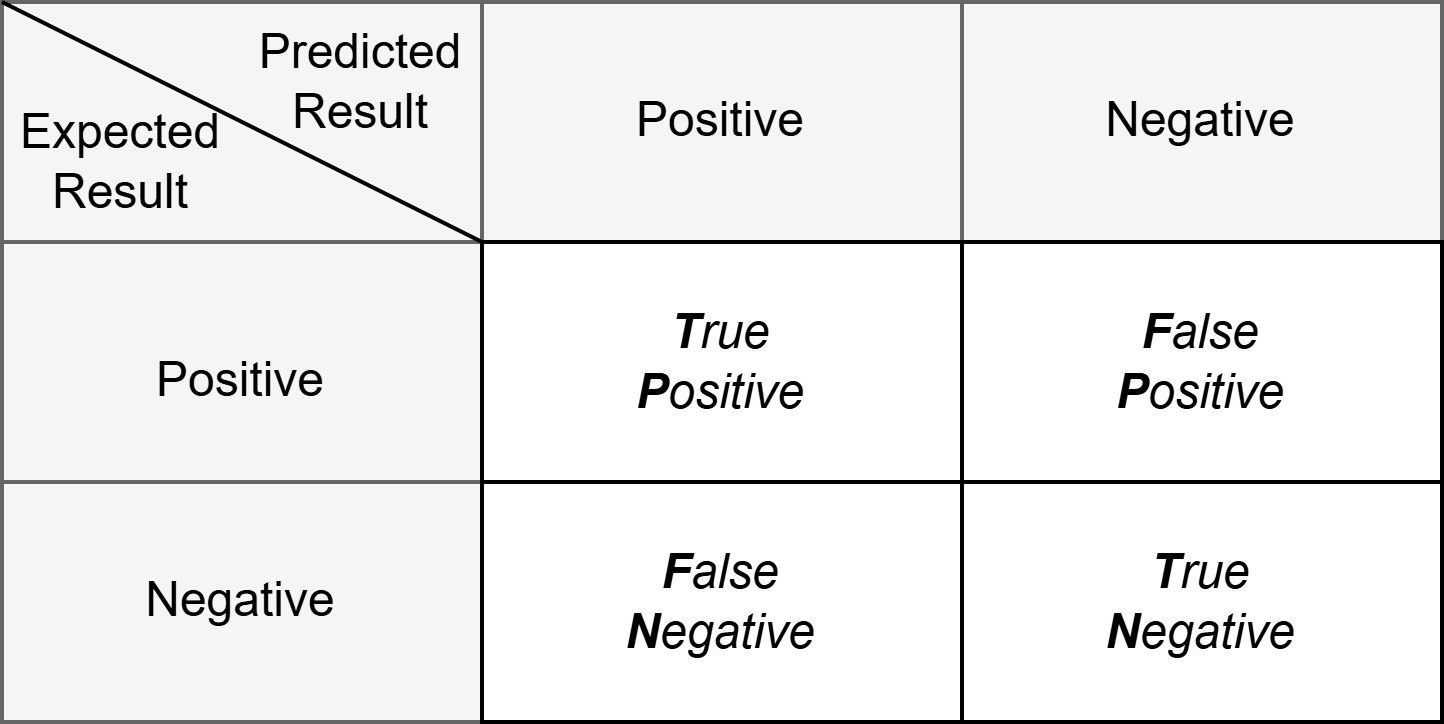
\includegraphics[scale=0.9]{confusion.png}
\caption{Confusion matrix}
\label{fig:confusion}
\centering
\end{figure}
The confusion matrix has the following outcomes:
		\begin{itemize}
			\item \textit{true positive}, if the expected result is positive and the predicted result is also positive.
			\item \textit{false positive}, if the expected result is positive but the predicted result is negative.
			\item \textit{false negative}, if the expected result is negative but the predicted result is positive.
			\item \textit{true negative}, if the expected result is negative and the predicted result is also negative.
		\end{itemize}


\textit{Precision-recall}


Precision is the ratio of True Positives to all the positives of the result set.

\begin{equation}
 precision = \frac{TP}{TP+FN}
\end{equation}
The recall is the ratio of True Positives to all the positives of the reference set.

\begin{equation}
 recall = \frac{TP}{TP+FP}
\end{equation}

As mentioned in section \ref{sec:definition}, to distinguish the key classes from the rest of the classes a TOP threshold is used. Some researchers consider that 15\% of the total classes is the best value for the TOP threshold and others consider that the value should be in the range of 20-30. 

The precision-recall metric is suited if the threshold value is fixed. If the threshold value is variable, then metrics that capture the behavior over all possible values must be used. Such metric is the Receiver Operating Characteristic metric.

\textit{Receiver Operating Characteristic Area Under Curve}


The ROC graph is a two-dimensional graph that has on the X-axis plotted the false positive rate and on the Y-axis the true positive rate. By plotting the true positive rate and the false positive rate at thresholds that vary between a minimum and a maximum possible value we obtain the ROC curve. The area under the ROC curve is called Area Under the Curve (AUC).

The true positive rate of a classifier is calculated as the division between the number of true positive results identified and all the positive results identified:

\begin{equation}
 True\ positive\ rate (TPR) = \frac{TP}{TP+FN}
\end{equation}
The false positive rate of a classifier is calculated as the division between the number of false positive results identified and all the negative results identified:

\begin{equation}
 False\ positive\ rate (FPR) = \frac{FP}{FP+TN}
\end{equation}


In multiple related works, the ROC-AUC metric has been used to evaluate the results for finding key classes of software systems.
For a classifier to be considered good, its ROC-AUC metric value should be as close to 1 as possible, when the value is 1 then the classifier is considered to be perfect.

Osman et al. obtained in their research an average Area Under the Receiver Operating Characteristic Curve (ROC-AUC) score of 0.750 \cite{6676885}. Thung et al. obtained an average ROC-AUC score of 0.825 \cite{rocclasification}  and Sora et al. obtained an average ROC-AUC score of 0.894 \cite{Finding-key-classes}.

\section{Baseline approach}
\label{sec:previous_measurements}

We use the research of I. Sora et al \cite{Finding-key-classes} as a baseline for our research involving the usage of logical dependencies to find key classes. 
The baseline approach uses a tool that takes as an input the source code of the system and applies ranking strategies to rank the classes according to their importance. 

In order to rank the classes according to their importance, different class metrics are used \cite{Ding2016AnIA}, \cite{ZaidmanJurnal}, \cite{PAN2018188}. Below are presented some of the class metrics used in the baseline approach in order to rank the classes according to their importance.



\subsubsection{Class attributes that characterize key classes}
The metrics used in the baseline research can be grouped into the following categories: 

\begin{itemize}
	\item class size metrics: number of fields (NoF),  number of methods (NoM), global size (Size = NoF+NoM).
	\item class connection metrics, any structural dependency between two classes:
		\begin{itemize}
			\item CONN-IN, the number of distinct classes that use a class;
			\item CONN-OUT, the total number of distinct classes that are used by a class;
			\item CONN-TOTAL, the total number of distinct classes that a class uses or are used by a class (CONN-IN + CONN-OUT).
			\item CONN-IN-W, the total weight of distinct classes that use a class. 
			\item CONN-OUT-W, the total weight of distinct classes that are used by a class. 
			\item CONN-TOTAL-W, the total weight of all connections of the class (CONN-IN-W + CONN-OUT-W) \cite{Finding-key-classes}.
		\end{itemize}
	\item class pagerank values, previous research use pagerank values computed on both directed and undirected, weighted and unweighted graphs:
		\begin{itemize}
			\item PR - value computed on the directed and unweighted graph;
			\item PR-W - value computed on the directed and weighted graph;
			\item PR-U - value computed on the undirected and unweighted graph;
			\item PR-U-W - value computed on the undirected and weighted graph;
			\item PR-U2-W - value computed on the weighted graph with back-recommendations \cite{PagerankENASE}, \cite{enase15}, \cite{Finding-key-classes}, \cite{PagerankSACI}.
		\end{itemize}
\end{itemize}


Based on the class attributes presented, all the classes of the system are ranked. To differentiate the important (key) classes from the rest of the classes, a TOP threshold for the top classes found is set. 
The threshold vary between 20 and 30 classes.



The baseline approach not only identifies the key classes but also evaluates the performance of the solution produced. 
The same approach as the one presented in section \ref{sec:evalmetrics} is used for the evaluation of the results. The key classes found by the ranking algorithm are compared with a reference solution that is extracted from the developer documentation by using a classification model.

The true positives (TP) are the classes found in the reference solution and also in the top TOP ranked classes. False positives (FP) are the classes that are not in the reference solution but are in the TOP ranked classes.
True Negatives (TN) are classes that are found neither in the reference solution nor in the TOP ranked classes. False Negatives (FN) are classes that are found in the reference solution but not found in the TOP ranked classes.


Due to the fact that the TOP threshold is varied, the Receiver Operating Characteristic Area Under Curve metric is used for the evaluation of the results.

The entire workflow of the baseline approach that was presented above is also presented in figure \ref{fig:baseline_approach}.

\begin{figure}[H]
\centering
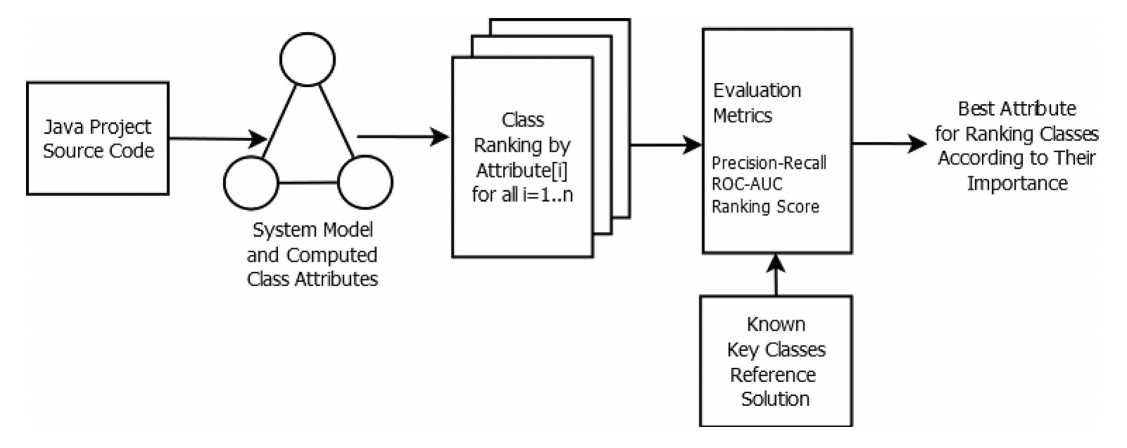
\includegraphics[width=\textwidth]{baseline_approach.PNG}
\caption{Overview of the baseline approach. Reprinted from “Finding key classes in object-oriented
software systems by techniques based on static analysis.” by Ioana Sora and Ciprian-Bogdan Chirila, 2019, Information and Software Technology, 116:106176. Reprinted with permission. }
\label{fig:baseline_approach}
\centering
\end{figure}


\chapter{Key classes detection using logical dependencies}
\label{cap:usage}

\section{Data set used}
\label{sec:dataset}
In this section, we will look over all the systems studied in the baseline research presented in section \ref{sec:previous_measurements}, and we will try to identify the systems that could be used also in our current research involving logical dependencies.


The research of I. Sora et al \cite{Finding-key-classes} takes into consideration structural public dependencies that are extracted using static analysis techniques and was performed on the object-oriented systems presented in table \ref{tab:keyclass:overview}.

The requirements for a system to qualify as suited for investigations using logical dependencies are: has to be on GitHub, has to have release tags to identify the version, and also has to have an increased number of commits. 
From the total of 14 object-oriented systems listed in the paper \cite{Finding-key-classes}, 13 of them have repositories in Github \ref{tab:gitfoundsystems}. And from the found repositories we identified only 6 repositories that have the same release tag as the specified version from table \ref{tab:keyclass:overview}. It is important to identify the correct release tag for each repository to limit the commits further analyzed by date. Only commits that were made until the specified release are considered and analyzed.
The commits number found on the remaining 6 repositories varies from 19108 commits for Tomcat Catalina to 149 commits for JHotDraw. In order to have more accurate results, we need a significant number of commits, so we reached the conclusion that only 3 systems can be used for key classes detection using logical dependencies: Apache Ant, Hibernate, and Tomcat Catalina.  From all the systems mentioned in table \ref{tab:keyclass:overview} Apache Ant is the most used and analyzed in other  works \cite{enase19}, \cite{7332515}, \cite{1402122}, \cite{Kamran2016IdentificationOC}.

\begin{table}[H]
\renewcommand{\arraystretch}{1}
\caption{Analyzed software systems in previous research paper.}
\label{tab:keyclass:overview}
\centering
\resizebox{\textwidth}{!}{
\begin{tabular}{|c|c|p{7cm}|c|}
\hline
ID	&	System	&	Description	&	Version	\\
\hline
Sl	&	Apache Ant	&	Java library and command line tool that drive the build processes as targets and extension points depending upon each other	&	1.6.1	\\ \hline
S2	&	Argo UML	&	UML modelling tool with support for all UML diagrams.	&	0.9.5	\\ \hline
S3	&	GWT Portlets	&	Open source web framework for building GWT (Google Web Toolkit) Applications.	&	0.9.5 beta	\\ \hline
S4	&	Hibernate 	&	Persistence framework for Java.	&	5.2.12	\\ \hline
S5	&	javaclient	&	Java distributed application for playing with robots	&	2.0.0	\\ \hline
S6	&	jEdit	&	Java mature text editor for programmers.	&	5.1.0	\\ \hline
S7	&	JGAP	&	Genetic Algorithms and Genetic Programming Java library.	&	3.6.3	\\ \hline
S8	&	JHotDraw	&	JHotDraw is a two-dimensional graphics framework for structured drawing editors that is written in Java.	&	6.0b.1	\\ \hline
S9	&	JMeter	&	JMeter is a Java application designed to load test functional behavior and measure performance	&	2.0.1	\\ \hline
S10	&	Log4j	&	Logging Service	&	2.10.0	\\ \hline
S11	&	Mars	&	The Mars Simulation Project is a Java project that models and simulates human settlements on Mars planet	&	3.06.0	\\ \hline
S12	&	Maze	&	The Maze-solver project simulates an artificial intelligence algorithm on a maze	&	1.0.0	\\ \hline
S13	&	Neuroph	&	Neuroph is a Java neural network framework.	&	2.2.0	\\ \hline
S14	&	Tomcat Catalina	&	The Apache Tomcat project is an open-source implementation of JavaServlet and JavaServerPages technologies	&	9.0.4	\\ \hline
S15	&	Wro4J	&	The Wro4J is a web resource (JS and CSS) optimizer for Java.	&	1.6.3	\\ 
\hline
\end{tabular}
}
\end{table}



\begin{table}[H]
\renewcommand{\arraystretch}{1}
\caption{Found systems and versions of the systems in GitHub. }
\label{tab:gitfoundsystems}
\centering
\scalebox{0.8}{
\begin{tabular}{|c|c|c|c|c|}
\hline
ID	&	System	&	Version	&	Release Tag name	&	Commits number	\\
\hline
\rowcolor{lightgreen}
Sl	&	Apache Ant	&	1.6.1	&	rel/1.6.1	&	6713	\\
S2	&	Argo UML	&	0.9.5	&	not found	&	0	\\
S3	&	GWT Portlets	&	0.9.5 beta	&	not found	&	0	\\
\rowcolor{lightgreen}
S4	&	Hibernate 	&	5.2.12	&	5.2.12	&	6733	\\
S5	&	javaclient	&	2.0.0	&	not found	&	0	\\
S6	&	jEdit	&	5.1.0	&	not found	&	0	\\
S7	&	JGAP	&	3.6.3	&	not found	&	0	\\
S8	&	JHotDraw	&	6.0b.1	&	not found	&	149	\\
S9	&	JMeter	&	2.0.1	&	v2\_1\_1	&	2506	\\
S10	&	Log4j	&	2.10.0	&	v1\_2\_10-recalled	&	634	\\
S11	&	Mars	&	3.06.0	&	not found	&	0	\\
S12	&	Maze	&	1.0.0	&	not found	&	0	\\
S13	&	Neuroph	&	2.2.0	&	not found	&	0	\\
\rowcolor{lightgreen}
S14	&	Tomcat Catalina	&	9.0.4	&	9.0.4	&	19108	\\
S15	&	Wro4J	&	1.6.3	&	v1.6.3	&	2871	\\
\hline
\end{tabular}
}
\end{table}



\section{Measurements using logical dependencies}
\label{sec:current_measurements}

As we mentioned in the beginning the purpose is to check if the logical dependencies can improve key class detection. 

As presented in section \ref{sec:previous_measurements}, and section \ref{sec:definition} the key class detection was done by using structural dependencies of the system. 
In this section, we will use the same tool used in the baseline approach presented in section \ref{sec:previous_measurements}, and we will add a new input to it, the logical dependencies. 

Below is a comparison between the new approach and baseline approach, how we collect the logical dependencies, the results obtained previously, and the new results obtained. 
The new results are separated into two categories, the results obtained by using structural and logical dependencies and the results obtained by using only logical dependencies. 



\subsection{Comparison with the baseline approach}
\label{sec:comparison}

The baseline approach uses a tool that takes as input the source code of the system to identify the key classes and the reference solution to evaluate the quality of the solution. 
We modified the tool such that it can also take as input the logical dependencies. 

In order to rank the classes according to their importance, the tool uses different class metrics. The list of the metrics used in the baseline approach is presented in section \ref{sec:previous_measurements}.  
The difference in the metrics used compared with the baseline approach is that we use a subset of those metrics. The reason why we are not using all the metrics is that the extracted logical dependencies are undirected. The metrics used by the current approach are CONN-TOTAL, CONN-TOTAL-W, PR-U, PR-U-W, and PR-U2-W.

We did not change the rest of the workflow of the tool. Meaning that the TOP threshold is varied between 20 and 30 and the resulting solution is evaluated by using the ROC-AUC metric. The goal being a ROC-AUC (Receiver Operating Characteristic - Area Under the Curve) metric value as close to 1 as possible.

\begin{figure}[H]
\centering
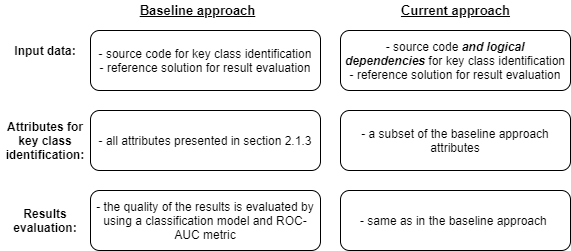
\includegraphics[width=\textwidth]{baseline_comparison.png}
\caption{ Comparison between the new approach and the baseline }
\label{fig:baseline_comparison}
\centering
\end{figure}

\subsection{Logical dependencies collection and current workflow used}

The logical dependencies are those co-changing pairs extracted from the versioning system history that remain after filtering. The filtering part consists of applying two filters: the filter based on commit size and the filter based on connection strength. 

To determine the connection strength of a pair, we first need to calculate the connection factors for both entities that form a co-changing pair.
Assuming that we have a co-changing pair formed by entities A and B, the connection factor of entity A with entity B is the percentage from the total commits involving A that contains entity B. The connection factor of entity B with entity A is the percentage from the total commits involving B that contain also entity A.

\begin{equation}
 connection\ factor\ for\ A = \frac{100 * commits\ involving\ A\ and\ B}{total\ nr\ of\ commits\ involving\ A}
\end{equation}

\begin{equation}
 connection\ factor\ for\ B = \frac{100 * commits\ involving\ A\ and\ B}{total\ nr\ of\ commits\ involving\ B}
\end{equation}

We calculated the connection factor for each entity involved in a co-changing pair and filtered the co-changing pairs based on it. The rule set is that both entities had to have a connection factor with each other greater than the threshold value.

After the filtering part, the remaining co-changing pairs, now called logical dependencies, are exported in CSV files.

The entire process of extracting co-changing pairs from the versioning system, filter them, and export the remaining ones into CSV files is done with a tool written in Python.

The next step is to use the exported logical dependencies for key classes detection. In order to do that we used the same key class detection tool used in the previous research presented in section \ref{sec:previous_measurements}. We adapted the tool to be able to process also logical dependencies because previously the tool used only structural dependencies extracted from the source code of the software systems. 
The workflow is presented in figure \ref{fig:workflow_key}

\begin{figure}[H]
\centering
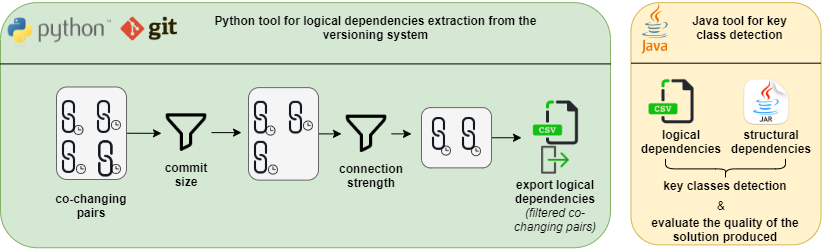
\includegraphics[width=\textwidth]{key_class_workflow.png}
\caption{Workflow for key classes detection}
\label{fig:workflow_key}
\centering
\end{figure}


\subsection{Measurements using only the baseline approach}


In table \ref{tab:previousresults} are presented the ROC-AUC values for different attributes computed for the systems Ant, Tomcat Catalina, and Hibernate by using the baseline approach. We intend to compare these values with the new values obtained by using also logical dependencies in key class detection.

\begin{table}[!h]
\renewcommand{\arraystretch}{1}
\caption{ROC-AUC metric values extracted. }
\label{tab:previousresults}
\centering
\scalebox{0.9}{
\begin{tabular}{|c|ccc|}
\hline
Metrics &	Ant	&	Tomcat Catalina	&	Hibernate	\\
\hline

PR\_U2\_W	&	0.95823	&	0.92341	&	0.95823	\\
PR	&	0.94944	&	0.92670	&	0.94944	\\
PR\_U	&	0.95060	&	0.93220	&	0.95060	\\
CONN\_TOTAL\_W	&	0.94437	&	0.92595	&	0.94437	\\
CONN\_TOTAL	&	0.94630	&	0.93903	&	0.94630	\\

\hline
\end{tabular}
}
\end{table}





\subsection{Measurements using combined structural and logical dependencies}

The tool used in the baseline approach runs a graph-ranking algorithm. 
The graph used contains the structural dependencies extracted from static source code analysis.
Each edge in the graph represents a dependency, the entities that form a structural dependency are represented as vertices in the graph. 
As mentioned in section \ref{sec:comparison}, we modified the tool to read also logical dependencies and add them to the graph. 
In this section, we add in the graph the logical dependencies together with the structural dependencies. 

In tables \ref{tab:measurementscombined:ant}, \ref{tab:measurementscombined:tomcat}, and \ref{tab:measurementscombined:hibernate}, on each line, we have the metric that is calculated and on each column, we have the connection strength threshold that was applied to the logical dependencies used in identifying the key classes.
We started with logical dependencies that have a connection strength greater than 10\%, which means that in at least 10\% of the commits involving A or B, A and B update together. Then we increased the threshold value by 10 until we remained only with entities that update in all the commits together. The last column contains the results obtained previously by the tool by only using structural dependencies.

As for the new results obtained by combining structural and logical dependencies, highlighted with orange are the values that are close to the previously registered values but did not surpass them. Highlighted with green are values that are better than the previously registered values. At this step, we can also observe that for all three systems measured in tables \ref{tab:measurementscombined:ant}, \ref{tab:measurementscombined:tomcat}, and \ref{tab:measurementscombined:hibernate}, the best values obtained are for connection strength between 40-70\%.

\begin{table}[!h]
\renewcommand{\arraystretch}{1}
\caption{Measurements for Ant using structural and logical dependencies combined}
\label{tab:measurementscombined:ant}
\centering
\scalebox{0.7}{
\begin{tabular}{|c|cccccccccc|c|}
\hline
Metrics &	$\geq10\%$	&	$\geq20\%$		&	$\geq30\%$		&	$\geq40\%$		&	$\geq50\%$		&	$\geq60\%$		&	$\geq70\%$		&	$\geq80\%$		&	$\geq90\%$		&	$\geq100\%$		&	Baseline \\
\hline

PR\_U2\_W	&	0.924	&	0.925	&	0.926	&	0.927	&	0.927	&	0.927	&	\cellcolor{lightgreen}0.929	&	0.928	&	0.928	&	0.928	&	0.929	\\
PR	&	0.914	&	0.854	&	0.851	&	\cellcolor{lightgreen}0.866	&	\cellcolor{lightgreen}0.876	&	\cellcolor{lightgreen}0.882	&	\cellcolor{lightgreen}0.887	&	0.854	&	0.852	&	0.852	&	0.855	\\
PR\_U	&	0.910	&	0.930	&	0.933	&	0.933	&	\cellcolor{lightgreen}0.935	&	\cellcolor{lightgreen}0.934	&	\cellcolor{lightgreen}0.939	&	0.933	&	0.933	&	0.933	&	0.933	\\
CON\_T\_W	&	0.924	&	0.928	&	0.931	&	0.932	&	0.933	&	0.934	&	\cellcolor{lightgreen}0.936	&	0.934	&	0.934	&	0.934	&	0.934	\\
CON\_T	&	0.840	&	0.886	&	0.904	&	0.909	&	0.915	&	0.923	&	0.932	&	0.935	&	\cellcolor{lightorange}0.936	&	\cellcolor{lightorange}0.936	&	0.942	\\

\hline
\end{tabular}
}
\end{table}


\begin{table}[!h]
\renewcommand{\arraystretch}{1}
\caption{Measurements for Tomcat using structural and logical dependencies combined}
\label{tab:measurementscombined:tomcat}
\centering
\scalebox{0.7}{
\begin{tabular}{|c|cccccccccc|c|}
\hline
Metrics &	$\geq10\%$	&	$\geq20\%$		&	$\geq30\%$		&	$\geq40\%$		&	$\geq50\%$		&	$\geq60\%$		&	$\geq70\%$		&	$\geq80\%$		&	$\geq90\%$		&	$\geq100\%$		&	Baseline \\
\hline

PR\_U2\_W	&	0.910	&	0.917	&	0.923	&	\cellcolor{lightgreen}0.924	&	\cellcolor{lightgreen}0.924	&	\cellcolor{lightgreen}0.924	&	\cellcolor{lightgreen}0.924	&	\cellcolor{lightgreen}0.924	&	\cellcolor{lightgreen}0.924	&	\cellcolor{lightgreen}0.924	&	0.923	\\
PR	&	0.811	&	0.800	&	0.815	&	0.834	&	0.847	&	0.852	&	0.853	&	0.858	&	0.858	&	0.858	&	0.927	\\
PR\_U	&	0.910	&	0.921	&	0.931	&	\cellcolor{lightgreen}0.933	&	\cellcolor{lightgreen}0.933	&	0.932	&	\cellcolor{lightgreen}0.933	&	0.932	&	0.932	&	0.932	&	0.932	\\
CON\_T\_W	&	0.914	&	0.920	&	0.924	&	\cellcolor{lightorange}0.926	&	0.926	&	0.926	&	0.926	&	0.926	&	0.926	&	0.926	&	0.926	\\
CON\_T	&	0.868	&	0.906	&	0.930	&	0.936	&	0.937	&	\cellcolor{lightorange}0.938	&	0.938	&	0.938	&	0.938	&	0.938	&	0.939	\\
																												

\hline
\end{tabular}
}
\end{table}


\begin{table}[!h]
\renewcommand{\arraystretch}{1}
\caption{Measurements for Hibernate using structural and logical dependencies combined}
\label{tab:measurementscombined:hibernate}
\centering
\scalebox{0.7}{
\begin{tabular}{|c|cccccccccc|c|}
\hline
Metrics &	$\geq10\%$	&	$\geq20\%$		&	$\geq30\%$		&	$\geq40\%$		&	$\geq50\%$		&	$\geq60\%$		&	$\geq70\%$		&	$\geq80\%$		&	$\geq90\%$		&	$\geq100\%$		&	Baseline \\
\hline

PR\_U2\_W	&	0.954	&	0.957	&	\cellcolor{lightorange}0.958	&	0.958	&	0.958	&	0.958	&	0.958	&	0.958	&	0.958	&	0.958	&	0.958	\\
PR	&	0.929	&	0.929	&	0.933	&	0.939	&	0.939	&	0.946	&	\cellcolor{lightorange}0.947	&	0.947	&	0.947	&	0.947	&	0.949	\\
PR\_U	&	0.942	&	0.947	&	0.948	&	0.949	&	0.949	&	\cellcolor{lightorange}0.950	&	0.950	&	0.950	&	0.950	&	0.950	&	0.951	\\
CON\_T\_W	&	0.939	&	0.942	&	0.943	&	0.944	&	0.944	&	\cellcolor{lightgreen}0.945	&	\cellcolor{lightgreen}0.945	&	\cellcolor{lightgreen}0.945	&	\cellcolor{lightgreen}0.945	&	\cellcolor{lightgreen}0.945	&	0.944	\\
CON\_T	&	0.924	&	0.933	&	0.938	&	0.941	&	0.941	&	0.944	&	\cellcolor{lightorange}0.945	&	0.945	&	0.945	&	0.945	&	0.946	\\


\hline
\end{tabular}
}
\end{table}





\subsection{Measurements using only logical dependencies}
In the previous section, we added in the graph based on which the ranking algorithm works the logical and structural dependencies. In the current section, we will add only the logical dependencies to the graph.

In tables \ref{tab:measurementshistory:ant}, \ref{tab:measurementshistory:tomcat}, and \ref{tab:measurementshistory:hibernate}, are presented the results obtained by using only logical dependencies to detect key classes. The measurements obtained are not as good as using logical and structural dependencies combined or using only structural dependencies. But, all the values obtained are above 0.5, which means that a good part of the key classes is detected by only using logical dependencies.  As mentioned in section \ref{sec:evalmetrics}, a classifier is good if it has the ROC-AUC value as close to 1 as possible. 


One possible explanation for the less performing results is that the key classes may have a better design than the rest of the classes, which means that are less prone to change. If the key classes are less prone to change, this implies that the number of dependencies extracted from the versioning system can be less than for other classes.

\begin{table}[!h]
\renewcommand{\arraystretch}{1}
\caption{Measurements for Ant using only logical dependencies}
\label{tab:measurementshistory:ant}
\centering
\scalebox{0.7}{
\begin{tabular}{|c|cccccccccc|c|}
\hline
Metrics &	$\geq10\%$	&	$\geq20\%$		&	$\geq30\%$		&	$\geq40\%$		&	$\geq50\%$		&	$\geq60\%$		&	$\geq70\%$		&	$\geq80\%$		&	$\geq90\%$		&	$\geq100\%$		&	Baseline \\
\hline

PR\_U2\_W	&	0.720	&	0.627	&	0.718	&	0.703	&	0.732	&	0.824	&	0.852	&	\cellcolor{lightorange}0.881	&	0.876	&	0.876	&	0.929	\\
PR	&	0.720	&	0.627	&	0.718	&	0.703	&	0.732	&	0.824	&	0.852	&	\cellcolor{lightorange}0.881	&	0.876	&	0.876	&	0.855	\\
PR\_U	&	0.720	&	0.627	&	0.718	&	0.703	&	0.732	&	0.824	&	0.852	&	\cellcolor{lightorange}0.881	&	0.876	&	0.876	&	0.933	\\
CON\_T\_W	&	0.722	&	0.581	&	0.644	&	0.676	&	0.727	&	0.819	&	0.842	&	0.874	&	\cellcolor{lightorange}0.876	&	0.876	&	0.934	\\
CON\_T	&	0.722	&	0.581	&	0.644	&	0.676	&	0.727	&	0.819	&	0.842	&	0.874	&	\cellcolor{lightorange}0.876	&	0.876	&	0.942	\\

\hline
\end{tabular}
}
\end{table}


\begin{table}[!h]
\renewcommand{\arraystretch}{1}
\caption{Measurements for Tomcat using only logical dependencies}
\label{tab:measurementshistory:tomcat}
\centering
\scalebox{0.8}{
\begin{tabular}{|c|cccccccccc|c|}
\hline
Metrics &	$\geq10\%$	&	$\geq20\%$		&	$\geq30\%$		&	$\geq40\%$		&	$\geq50\%$		&	$\geq60\%$		&	$\geq70\%$		&	$\geq80\%$		&	$\geq90\%$		&	$\geq100\%$		&	Previous \\
\hline

PR\_U2\_W	&	0.672	&	0.656	&	0.645	&	0.697	&	0.754	&	0.776	&	0.786	&	\cellcolor{lightorange}0.799	&	0.799	&	0.799	&	0.923	\\
PR	&	0.685	&	0.643	&	0.642	&	0.697	&	0.754	&	0.776	&	0.786	&	\cellcolor{lightorange}0.799	&	0.799	&	0.799	&	0.927	\\
PR\_U	&	0.685	&	0.643	&	0.644	&	0.697	&	0.754	&	0.776	&	0.786	&	\cellcolor{lightorange}0.799	&	0.799	&	0.799	&	0.932	\\
CON\_T\_W	&	0.694	&	0.636	&	0.636	&	0.697	&	0.754	&	0.776	&	0.786	&	\cellcolor{lightorange}0.799	&	0.799	&	0.799	&	0.926	\\
CON\_T	&	0.654	&	0.611	&	0.636	&	0.697	&	0.754	&	0.776	&	0.786	&	\cellcolor{lightorange}0.799	&	0.799	&	0.799	&	0.939	\\

				
\hline
\end{tabular}
}
\end{table}


\begin{table}[!h]
\renewcommand{\arraystretch}{1}
\caption{Measurements for Hibernate using only logical dependencies}
\label{tab:measurementshistory:hibernate}
\centering
\scalebox{0.8}{
\begin{tabular}{|c|cccccccccc|c|}
\hline
Metrics &	$\geq10\%$	&	$\geq20\%$		&	$\geq30\%$		&	$\geq40\%$		&	$\geq50\%$		&	$\geq60\%$		&	$\geq70\%$		&	$\geq80\%$		&	$\geq90\%$		&	$\geq100\%$		&	Baseline \\
\hline

PR\_U2\_W	&	0.657	&	0.564	&	0.601	&	0.619	&	0.622	&	0.650	&	0.653	&	\cellcolor{lightorange}0.654	&	0.654	&	0.654	&	0.958	\\
PR	&	0.644	&	0.564	&	0.601	&	0.619	&	0.622	&	0.650	&	0.653	&	\cellcolor{lightorange}0.654	&	0.654	&	0.654	&	0.949	\\
PR\_U	&	0.644	&	0.564	&	0.601	&	0.619	&	0.622	&	0.650	&	0.653	&	\cellcolor{lightorange}0.654	&	0.654	&	0.654	&	0.951	\\
CON\_T\_W	&	0.649	&	0.564	&	0.601	&	0.619	&	0.622	&	0.650	&	0.653	&	\cellcolor{lightorange}0.654	&	0.654	&	0.654	&	0.944	\\
CON\_T	&	0.644	&	0.564	&	0.601	&	0.619	&	0.622	&	0.650	&	0.653	&	\cellcolor{lightorange}0.654	&	0.654	&	0.654	&	0.946	\\


\hline
\end{tabular}
}
\end{table}

\section{Correlation between details of the systems and results}
\label{sec:overlapping}

In this section, we discuss about the correlation between the details of the systems and the results obtained in section \ref{sec:current_measurements}.

The reason why we are doing this correlation is to find if there are some links between the details of the systems and the results obtained. 

The results obtained are presented in figures \ref{fig:plot_sd_ld_ant} - \ref{fig:plot_ld_hibernate}. We are using plots to display the results obtained to have a clearer view of how the results fluctuate over different thresholds values.




\begin{figure}[H]
\centering
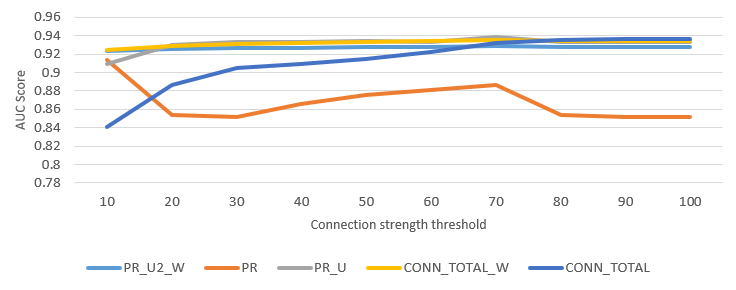
\includegraphics[width=\textwidth]{ant_SD_LD.PNG}
\caption{Variation of AUC score when varying connection strength threshold for Ant. Results for structural and logical dependencies combined. }
\label{fig:plot_sd_ld_ant}
\centering
\end{figure}


\begin{figure}[H]
\centering
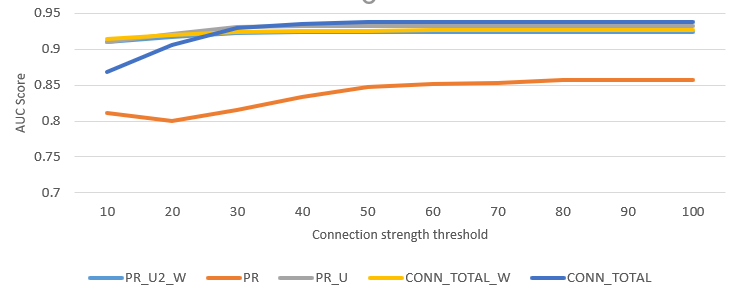
\includegraphics[width=\textwidth]{tomcat_SD_LD.PNG}
\caption{Variation of AUC score when varying connection strength threshold for Tomcat. Results for structural and logical dependencies combined. }
\label{fig:plot_sd_ld_tomcat}
\centering
\end{figure}


\begin{figure}[H]
\centering
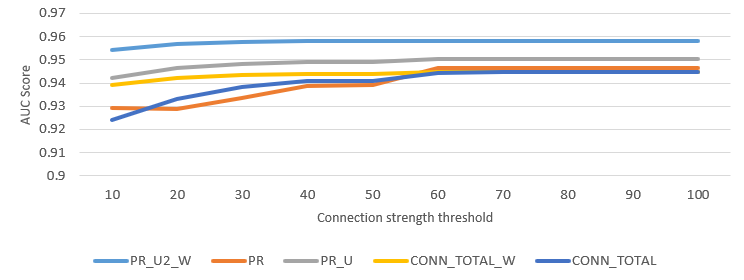
\includegraphics[width=\textwidth]{hibernate_SD_LD.PNG}
\caption{Variation of AUC score when varying connection strength threshold for Hibernate. Results for structural and logical dependencies combined. }
\label{fig:plot_sd_ld_hibernate}
\centering
\end{figure}



\begin{figure}[H]
\centering
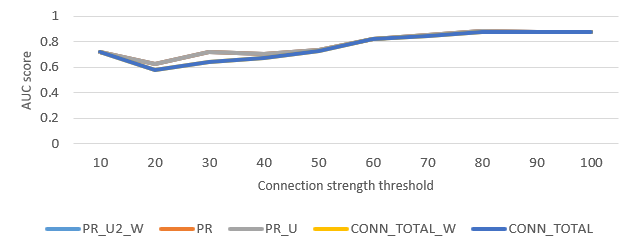
\includegraphics[width=\textwidth]{ant_LD.PNG}
\caption{Variation of AUC score when varying connection strength threshold for Ant. Results for logical dependencies only. }
\label{fig:plot_ld_ant}
\centering
\end{figure}


\begin{figure}[H]
\centering
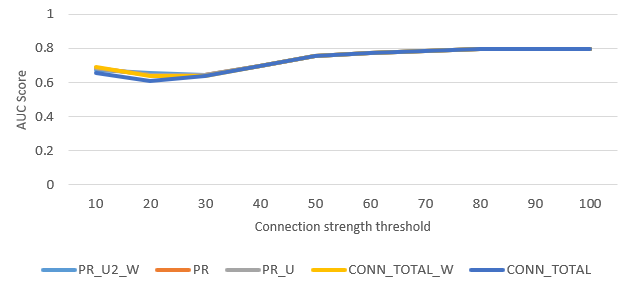
\includegraphics[width=\textwidth]{tomcat_LD.PNG}
\caption{Variation of AUC score when varying connection strength threshold for Tomcat. Results for logical dependencies only. }
\label{fig:plot_ld_tomcat}
\centering
\end{figure}


\begin{figure}[H]
\centering
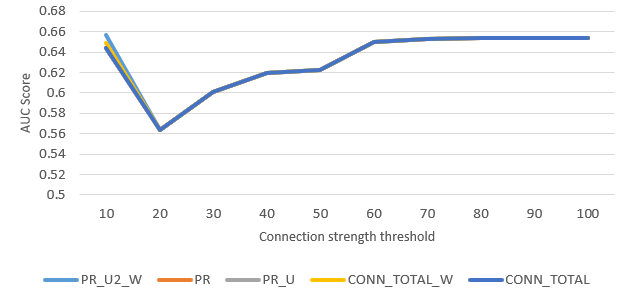
\includegraphics[width=\textwidth]{hibernate_LD.PNG}
\caption{Variation of AUC score when varying connection strength threshold for Hibernate. Results for logical dependencies only.}
\label{fig:plot_ld_hibernate}
\centering
\end{figure}


The details of the systems are presented in two tables.  In table \ref{tab:overlap} are the overlappings between structural and logical dependencies expressed in percentages. Each column represents the percentage of logical dependencies that are also structural, for each column the logical dependencies are obtained by applying a different connection strength filter. The connection strength filter begins at 10, meaning that in at least 10 \% of the total commits involving two entities, the entities update together. We increase the connection strength filter by 10 up until we reach 100, meaning that in all the commits that involve one entity, the other entity is present also.


In table \ref{tab:ratio_sd_ld} are the ratio numbers between structural dependencies and logical dependencies. We added this table in order to highlight how different the total number of both dependencies is.


\begin{table}[!h]
\renewcommand{\arraystretch}{1}
\caption{Percentage of logical dependencies that are also structural dependencies}
\label{tab:overlap}
\centering
\scalebox{0.7}{
\begin{tabular}{|c|cccccccccc|}
\hline
System &	$\geq10\%$	&	$\geq20\%$		&	$\geq30\%$		&	$\geq40\%$		&	$\geq50\%$		&	$\geq60\%$		&	$\geq70\%$		&	$\geq80\%$		&	$\geq90\%$		&	$\geq100\%$ \\
\hline
Ant	&	25.202	&	34.419	&	36.385	&	34.656	&	33.528	&	33.333	&	28.659	&	33.333	&	35.294	&	35.294	\\
Tomcat Catalina	&	4.059	&	22.089	&	25.000	&	25.758	&	25.926	&	37.525	&	47.368	&	55.285	&	75.000	&	76.923	\\
Hibernate	&	6.546	&	26.607	&	29.565	&	32.374	&	32.543	&	45.170	&	44.980	&	42.473	&	42.473	&	42.473	\\
\hline
\end{tabular}
}
\end{table}



\begin{table}[!h]
\renewcommand{\arraystretch}{1}
\caption{Ratio between structural and logical dependencies (SD/LD)}
\label{tab:ratio_sd_ld}
\centering
\scalebox{0.7}{
\begin{tabular}{|c|cccccccccc|}
\hline
System &	$\geq10\%$	&	$\geq20\%$		&	$\geq30\%$		&	$\geq40\%$		&	$\geq50\%$		&	$\geq60\%$		&	$\geq70\%$		&	$\geq80\%$		&	$\geq90\%$		&	$\geq100\%$ \\
\hline
Ant	&	1.315	&	3.284	&	4.972	&	5.603	&	6.175	&	10.697	&	12.915	&	27.154	&	41.529	&	41.529	\\
Tomcat Catalina	&	0.120	&	0.923	&	1.313	&	1.531	&	1.619	&	3.177	&	7.092	&	13.146	&	67.375	&	124.385	\\
Hibernate	&	1.037	&	6.391	&	10.037	&	14.947	&	18.940	&	54.248	&	83.442	&	111.704	&	111.704	&	111.704	\\

\hline
\end{tabular}
}
\end{table}

In figures \ref{fig:plot_sd_ld_ant}, \ref{fig:plot_sd_ld_tomcat} and \ref{fig:plot_sd_ld_hibernate} are the measurements obtained by using structural and logical dependencies combined. 
In all three figures, the measurements at the beginning are smaller than the rest. Once with the increasing of the threshold value also the measurements begin to increase. Meaning that better results for key class detection are found. 
The best measurements are when the threshold value is between 40 and 60, after that, the measurements tend to decrease a little bit and stay at that fixed value. 

A possible explanation of the results fluctuation and then capping is that if we are looking at table \ref{tab:ratio_sd_ld} we can see that at the beginning, the total number of logical dependencies used is close to the number of existing structural dependencies. The high volume of logical dependencies introduced might cause an erroneous detection of the key classes, in consequence, smaller measurements. 
When the threshold begins to be more restrictive and the total number of logical dependencies used begins to decrease, the key classes detection starts to improve. This improvement stops after the threshold value reaches 60\%. If we look again at table \ref{tab:ratio_sd_ld} we can see that after 60\% the number of structural dependencies outnumbers the number of logical dependencies up to 124 times in some cases. In addition, if we look at table \ref{tab:overlap} we can see that the remaining logical dependencies overlap a lot with the structural dependencies, so we are not introducing too much new information.

 So, the number of logical dependencies used is so small that it doesn't influence the key class identification. Since the structural dependencies used don't change, we obtain the same results for different threshold values. 



In figures \ref{fig:plot_ld_ant}, \ref{fig:plot_ld_tomcat} and \ref{fig:plot_ld_hibernate} are the measurements obtained by using only logical dependencies.
Initially, we expected to see a Gaussian curve, but instead, we see a bell curve.  We think that in the beginning, we use a high number of logical dependencies in key class detection, among those logical dependencies is an important number of key classes and also an important number of other classes. But the number of other classes does not influence the key classes detection. When we start to increase the value of the threshold and filter more the logical dependencies, we also filter some of the initial detected key classes and remain with a significant number of other classes. In this case, the other classes that remain influence the measurements, causing the worst-performing solutions. 
Some of the key classes are strongly connected in the versioning system, and even for higher threshold values don't get filtered out. Meanwhile, the rest of the classes that are not key classes get filtered out for higher threshold values which leads to better performing measurements when the threshold value are above 60\%. 



\section{Comparison of the extracted data with fan-in and fan-out metric}
\label{sec:metrics}

Fan-in and fan-out are coupling metrics. The fan-in of entity A is the total number of entities that call functions of A. The fan-out of A is the total number of entities called by A \cite{5507329}.


In tables \ref{tab:measurementsfan:ant}, \ref{tab:measurementsfan:catalina}, and \ref{tab:measurementsfan:hibernate} we can find the metrics detalis for each documented key class of each system.
The first column represents the name of each key class, the second column represents the fan\_in values for each key class, the third column represents the fan\_out values, the fourth column represents the number of entities that call functions of that key class plus the number of entities that are called by the key class (fan\_in and fan\_out combined), and the fifth column represents the number of logical dependencies in which an entity is involved. 

For Ant, we can see in table \ref{tab:measurementsfan:ant} that all the key classes have logical dependencies with other classes. The LD\_NUMBER means the number of logical dependencies of an entity. The key classes with the most LD number are Project and IntrospectionHelper, these two entities can be found also in table \ref{tab:measurementstop:ant} in which we did a top 10 entities that have a logical dependency with other entities. This means that some key classes are involved in software change quite often and can be observed via system history.

\begin{table}[!h]
\renewcommand{\arraystretch}{1}
\caption{Measurements for Ant key classes}
\label{tab:measurementsfan:ant}
\centering
\scalebox{0.8}{
\begin{tabular}{|c|ccccc|}
\hline
Nr.	&	Classname	&	FAN\_IN	&	FAN\_OUT	&	FAN\_TOTAL	&	LD\_NUMBER\\
\hline
1	&	Project	&	191	&	23	&	214	&	157	\\
2	&	Target	&	28	&	6	&	34	&	78	\\
3	&	UnknownElement	&	17	&	13	&	30	&	90	\\
4	&	RuntimeConfigurable	&	17	&	13	&	30	&	118	\\
5	&	IntrospectionHelper	&	18	&	24	&	42	&	143	\\
6	&	Main	&	1	&	13	&	14	&	82	\\
7	&	TaskContainer	&	11	&	1	&	12	&	21	\\
8	&	ProjectHelper2\$ElementHandler	&	1	&	12	&	13	&	30	\\
9	&	Task	&	110	&	7	&	117	&	88	\\
10	&	ProjectHelper	&	16	&	8	&	24	&	101	\\
\hline
\end{tabular}
}
\end{table}


For Tomcat Catalina, same as for Ant, we can see in table \ref{tab:measurementsfan:catalina} that all the key classes have logical dependencies.  The key classes with the most LD number are StandardContext and Request, these two entities can also be found in table \ref{tab:measurementstop:catalina} in which we did a top 10 entities that have the most logical dependencies with other entities for Tomcat Catalina.

For Hibernate things are a little bit different, as we can see in table \ref{tab:measurementsfan:hibernate},  key classes like Criterion, Projection, or Transaction have 0 logical dependencies, meaning that those key classes are not involved in any software change. One possible explanation for this is that for Hibernate the architecture is designed in such way that the core is not often touched by change. 


\begin{table}[!h]
\renewcommand{\arraystretch}{1}
\caption{Measurements for Tomcat Catalina key classes.}
\label{tab:measurementsfan:catalina}
\centering
\scalebox{0.8}{
\begin{tabular}{|c|ccccc|}
\hline
Nr.	&	Classname	&	FAN\_IN	&	FAN\_OUT	&	FAN\_TOTAL	&	LD\_NUMBER \\
\hline
1	&	Context	&	74	&	8	&	82	&	126	\\
2	&	Request	&	48	&	28	&	76	&	215	\\
3	&	Container	&	51	&	8	&	59	&	64	\\
4	&	Response	&	38	&	12	&	50	&	90	\\
5	&	StandardContext	&	11	&	38	&	49	&	216	\\
6	&	FANector	&	23	&	9	&	32	&	89	\\
7	&	Session	&	29	&	2	&	31	&	28	\\
8	&	Valve	&	29	&	2	&	31	&	19	\\
9	&	Wrapper	&	29	&	1	&	30	&	36	\\
10	&	Manager	&	25	&	3	&	28	&	31	\\
11	&	Host	&	26	&	1	&	27	&	44	\\
12	&	Service	&	20	&	6	&	26	&	51	\\
13	&	Engine	&	23	&	2	&	25	&	1	\\
14	&	Realm	&	18	&	6	&	24	&	21	\\
15	&	CoyoteAdapter	&	1	&	22	&	23	&	140	\\
16	&	StandardHost	&	8	&	15	&	23	&	88	\\
17	&	LifecycleListener	&	21	&	1	&	22	&	3	\\
18	&    StandardEngine	&	2	&	19	&	21	&	57	\\
19	&	Pipeline	&	19	&	2	&	21	&	20	\\
20	&	Server	&	16	&	4	&	20	&	49	\\
21	&	HostConfig	&	3	&	15	&	18	&	79	\\
22	&	StandardWrapper	&	5	&	13	&	18	&	92	\\
23	&	StandardService	&	3	&	12	&	15	&	81	\\
24	&	Catalina	&	2	&	13	&	15	&	94	\\
25	&	Loader	&	14	&	1	&	15	&	18	\\
26	&	StandardServer	&	2	&	12	&	14	&	94	\\
27	&	StandardPipeline	&	1	&	10	&	11	&	62	\\
28	&	Bootstrap	&	3	&	3	&	6	&	41	\\	
\hline
\end{tabular}
}
\end{table}

\begin{table}[!h]
\renewcommand{\arraystretch}{1}
\caption{Measurements for Hibernate key classes.}
\label{tab:measurementsfan:hibernate}
\centering
\scalebox{0.8}{
\begin{tabular}{|c|ccccc|}
\hline
Nr.	&	Classname	&	FAN\_IN	&	FAN\_OUT	&	FAN\_TOTAL	&	LD\_NUMBER \\
\hline
1	&	SessionFactoryImplementor	&	438	&	43	&	481	&	51	\\
2	&	Type	&	444	&	5	&	449	&	0	\\
3	&	Table	&	89	&	29	&	118	&	82	\\
4	&	SessionImplementor	&	52	&	12	&	64	&	14	\\
5	&	Criteria	&	45	&	12	&	57	&	15	\\
6	&	Column	&	46	&	10	&	56	&	20	\\
7	&	Session	&	31	&	21	&	52	&	52	\\
8	&	Query	&	12	&	28	&	40	&	0	\\
9	&	Configuration	&	1	&	38	&	39	&	115	\\
10	&	SessionFactory	&	24	&	12	&	36	&	33	\\
11	&	Criterion	&	30	&	3	&	33	&	0	\\
12	&	Projection	&	11	&	3	&	14	&	0	\\
13	&	FANectionProvider	&	12	&	2	&	14	&	0	\\
14	&	Transaction	&	11	&	1	&	12	&	0	\\
				
\hline
\end{tabular}
}
\end{table}


%%%%%%%%%%%%%%%%%%%%%%%%%%%%%%%%%%%%%%%%%%%%%%%%%%%%%%%%%%%%%%%%%%%%%%%%%%%%%

In tables \ref{tab:measurementstop:ant}, \ref{tab:measurementstop:catalina}, and \ref{tab:measurementstop:hibernate} we can find the top 10 entities with logical dependencies. The first column represents the name of each top 10 entity, the second column represents the fan\_in values, the third column represents the fan\_out values, the fourth column represents the fan\_in and fan\_out combined, and the fifth column represents the number of logical dependencies in which the entity is involved.


We did these top 10 tables to offer an overview of the highest registered numbers for LD for each system. As we mentioned before, some of the key classes are also present in these tables, but not all of them.

In table \ref{tab:measurementstop:hibernate} we can find the top 10 measurements for Hibernate, most of the table is occupied by inner classes of AbstractEntityPersister. This is expected behavior since class AbstractEntityPersister is also present. This behavior is caused by the impossibility to separate the updates done for a class from its inner classes in the versioning system. So, each time AbstractEntityPersister records a change, also the inner classes are considered to have changed.
\begin{table}[!h]
\renewcommand{\arraystretch}{1}
\caption{Top 10 measurements for Ant. }
\label{tab:measurementstop:ant}
\centering
\scalebox{0.8}{
\begin{tabular}{|c|ccccc|}
\hline
Nr.	&	Classname	&	FAN\_IN	&	FAN\_OUT	&	FAN\_TOTAL	&	LD\_NUMBER \\
\hline
1	&	\cellcolor{lightorange}Project	&	191	&	23	&	214	&	157	\\
2	&	Project\$AntRefTable	&	1	&	2	&	3	&	157	\\
3	&	Path	&	39	&	13	&	52	&	147	\\
4	&	Path\$PathElement	&	3	&	2	&	5	&	147	\\
5	&	\cellcolor{lightorange}IntrospectionHelper	&	18	&	24	&	42	&	143	\\
6	&	IntrospectionHelper\$AttributeSetter	&	8	&	1	&	9	&	143	\\
7	&	IntrospectionHelper\$Creator	&	3	&	5	&	8	&	143	\\
8	&	IntrospectionHelper\$NestedCreator	&	7	&	1	&	8	&	143	\\
9	&	Ant	&	2	&	15	&	17	&	136	\\
10	&	Ant\$Reference	&	3	&	1	&	4	&	136	\\
\hline
\end{tabular}
}
\end{table}

\begin{table}[!h]
\renewcommand{\arraystretch}{1}
\caption{Top 10 measurements for Tomcat Catalina. }
\label{tab:measurementstop:catalina}
\centering
\scalebox{0.8}{
\begin{tabular}{|c|ccccc|}
\hline
Nr.	&	Classname	&	FAN\_IN	&	FAN\_OUT	&	FAN\_TOTAL	&	LD\_NUMBER \\
\hline
1	&	\cellcolor{lightorange}StandardContext	&	11	&	38	&	49	&	216	\\
2	&	StandardContext\$ContextFilterMaps	&	0	&	0	&	0	&	216	\\
3	&	StandardContext\$NoPluggabilityServletContext	&	0	&	0	&	0	&	216	\\
4	&	\cellcolor{lightorange}Request	&	48	&	28	&	76	&	215	\\
5	&	Request\$SpecialAttributeAdapter	&	0	&	0	&	0	&	215	\\
6	&	ApplicationContext	&	3	&	22	&	25	&	158	\\
7	&	ApplicationContext\$DispatchData	&	0	&	0	&	0	&	158	\\
8	&	ContextConfig	&	3	&	26	&	29	&	143	\\
9	&	ContextConfig\$DefaultWebXmlCacheEntry	&	0	&	0	&	0	&	143	\\
10	&	ContextConfig\$JavaClassCacheEntry	&	0	&	0	&	0	&	143	\\
\hline
\end{tabular}
}
\end{table}


\begin{table}[!h]
\renewcommand{\arraystretch}{1}
\caption{Top 10 measurements for Hibernate. }
\label{tab:measurementstop:hibernate}
\centering
\scalebox{0.8}{
\begin{tabular}{|c|ccccc|}
\hline
Nr.	&	Classname	&	FAN\_IN	&	FAN\_OUT	&	FAN\_TOTAL	&	LD\_NR \\
\hline
1	&	AvailableSettings	&	1	&	0	&	1	&	205	\\
2	&	AbstractEntityPersister	&	9	&	143	&	152	&	190	\\
3	&	AbstractEntityPersister\$CacheEntryHelper	&	0	&	0	&	0	&	190	\\
4	&	AbstractEntityPersister\$InclusionChecker	&	0	&	0	&	0	&	190	\\
5	&	AbstractEntityPersister\$NoopCacheEntryHelper	&	0	&	0	&	0	&	190	\\
6	&	AbstractEntityPersister\$ReferenceCacheEntryHelper	&	0	&	0	&	0	&	190	\\
7	&	AbstractEntityPersister\$StandardCacheEntryHelper	&	0	&	0	&	0	&	190	\\
8	&	AbstractEntityPersister\$StructuredCacheEntryHelper	&	0	&	0	&	0	&	190	\\
9	&	Dialect	&	265	&	104	&	369	&	176	\\
10	&	SessionFactoryImpl\$SessionBuilderImpl	&	1	&	25	&	26	&	167	\\
\hline
\end{tabular}
}
\end{table}

Overall, by looking at the comparisons between FAN\_IN, FAN\_OUT, FAN\_TOTAL, and the logical dependencies in which a class is involved we could not determine a direct connection between them. Nither we can say that one influences the other.  We consider that even though the metrics are not related directly, they could be all used together to get a better view of the system connections.

\chapter{Refining Software Clustering: The Impact of Code Co-Changes on Architectural Reconstruction}
we explore using code co-changes as input for software clustering for architectural reconstruction. Since structural dependencies are the most commonly used dependencies in software clustering, we investigate whether integrating them with code co-changes provides better results than using either dependency type alone.

Our experiments are applied to four open-source Java projects from GitHub. For each project, we apply three distinct clustering algorithms (Louvain, Leiden, and DBSCAN) and evaluate their performance using two clustering evaluation metrics. These metrics allow a comparison between clustering based solely on code co-changes and clustering that integrates both co-changes and structural dependencies, offering a better understanding of how these co-changes influence software architecture reconstruction.


\section{Introduction}
\label{sec:introduction}

Software systems often need more documentation. Even if there was original documentation at the beginning of development, it may become outdated over the years. Additionally, the original developers may leave the company, taking with them knowledge about how the software was designed. This situation challenges the teams when it comes to maintenance or modernization. In this context, recovering the system's architecture is essential. Understanding the system's architecture helps developers evaluate better and understand the nature and impact of changes they must make. One technique to help in reconstructing the system architecture is software clustering. Software clustering involves creating cohesive groups (modules) of software entities based on their dependencies and interactions.

Among the dependencies that can be used for software clustering are structural dependencies (relationships between entities based on code analysis), lexical dependencies (relationships based on naming conventions), and code co-changes/logical dependencies (relationships between entities extracted from the version control system), and others.

This paper assesses the impact of logical dependencies in software clustering alone and combination with structural dependencies. The structural dependencies are used as they are extracted from static code analysis, while the logical dependencies are filtered co-changes obtained from the version control system \cite{b15}. The co-changes are filtered to enhance their reliability and remove noise caused by large commits with many files unrelated to development activities (e.g., formatting changes) or rare co-changes that may not indicate a true dependency \cite{b1}.

The following research questions guide our investigation:

\begin{itemize}
\item \textbf{RQ1:} Does using structural dependencies (SD) combined with logical dependencies (LD) improve software clustering results compared to traditional approaches using only structural dependencies (SD)?
\item \textbf{RQ2:} Can using only logical dependencies (LD) produce good software clustering results?
\item \textbf{RQ3:} How do different filtering settings for logical dependencies (LD) impact clustering results, and which filtering settings provide the best performance?
\end{itemize}

To answer these research questions, we apply three different clustering algorithms (Louvain, Leiden, and DBSCAN) to different open-source projects. We then evaluate the results using two metrics: MQ (Modularization Quality) \cite{b10} and MoJoFM (Move and Join e\textbf{F}fectiveness \textbf{M}easure) \cite{mojofm}. The MoJoFM metric is used for external evaluation, evaluating against the perspective of the system's architect or developers. The MQ metric is used for internal evaluation based on the software structure itself. These two metrics allow us to compare the effectiveness of using structural and logical dependencies alone and combined. This comparison helps clarify how different dependencies and filtering choices affect clustering results.


In Section \ref{sec:related_work}, we review the related work and previous studies that used various dependencies for software clustering and their metrics for evaluation.
Section \ref{sec:dependencies} provides an overview of structural and logical dependencies used in our approach, explaining how these dependencies are extracted.
Section \ref{sec:methodology_implementation} details the workflow and implementation of our approach, including the extraction and filtering of dependencies and the clustering algorithm used.
The plan and results of our experiments on four open-source projects are presented in Section \ref{sec:experiment}. Section \ref{sec:evaluation} evaluates our results using the Modularization Quality (MQ) metric and the MoJoFM metric. We also manually analyze some of the clustering solutions.
Finally, Section \ref{sec:conclusion} contains our conclusions and findings.

\subsection{Abbreviations and Acronyms}

The following abbreviations and acronyms are used throughout this article:

\begin{itemize}
    \item \textbf{LD}: Logical Dependencies
    \item \textbf{SD}: Structural Dependencies
    \item \textbf{MQ}: Modularization Quality
    \item \textbf{MoJoFM}: Move and Join Effectiveness Measure
\end{itemize}

\section{Related Work}
\label{sec:related_work}

Several studies have explored the use of different types of dependencies in software clustering, applying different algorithms to improve clustering results and using various metrics to evaluate the results obtained.

Tzerpos and Holt developed ACDC (Algorithm for Comprehension-Driven Clustering). This pattern-driven clustering algorithm uses subsystem structures such as source file patterns, directory patterns, system graph patterns, and support library patterns to detect similarities and create clusters \cite{acdc}. For result evaluation, the authors introduced the MoJo metric, which counts the minimum number of move and join operations required to transform one clustering result into another, assessing how close one clustering solution is to another \cite{b3}, \cite{tzerpos1}. Later, Wen and Tzerpos introduced the MoJoFM metric, an enhanced version of the original MoJo distance metric for more effective measurements, as presented in more detail in subsection \ref{subsec:mojofm} \cite{mojofm}.

Corazza et al. \cite{b13}, \cite{corazza2} used lexical dependencies derived from code comments, class names, attribute names, and parameter names, applying Hierarchical Agglomerative Clustering (HAC) to group-related entities. For evaluating the results, the authors used a metric based on the MoJo distance metric and NED (Non-Extremity Cluster Distribution), which measures that the formed clusters are not too large or too small.

Andritsos and Tzerpos ~\cite{tzerpos1} used structural dependencies and nonstructural attributes, such as file names and developer names, and proposed the LIMBO algorithm, a hierarchical clustering algorithm for clustering software systems. They used the MoJo distance metric to evaluate the algorithm's output.

Anquetil et al.~\cite{b14} also used lexical information, including file names, routine names, included files, and comments. They applied an n-gram-based clustering approach to detect semantic similarities between entities and evaluated the results using precision and recall metrics.

Maletic and Marcus \cite{maletic} propose an approach to software clustering that uses semantic dependencies extracted using Latent Semantic Indexing (LSI), a technique for identifying similarities between software components. They apply the minimal spanning tree (MST) algorithm for clustering and evaluate the results using metrics based on both semantic and structural information.

Wu et al. \cite{wu} conducted a comparative study of six clustering algorithms using structural dependencies on five software systems. Four of the algorithms are based on agglomerative clustering, one on program comprehension patterns, and one algorithm is a customized version of Bunch \cite{b10}. The performance of these algorithms was evaluated using the MoJo metric and NED (Non-Extreme Distribution).

Mancoridis and Mitchell ~\cite{b10}, \cite{b101}, \cite{bunch} developed the Bunch tool for software clustering and used structural dependencies as input. The tool applies clustering algorithms to the structural dependency graph and outputs the system's organization. For evaluation, the authors introduced the Modularization Quality (MQ) metric, described in more detail in Section \ref{subsec:mq}, and is also used in our current experiments as an evaluation metric.


Prajapati et al.~\cite{b18} propose a many-objective SBSR (search-based software remodularization) approach with an improved definition of objective functions based on lexical, structural, and change-history dependencies. The authors evaluate their approach on several open-source software systems using the MoJoFM metric for external evaluation and the MQ metric for internal evaluation.

Şora et al.~\cite{b12}, \cite{b19} developed the ARTs (Architecture Reconstruction Tool Suite) for their experiments on improving software architecture reconstruction through clustering. The tool suite implements various clustering algorithms, such as minimum spanning tree-based, metric-based, search-based, and hierarchical clustering, primarily using structural dependencies as input. The research focuses on identifying the right factors for direct coupling between classes, indirect coupling, and layered architecture. The results of applying these different factors are evaluated using the MoJo distance metric.

Silva et al.~\cite{b16} investigated using solely co-change dependencies as input for the Chameleon algorithm, an agglomerative hierarchical clustering method, to identify clusters. For evaluation, the authors used distribution maps to compare the clusters generated from co-change dependencies with the system's package structure.


%%%%%%%%%%%%%%%%%%%%%%%%%%%%%%%%%%%%%%%%%%%%%%%%%%%%%

\section{Structural and Logical Dependencies}
\label{sec:dependencies}

Software clustering relies on various dependencies to identify relationships between software entities. Structural dependencies have been mostly used due to their reliability \cite{b12}. However, recent research has started incorporating other types of dependencies besides structural dependencies \cite{b13}, \cite{b14}, \cite{b18}. This section will present an overview of structural and logical dependencies, focusing on how they are extracted.

\subsection{Structural Dependencies}

Structural dependencies are important for understanding the architecture of a software system because they reveal how different modules interact at the code level. In our research, we extract structural dependencies using a tool from our previous work \cite{b4}. This tool analyzes the source code to identify various relationships between software entities and exports them in CSV format.

Structural dependencies do not all have the same level of influence on a software system’s architecture and behavior. For instance, the relationship between a variable and the class that uses it is not the same as the relationship between a class and the interface it implements. To reflect these differences, we assign different weights to each type of dependency.

The dependency types and weights were previously defined in related works on clustering \cite{b19}, \cite{b20}.

Table \ref{tab:structural_weights} shows the weights assigned to different categories of structural dependencies, as proposed in previous works.

\begin{table}[htbp]
\centering
\begin{tabular}{|c|l|}
\hline
\textbf{Weight} & \textbf{Dependency types} \\
\hline
4 & Interface realization \\
3 & Inheritance, parameter, return type, field, cast, type binding \\
2 & Method call, field access, instantiation \\
1 & Local variable \\
\hline
\end{tabular}
\caption{Weights assigned to different structural dependency types. \cite{b20}}
\label{tab:structural_weights}
\end{table}

The weights are assigned based on the following considerations:

\textit{Weight 4 – Interface Realization:} Assigned the highest weight because it signifies a strong architectural relationship. Implementing an interface means classes are expected to provide specific functionalities.

\textit{Weight 3 – Inheritance, Parameter, Return Type, Field, Cast, Type Binding:} These dependencies represent significant connections between entities. They include inheritance relationships and shared data or types, which affect the behavior and properties of entities.

\textit{Weight 2 – Method Call, Field Access, Instantiation:} These indicate interactions between classes but are less impactful than higher weights. They involve using methods or fields of other classes or creating instances. When a method call, field access, or instantiation occurs multiple times between the same pair of entities, the weight is multiplied by the number of occurrences. For example, if Class A calls a method in Class B three times, the assigned weight would be 6 (weight 2 multiplied by 3).

\textit{Weight 1 – Local Variable:} Given the lowest weight, local variables are the most basic level of interaction.



\subsection{Logical Dependencies}
\label{subsec:ld}

We refer to logical dependencies as the filtered co-changes between software entities. A co-change occurs when two or more software entities are modified together during the same commit in the version control system. Co-changes indicate that these entities are likely directly or indirectly related or dependent on each other.

Co-changes are associated with a degree of uncertainty. Compared to structural dependencies, where a dependency is certain, co-changes are less reliable. For example, if the system was migrated from one version control system to another, the first commit will include all the entities from the system at that point in time. Should we consider all these entities related to one another in this case? This would introduce false dependencies and reduce the likelihood of achieving accurate results when combining them with more reliable types of dependencies.

Even if we address the issue of the first commit, a developer can still resolve multiple unrelated issues in the same commit (even though development processes do not recommend this).

To solve this problem, in our previous works, we refined some filtering methods to ensure that the co-changes that remain after filtering are more reliable and suitable for use with other dependencies or individually \cite{b4}, \cite{b5}, \cite{b6}. Based on our previous results, the filters we decided to use further in our research are the commit size filter and the strength filter. Both filters are used together, and the result is the set of logical dependencies that we use to generate software clusters.

\subsubsection{Commit Size Filter}

The commit size filter filters out all co-changes that originate from commits that exceed a certain number of files.

We are interested in extracting dependencies from code commits that involve feature development or bug fixes because that is when developers change related code files. If multiple unrelated features or bug fixes are solved in a single commit, it will appear that all the entities in those files are related, even if they are not.

One scenario where this issue arises is the first commit of a software system when it is ported from one versioning system to another. This commit will contain many changed code files, but these changes do not originate from any functionality change, generating numerous irrelevant co-changes for the system.

A similar scenario occurs with merge commits. A merge commit is automatically created when developers perform a merge operation to integrate changes from one branch into another. After integration, all commits from the branch are added to the target branch, and on top of that, there is the merge commit containing all changes from the commits merged into a single commit. Since this commit contains only a merge of multiple smaller, related issues/features solved, it is better to gather information from the smaller commits rather than from the overall merge commit.

Both scenarios above have in common the large number of files involved in the commits. Based on our previous research and measurements regarding the number of files involved in a commit, we set a threshold of 20 files \cite{b4}, \cite{b5}. Therefore, all co-changes originating from commits with more than 20 changed code files are filtered out.


Table \ref{tab:commit_statistics} presents the commit statistics for the studied projects. The columns represent the percentage of commits with under 5 files modified, between 5 and 10 files, between 10 and 20 files, and above 20 files modified. We can observe that most commits have under 5 files changed, with Apache Tomcat having more than 90\% of the commits with less than 5 files changed. On the opposite side, only a few commits involve more than 20 files changed, Hibernate ORM having the highest percentage at 8.39\%. Overall, filtering based on commit size does not significantly reduce the number of commits considered.

\begin{table}[ht]
    \centering
    \caption{Commit statistics for studied projects}
    \label{tab:commit_statistics}
    \begin{tabular}{|l|c|c|c|c|c|}
        \hline
	 \textbf{Project Name} & \multicolumn{4}{c|}{\textbf{{Number of files changed} }}  \\ 
	\cline{2-5}
         & \textbf{Under 5} & \textbf{5-10} & \textbf{10-20} & \textbf{Above 20} \\ \hline
        Apache Ant & 83.83\% & 7.50\% & 4.17\% & 4.50\% \\ 
        Apache Tomcat & 90.95\% & 5.44\% & 2.04\% & 1.58\%  \\ 
        Hibernate ORM & 71.74\% & 12.37\% & 7.50\% & 8.39\%  \\ 
        Gson & 83.63\% & 9.85\% & 3.70\% & 2.81\%  \\ \hline
    \end{tabular}
\end{table}


\subsubsection{Strength Filter}

This filter focuses on the reliability of the co-changes. If a pair of co-changing entities appears only once in the system's history, it might be less reliable than a pair that appears more frequently.

Zimmermann et al. introduced the support and confidence metrics to measure the significance of co-changes \cite{b7}.

The \textit{support metric} of a rule $(A \rightarrow B)$, where A is the antecedent and B is the consequent of the rule, is defined as the number of commits (transactions) in which both entities are changed together.

The \textit{confidence metric} of $(A \rightarrow B)$, as defined in Equation \eqref{eq:confidence}, focuses on the antecedent of the rule and is the number of commits together of both entities divided by the total number of commits of (A).


\begin{equation}
\text{Confidence}(A \rightarrow B) = \frac{\text{Nr. of commits containing } A \text{ and } B}{\text{Nr. of commits containing } A}
\label{eq:confidence}
\end{equation}


The confidence metric favors entities that change less and more frequently together rather than entities that change more with a wider variation of other entities.

Assuming that (A) was changed in 10 commits and, of these 10 commits, 9 also included changes to (B), the confidence for the rule $(A \rightarrow B)$ is 0.9. On the other hand, if (C) was changed in 100 commits and, of these 100 commits, 50 also included changes to (D), the confidence for the rule $(C \rightarrow D)$ is 0.5. Therefore, in this scenario, we would have more confidence in the first pair $(A \rightarrow B)$ than in the second pair $(C \rightarrow D)$, even though the second pair has more than five times more updates together.

To favor entities involved in more commits together, we calculated a \textit{system factor}. This system factor is the mean value of the support metric values for all entity pairs.

The system factor is multiplied by the calculated confidence metric value. In addition, since we plan to use the metric values as weights, together with the weights of the structural dependencies, we multiply by 100 to scale the metric value to be supraunitary, and we clip the results between 0 and 100.


We refer to this addition to the original calculation formula as the strength metric, and it is defined in Equation \eqref{eq:strength}.

\begin{equation}
\text{strength}(A \rightarrow B) = \text{confidence}(A \rightarrow B) \times 100 \times \text{system factor}
\label{eq:strength}
\end{equation}


\subsubsection{Filter Application Process}

Fig. \ref{fig:filtering} illustrates the overall filter application process. We begin by extracting all co-changes from the versioning system, and the first filter applied is the commit size filter. The commit size filter has a strict threshold of 20 files, meaning that any co-changes from commits involving more than 20 files are filtered out.

The co-changes that remain after applying the commit size filter are then processed using the strength filter. The strength filter uses multiple thresholds, precisely 10 different thresholds. We start with a threshold of 10 and increment it by 10 until we reach a maximum value of 100. We do not use a fixed threshold to assess how different strength thresholds affect our cluster generation.

\begin{figure}[t!]
  \centering
  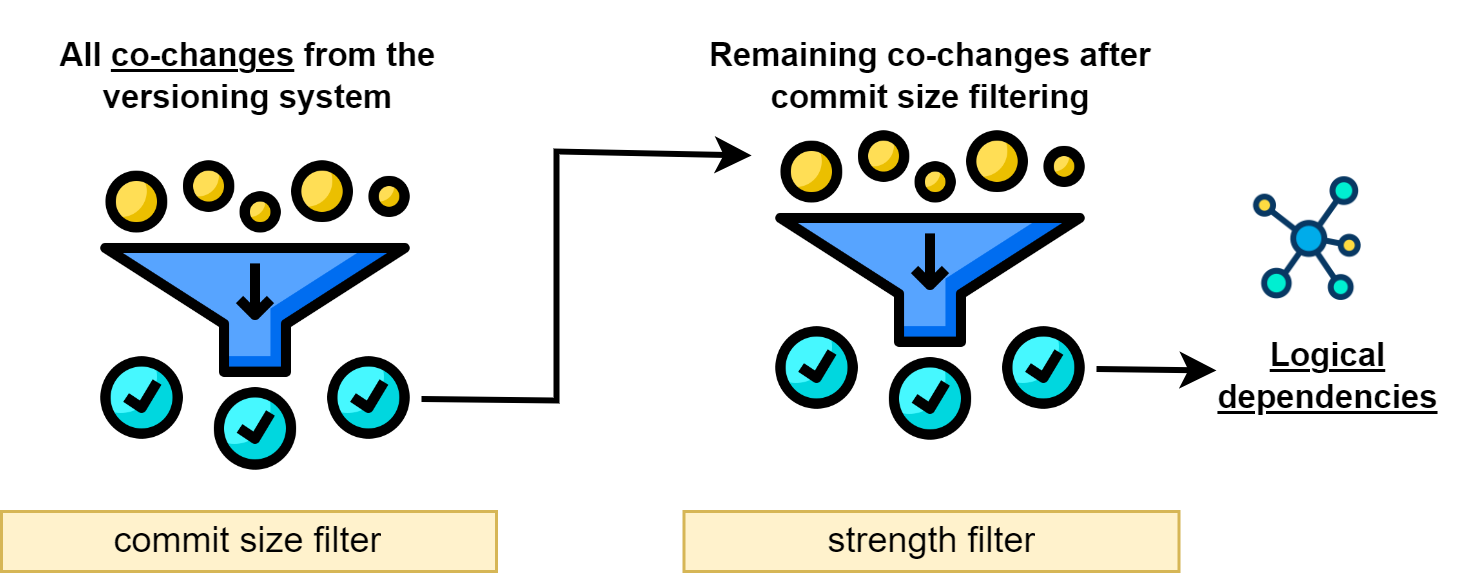
\includegraphics[width=\columnwidth]{filtering.png}
  \caption{Filter application process}
  \label{fig:filtering}
\end{figure}

\subsubsection{Dependency Extraction and Filtering Tool}

To extract and filter the co-changes, we used a previously developed tool \cite{b4}. This tool takes the GitHub repository address and the threshold values for commit and strength filters as input. The tool clones the repository, downloads all commit diffs starting from the first commit, examines all files changed in each commit to identify which entities have changed in those files, and creates undirected co-change dependencies between all changed entities within a commit.

The commit size filter is applied to these undirected co-change dependencies since the metric value for $(A \rightarrow B)$ is the same as for $(B \rightarrow A)$. For the strength filter, each co-change dependency is converted into a directed co-change dependency, so for each $(A \rightarrow B)$ dependency, we have both $(A \rightarrow B)$ and $(B \rightarrow A)$. This conversion is necessary because, as mentioned in the previous section, the confidence filter evaluates the rule's antecedent. Thus, the metric value for $(A \rightarrow B)$ differs from the metric value for $(B \rightarrow A)$.

After applying the filters, the remaining dependencies are exported to a CSV file for further use.

It is important to note that the strength metric is only used for filtering and is \textit{not considered as a weight} of the dependencies. The \textit{weight assigned to each dependency is the number of commits in which both entities were updated together}.


\subsubsection{Combining Structural and Logical Dependencies}


\begin{figure}[t!]
  \centering
  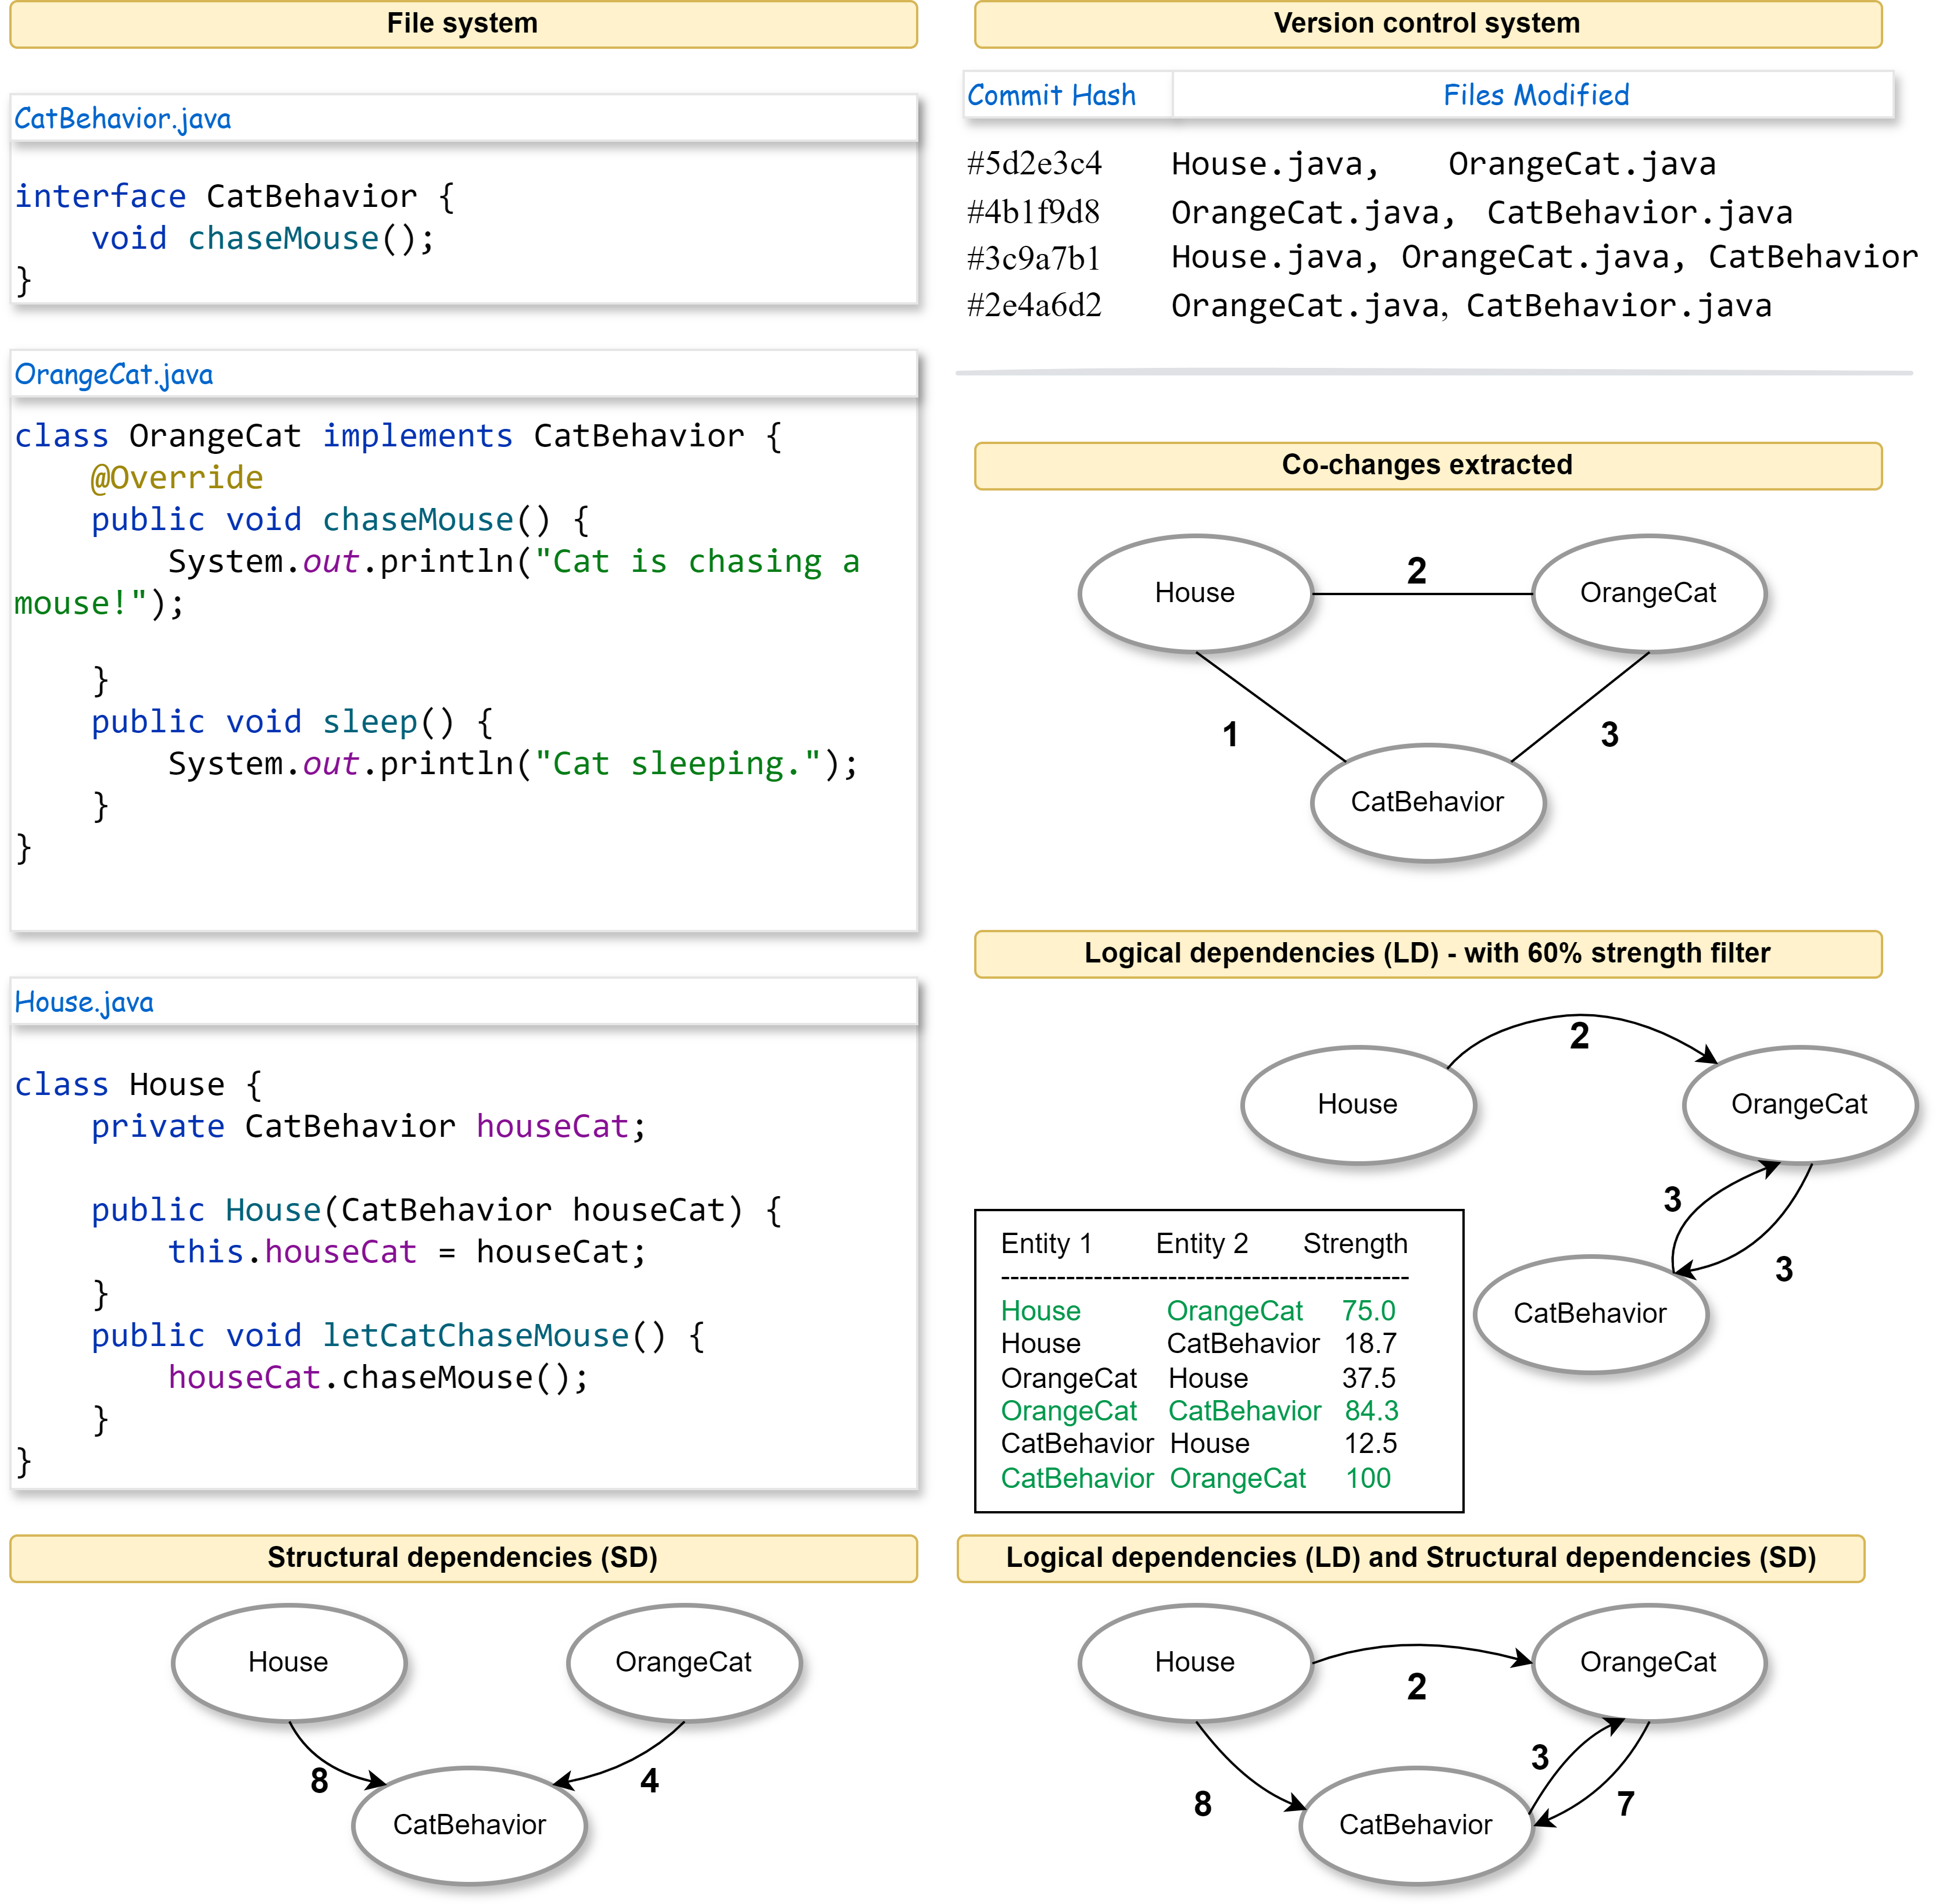
\includegraphics[width=\columnwidth]{codegraph.png}
  \caption{Dependency Graph: Combining structural and logical dependencies.}
  \label{fig:codegraph}
\end{figure}

When structural dependencies (SD) and logical dependencies (LD) are combined in software clustering, both types of relationships are represented within the same graph.

Each entity in the system is represented as a node in the graph, and the dependencies between them are represented as directed weighted edges.

\textit{SD and LD weights are combined} when the same pair of entities appear in both dependencies. In this case, the weights from SD and LD are summed, giving more influence to those entity pairs. When a pair of entities appear only in SD or only in LD, the edge is added to the graph together with its corresponding weight.

Figure \ref{fig:codegraph} illustrates combining structural and logical dependencies in the same dependency graph. The structural dependencies between \texttt{House}, \texttt{OrangeCat}, and \texttt{CatBehavior} entities are visible from the source code analysis.

However, the combination of SD and LD reveals additional insights. One important observation is the logical dependency between \texttt{House} and \texttt{OrangeCat}, which is not observed from the structural analysis. This relation is extracted from version control and filtered using a 60\% strength filter. The strength metric reveals that \texttt{House} and \texttt{OrangeCat} have a significant co-change value of 75.0, usually associated with a strong relationship.

When SD and LD overlap, such as between \texttt{OrangeCat} and \texttt{CatBehavior}, their weights are summed. This summation increases the weight of the dependency, making it more important in the dependency graph.



%%%%%%%%%%%%%%%%%%%%%%%%%%%%%%%%%%%%%%%%%%%%%%%%%%%%%


\section{Methodology and Implementation}
\label{sec:methodology_implementation}

In this section, we present the methodology used to evaluate the impact of logical dependencies on the quality of software clustering solutions.

First, we describe the clustering algorithms used in our experiments: Louvain, Leiden, and DBSCAN. Next, we introduce the evaluation metrics used to assess the quality of the clustering results. Finally, we present the workflow and implementation of the tool developed for this research, which is built to process structural and logical dependencies, apply the selected clustering algorithms, and compute the evaluation metrics.

\subsection{Clustering Algorithms}
\subsubsection{Louvain}
\label{subsubsec:louvain}

The Louvain algorithm was originally developed by Blondel et al. and is used to find community partitions (clusters) in large networks. The algorithm begins with a weighted network of N nodes, initially assigning each node to its own cluster, resulting in N clusters. For each node, the algorithm evaluates the modularity gained from moving the node to the cluster of each of its neighbors. Based on the results, the node is moved to the cluster with the maximum positive modularity gain. This process is repeated for all nodes until no further improvement in modularity is possible \cite{b8}, \cite{b9}.

\subsubsection{Leiden}
\label{subsubsec:leiden}

The Leiden algorithm, developed by Traag et al., is an improvement over the Louvain algorithm for community detection in large networks. Like Louvain, the Leiden algorithm begins with each node assigned to its own cluster and iteratively moves nodes between clusters to optimize modularity. However, the Leiden algorithm addresses some problems of the Louvain method, particularly regarding poorly connected communities and runtime performance issues \cite{leiden} \cite{scikit}.

The Leiden algorithm introduces a refinement phase that ensures communities are locally optimally clustered and well-connected. This refinement step distinguishes the Leiden algorithm from Louvain.


\subsubsection{DBSCAN}
\label{subsubsec:dbscan}

The Density-Based Spatial Clustering of Applications with Noise (DBSCAN) algorithm, introduced by Ester et al., is a density-based clustering algorithm for identifying clusters of arbitrary shape and detecting noise in data \cite{dbscan}, \cite{scikit}.

DBSCAN operates based on two main parameters:

\begin{itemize}
\item \textbf{Eps}: It defines the radius within which to search for neighboring points.
\item \textbf{MinPts}: The minimum number of points required for a dense region. It determines the minimum number of neighbors a point should have to be considered a core point.
\end{itemize}

The algorithm classifies points into three categories:

\begin{enumerate}
\item \textbf{Core Points}: Points that have at least \textit{MinPts} neighbors within a radius of \textit{Eps}. These points are located in the interior of a cluster.
\item \textbf{Border Points}: Points that have fewer than \textit{MinPts} neighbors within a radius of \textit{Eps} but are in the Eps-neighborhood of a core point. They are located on the edge of a cluster.
\item \textbf{Noise}: Points that are neither core points nor border points.
\end{enumerate}

The DBSCAN algorithm starts by visiting an arbitrary point in the dataset. If the point is a core point, the algorithm starts a new cluster and retrieves all reachable points from this core point. All points are then marked as part of the cluster. If the point is a border point, it moves to the next point in the dataset. This process is repeated until all points have been visited.

DBSCAN can be applied for software clustering by considering software entities as data points. A distance measure based on dependency weights can be used to compute the neighborhood between entities.

\subsection{Clustering Result Evaluation}
\label{subsec:evaluation_def}

We evaluate the clustering results using two metrics: the Modularity Quality (MQ) metric and the Move and Join Effectiveness Measure (MoJoFM) metric. Each provides a different perspective on the quality of the clustering solutions.

\subsubsection{Modularity Quality Metric}
\label{subsec:mq}

Mancoridis et al. introduced the Modularity Quality (MQ) metric to evaluate the modularization quality of a clustering solution based on the interaction between modules (clusters) \cite{b101},\cite{b10}. It evaluates the difference between connections within clusters and connections between different clusters.

The MQ of a graph partitioned into \( k \) clusters, where \( A_i \) is the Intra-Connectivity of the \( i \)-th cluster and \( E_{ij} \) is the Inter-Connectivity between the \( i \)-th and \( j \)-th clusters, is calculated using Equation \eqref{eq:mq} \cite{b2}.

\begin{equation}
MQ = \left( \frac{1}{k} \sum_{i=1}^{k} A_i \right) - \left( \frac{1}{k(k-1)} \sum_{i,j=1}^{k} E_{ij} \right)
\label{eq:mq}
\end{equation}

The MQ metric's value ranges between -1 and 1. A value of -1 means that the clusters have more connections between the clusters than within the clusters, while a value of 1 means that there are more connections within clusters than between clusters. A good clustering solution should have an MQ value close to 1, since this indicates that the clusters are more cohesive internally and have fewer connections to other clusters.

The MQ metric is useful because it does not require additional input besides the clustering result. It relies on the structure of the clustered entities and their interactions.

\subsubsection{MoJoFM Metric}
\label{subsec:mojofm}
Wen and Tzerpos introduced the MoJoFM metric to evaluate the similarity between two different software clustering results \cite{mojofm}. The metric is based on the MoJo metric, which measures the absolute minimum number of \textit{Move} and \textit{Join} operations required to transform one clustering solution into another \cite{b3}, \cite{mojofm}. However, MoJoFM provides a similarity measure ranging between 0\% and 100\%, where 100\% indicates identical clustering solutions.

The MoJoFM metric is calculated using Equation \eqref{eq:mojofm}:

\begin{equation}
\text{MoJoFM}(A, B) = \left(1 - \frac{\text{mno}(A, B)}{\max(\text{mno}(\forall A, B))}\right) \times 100\%
\label{eq:mojofm}
\end{equation}

Where:

\begin{itemize}
\item $\text{mno}(A, B)$ is the minimum number of \textit{Move} and \textit{Join} operations required to transform clustering solution $A$ into clustering solution $B$.
\item $\max(\text{mno}(\forall A, B))$ is the maximum possible number of such operations required to transform any clustering $A$ into clustering $B$.
\end{itemize}

To use the metric, we first need to generate a reference clustering solution for comparison. We manually created this reference based on our analysis of the codebase.

Using the MoJoFM metric, we can evaluate the similarity between the generated and reference clustering solutions. This metric is useful when combining multiple dependencies because it measures the similarity between the obtained clustering solutions and the same reference.


\subsection{Workflow for Software Clustering and Evaluation}
\label{subsec:tool_workflow}


\begin{figure}[t!]
  \centering
  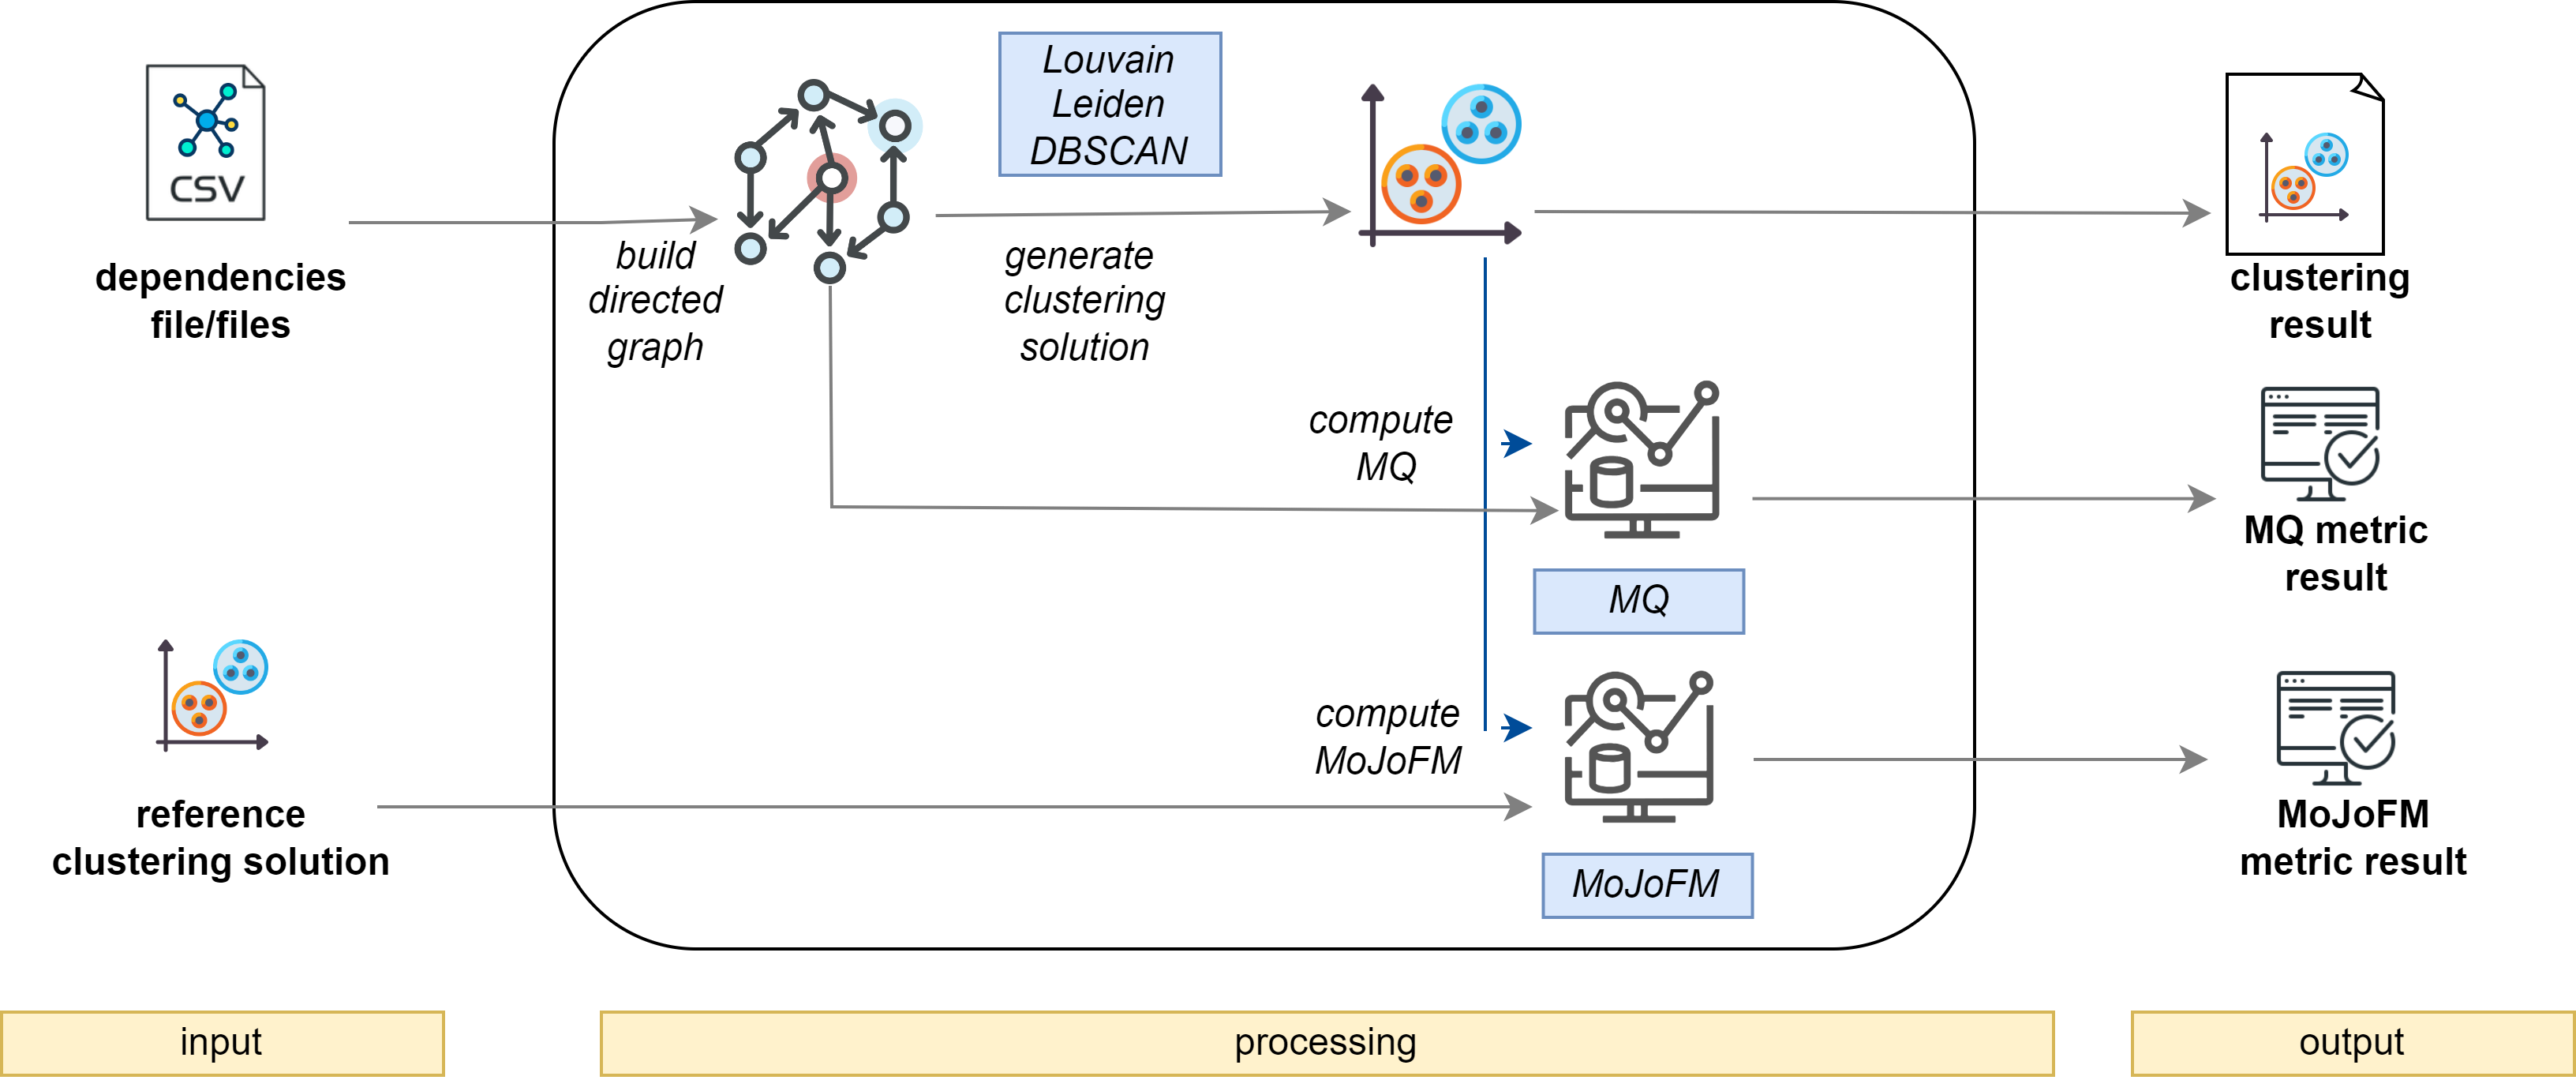
\includegraphics[width=\columnwidth]{workflow-tool.png}
  \caption{ \textbf{Tool workflow overview: input, processing and output.}}
  \label{fig:tool}
\end{figure}

To evaluate how logical dependencies impact the quality of clustering solutions, we developed a Python tool capable of using any type of dependency, either alone or combined with other types of dependencies, as long as it is provided in CSV format. The tool clusters and evaluates software clustering solutions using the MQ or MoJoFM metrics.



\subsubsection{Input}

The tool takes one or multiple dependency CSV files as input and the reference solution required for the MoJoFM metric. We designed the tool to accept multiple dependency files so that we can generate clustering solutions based on either a single type of dependency (structural or logical) or a combination of both.

Since the MoJoFM metric requires a reference solution to evaluate the obtained clustering solutions, we manually inspected the code and created reference clustering solutions, which we then provided as input for the tool.

\subsubsection{Processing}

The dependencies are saved in the CSV file in the following format: \texttt{antecedent of a dependency, consequent of a dependency, weight}. The tool reads each line, adds the antecedent and consequent as nodes in a directed graph, and creates an edge between them, with the weight from the CSV file becoming the edge weight. The edge weights are summed if multiple dependency files are processed and the same dependency is found in multiple files.

The workflow of applying the clustering algorithms and performing the evaluations is shown in Figure \ref{fig:tool}. After all dependencies are read, the directed graph is passed to the clustering algorithms: Louvain, Leiden, and DBSCAN. Each algorithm generates its own clustering result. The results from each algorithm are then evaluated using the MQ metric and the MoJoFM metric. The MQ metric requires the directed graph and the clustering result, while the MoJoFM metric requires the reference clustering solution provided as input and the clustering result.


\subsubsection{Output}

After applying each clustering algorithm and completing both evaluations, we export the clustering result, the number of clusters from the clustering solution, and the MQ and MoJoFM metrics values.


%%%%%%%%%%%%%%%%%%%%%%%%%%%%%%%%%%%%%%%%%%%%%%%%%%%%%%%%%%

\section{Experimental Plan and Results}
\label{sec:experiment}


\subsection{Experimental Plan}
\label{subsec:plan}

\subsubsection{Overview of projects used}

\begin{table}[!h]
\renewcommand{\arraystretch}{1}
\centering
\caption{Overview of projects used in experimental analysis}
\label{tab:project_info}
\scalebox{0.7}{
\begin{tabular}{|c|c|c|c|p{3cm}|}
\hline
\textbf{Project Name} & \textbf{Release Tag} & \textbf{Commits} & \textbf{GitHub Repository Link} & \textbf{Repository Description} \\ \hline
Apache Ant & 1.10.13 & 14,917 & https://github.com/apache/ant & Java build tool for automating software tasks. \\ \hline
Apache Tomcat & 8.5.93 & 22,698 & https://github.com/apache/tomcat & Java web server and servlet container. \\ \hline
Hibernate ORM & 6.2.14 & 16,609 & https://github.com/hibernate/hibernate-orm & Java ORM framework for database management. \\ \hline
Gson & gson-parent-2.10.1 & 1,772 & https://github.com/google/gson & Java library for JSON serialization and deserialization. \\ \hline
\end{tabular}
}
\end{table}

In Table \ref{tab:project_info}, we have synthesized all the information about the four projects used in our experiments. The 'Project Name' column contains the names of the software projects sourced from GitHub. The 'Release Tag' column contains the specific release tag of the project that was analyzed. We processed all the commits for logical dependency extraction, from the first commit to the commit associated with the specified tag. We extracted the dependencies from the code of that specific tag for structural dependencies. The 'Number of Commits' column provides the total number of commits used for logical dependencies extraction. The 'GitHub Repository Link' column includes the URL link to the project's repository on GitHub. Finally, the 'Repository Description' column briefly describes the project's purpose and functionality.

We mainly chose projects with more than 10,000 commits in their commit history so that the logical dependencies extraction can be done on a more extensive information base. However, we selected Gson, which has a relatively small commit history (1,772 commits), to determine if our experiments work with a smaller information base.

\subsubsection{Tool runs}

To assess the impact of logical dependencies and to answer the research questions from section \ref{sec:introduction}, we run the tool presented in Section \ref{subsec:tool_workflow} in three different scenarios for all the projects from table \ref{tab:project_info}. All three scenarios are illustrated in Fig. \ref{fig:scenatrio}.

In the first scenario, we run the tool once, providing only the system's structural dependencies as input for the clustering algorithm.

In the second scenario, we run the tool ten times, using only logical dependencies as input. We perform ten runs because we generate logical dependencies with different threshold values for the strength filter. We start with a threshold of 10 and increase it in steps of 10 up to 100, where 100 is the maximum value for the threshold.

In the third scenario, we combine logical with structural dependencies. Similar to the second scenario, we ran the tool ten times using structural and logical dependencies generated with different strength thresholds.

\begin{figure}[t!]
  \centering
  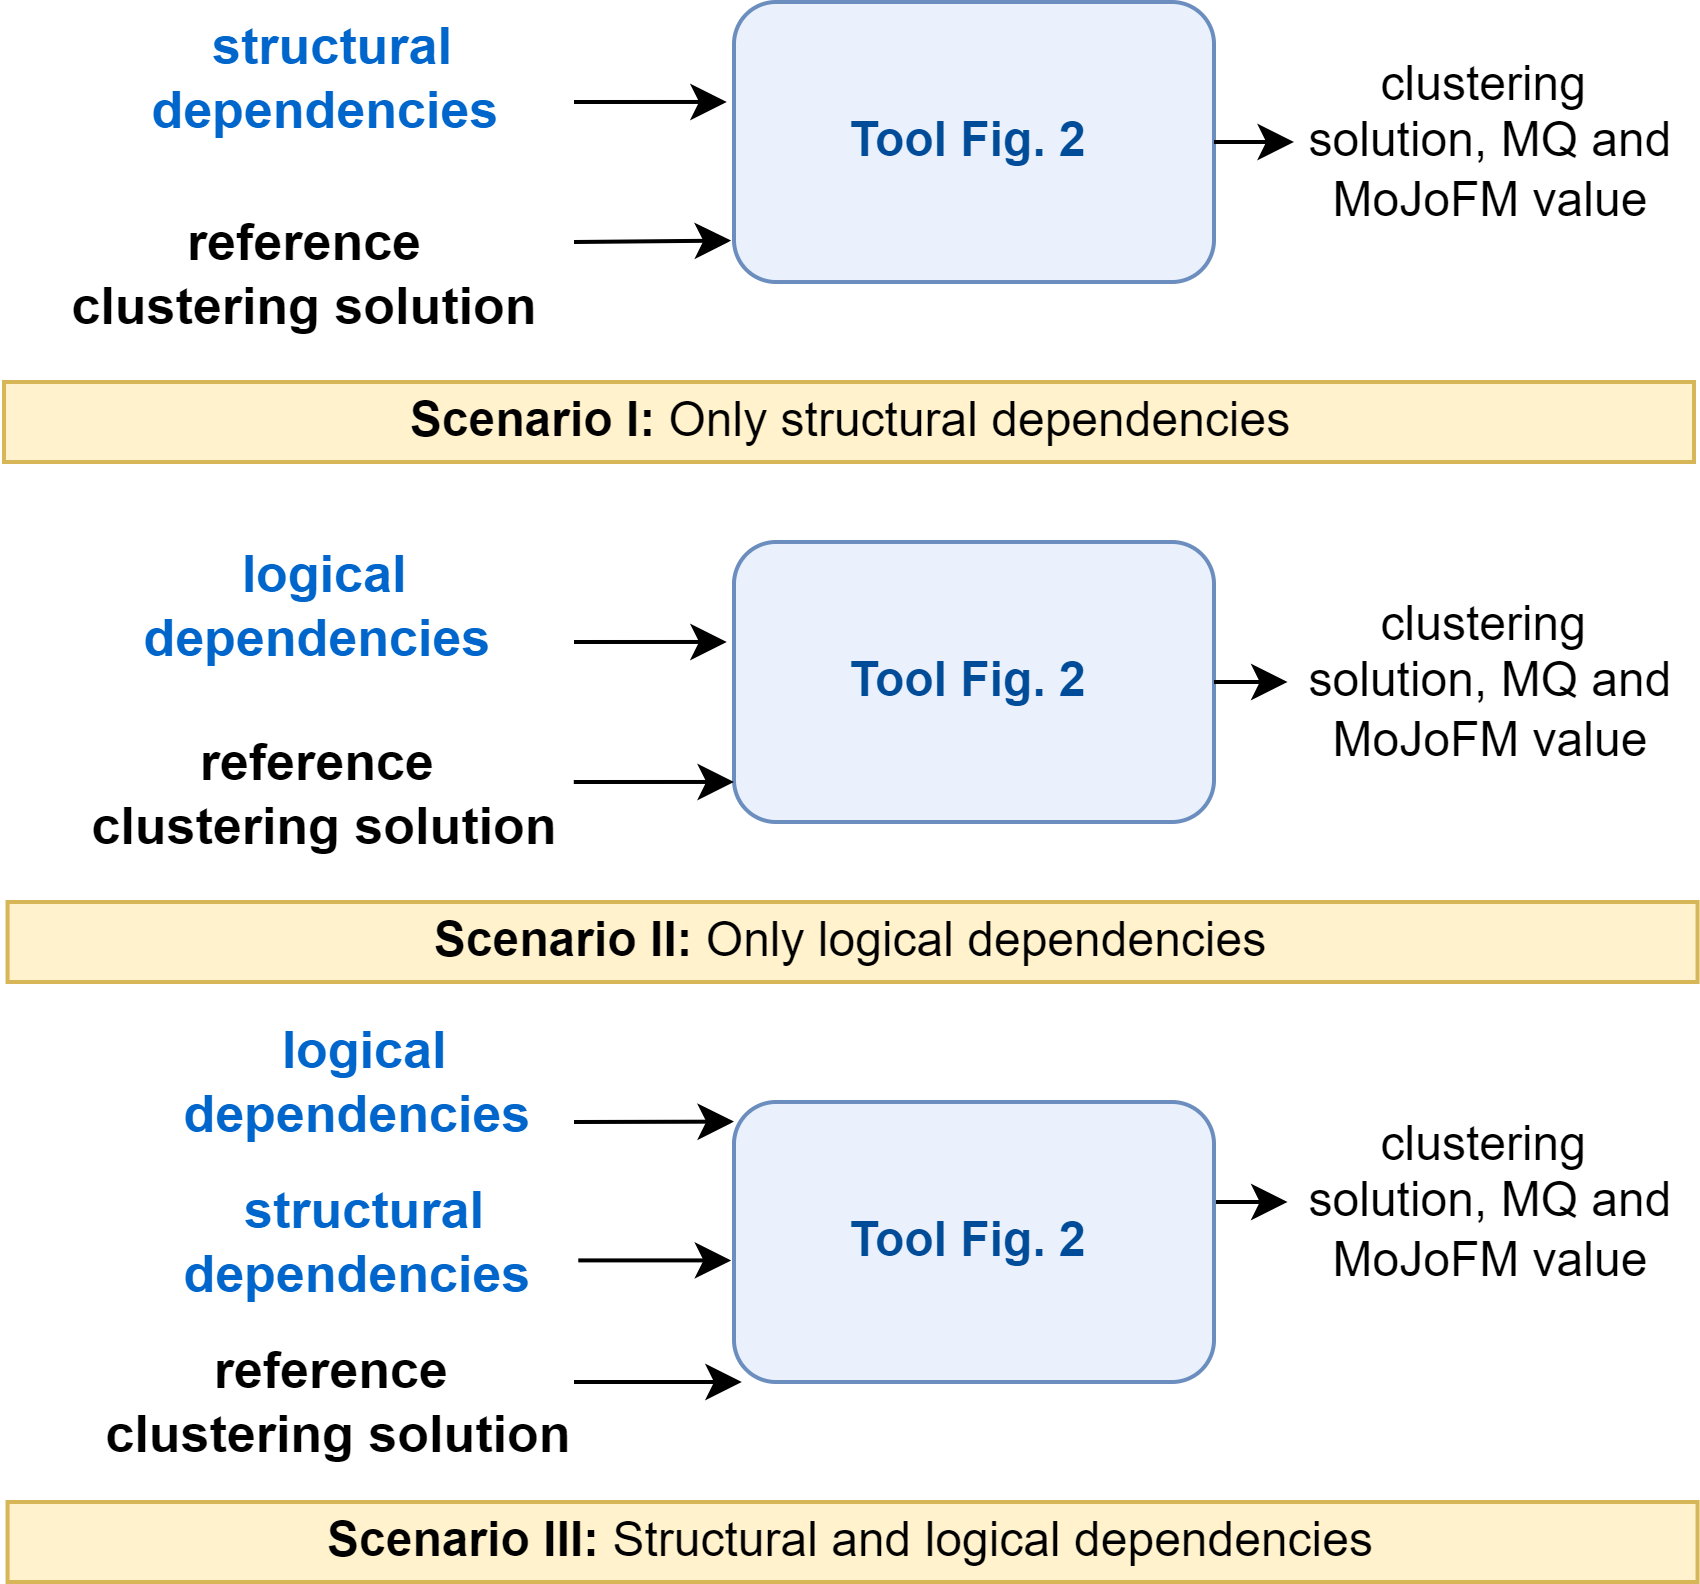
\includegraphics[width=\columnwidth]{scenario.png}
  \caption{ \textbf{Experimental scenarios for analyzing the impact of logical dependencies on clustering quality}}
  \label{fig:scenatrio}
\end{figure}

\subsection{Results}
\label{subsec:results}

The experimental results are presented in this subsection in four tables, each corresponding to a different project. Table \ref{tab:clustering_results_ant} presents the results for Apache Ant, Table \ref{tab:clustering_results_tomcat} presents the results for Apache Tomcat, Table \ref{tab:clustering_results_hibernate} presents the results for Hibernate ORM, and Table \ref{tab:clustering_results_gson} presents the results for Gson.

Each table includes the following columns:
\begin{itemize}
\item \textbf{Dependency Type:} The types of dependencies used are as follows: SD for Structural Dependencies, LD for Logical Dependencies, and SD+LD for their combination. The strength threshold used is specified in parentheses right after LD.
\item \textbf{Entities Count:} The total number of software entities (such as classes, interfaces, enums) involved in clustering.
\item \textbf{System Coverage:} Considering that the total number of entities extracted from the codebase — which represents the entities forming structural dependencies (SD) — constitutes the entire set of entities in the system (the first line of each table), we calculated the percentage of entities present in the filtered logical dependencies (LD) relative to the total number of known codebase entities.
\item \textbf{Louvain/ Leiden/ DBSCAN:} The clustering algorithms used in the experiments.
\item \textbf{Nr. of Clusters:} The number of clusters from the clustering solution.
\item \textbf{MQ (Modularization Quality):} The result obtained when applying the MQ evaluation metric to the clustering solution.
\item \textbf{MoJoFM:} The result obtained when applying the MoJoFM evaluation metric to the clustering solution.
\end{itemize}

The rows in each table represent different dependency types and strength filter thresholds used in the clustering experiments.



\begin{table}[htbp]
\centering
\caption{Clustering results based on different dependency types and strength filter thresholds for repository: https://github.com/apache/ant}
\label{tab:clustering_results_ant}
\resizebox{\textwidth}{!}{
\begin{tabular}{|l|c|c|ccc|ccc|ccc|}
\hline
 \textbf{Dependency} &  \textbf{Entities} & \textbf{System} & \multicolumn{3}{c|}{\textbf{Louvain}} & \multicolumn{3}{c|}{\textbf{Leiden}} & \multicolumn{3}{c|}{\textbf{DBSCAN}} \\
\cline{4-12}
\textbf{Type (strength } &  \textbf{Count} & \textbf{Coverage} & \textbf{Nr. of } & \textbf{MQ} & \textbf{MojoFM} & \textbf{Nr. of} & \textbf{MQ} & \textbf{MojoFM} & \textbf{Nr. of} & \textbf{MQ} & \textbf{MojoFM}  \\
\textbf{threshold)} &  & \textbf{(\%)} & \textbf{clusters} & & & \textbf{clusters} & &  & \textbf{clusters} & &\\
\hline
\rowcolor[HTML]{ECECEC} \textbf{SD} & 517 & 100.00 & 14 & 0.114 & 46.02 & 14 & 0.101 & 52.99 & 34 & 0.144 & 25.1  \\
\textbf{LD (10)} & 320 & 61.89 & 55 & 0.506 & 65.57 & 55 & 0.506 & 65.57 & 30 & 0.435 & 39.02 \\
\textbf{LD (20)} & 215 & 41.58 & 53 & 0.547 & 68 & 53 & 0.547 & 68 & 23 & 0.505 & 53.5 \\
\textbf{LD (30)} & 174 & 33.65 & 44 & 0.558 & 71.7 & 44 & 0.558 & 71.7 & 19 & 0.585 & 50 \\
\textbf{LD (40)} & 152 & 29.40 & 40 & 0.580 & 71.53 & 40 & 0.580 & 71.53 & 19 & 0.602 & 53.06 \\
\textbf{LD (50)} & 138 & 26.69 & 35 & 0.604 & 73.98 & 35 & 0.604 & 73.98 & 17 & 0.633 & 56.1 \\
\textbf{LD (60)} & 120 & 23.21 & 34 & 0.587 & 70.48 & 34 & 0.587 & 70.48 & 14 & 0.650 & 51.43 \\
\textbf{LD (70)} & 106 & 20.50 & 32 & 0.577 & 71.43 & 32 & 0.577 & 71.43 & 11 & 0.661 & 51.65 \\
\textbf{LD (80)} & 92 & 17.79 & 29 & 0.576 & 70.13 & 29 & 0.576 & 70.13 & 9 & \cellcolor[HTML]{FEF9E4}0.709 & 50.65 \\
\textbf{LD (90)} & 79 & 15.28 & 24 & 0.606 & 71.88 & 24 & 0.606 & 71.88 & 8 & 0.705 & 56.6 \\
\textbf{LD (100)} & 64 & 12.37 & 19 & \cellcolor[HTML]{fef9e4}0.611 & \cellcolor[HTML]{fef9e4}75.51 & 19 & \cellcolor[HTML]{fef9e4}0.611 & \cellcolor[HTML]{fef9e4}75.51 & 6 & 0.691 & \cellcolor[HTML]{fef9e4}56.93 \\
\hline
\textbf{SD+LD (10)} & 517 & 100.00 & 18 & \cellcolor[HTML]{fef9e4}0.355 & \cellcolor[HTML]{fef9e4}55.18 & 15 & 0.254 & \cellcolor[HTML]{fef9e4}54.98 & 37 & 0.147 & 25.9 \\
\textbf{SD+LD (20)} & 517 & 100.00 & 17 & 0.318 & 52.39 & 19 & \cellcolor[HTML]{fef9e4}0.365 & 53.78 & 32 & 0.149 & \cellcolor[HTML]{fef9e4}26.49 \\
\textbf{SD+LD (30)} & 517 & 100.00 & 16 & 0.282 & 53.19 & 16 & 0.265 & 54.78 & 30 & \cellcolor[HTML]{FEF9E4}0.159 & 24.5 \\
\textbf{SD+LD (40)} & 517 & 100.00 & 17 & 0.340 & 51.99 & 17 & 0.317 & 53.19 & 31 & 0.146 & 24.7 \\
\textbf{SD+LD (50)} & 517 & 100.00 & 15 & 0.248 & 52.59 & 19 & 0.298 & 56.77 & 31 & 0.146 & 24.7 \\
\textbf{SD+LD (60)} & 517 & 100.00 & 16 & 0.244 & 50.8 & 16 & 0.271 & 54.38 & 32 & 0.155 & 25.1 \\
\textbf{SD+LD (70)} & 517 & 100.00 & 15 & 0.238 & 51.00 & 18 & 0.281 & 52.99 & 32 & 0.155 & 25.1 \\
\textbf{SD+LD (80)} & 517 & 100.00 & 13 & 0.246 & 45.22 & 15 & 0.255 & 45.82 & 32 & 0.155 & 25.1 \\
\textbf{SD+LD (90)} & 517 & 100.00 & 14 & 0.258 & 46.02 & 16 & 0.268 & 47.01 & 32 & 0.155 & 25.1 \\
\textbf{SD+LD (100)} & 517 & 100.00 & 15 & 0.214 & 50.8 & 15 & 0.227 & 50.4 & 32 & 0.155 & 25.1 \\
\hline
\end{tabular}
}
\end{table}



\begin{table*}[htbp]
\centering
\caption{Clustering results based on different dependency types and strength filter thresholds for repository: https://github.com/apache/tomcat}
\label{tab:clustering_results_tomcat}
\resizebox{\textwidth}{!}{
\begin{tabular}{|l|c|c|ccc|ccc|ccc|}
\hline
 \textbf{Dependency} &  \textbf{Entities} & \textbf{System} & \multicolumn{3}{c|}{\textbf{Louvain}} & \multicolumn{3}{c|}{\textbf{Leiden}} & \multicolumn{3}{c|}{\textbf{DBSCAN}} \\
\cline{4-12}
\textbf{Type (strength } &  \textbf{Count} & \textbf{Coverage} & \textbf{Nr. of } & \textbf{MQ} & \textbf{MojoFM} & \textbf{Nr. of} & \textbf{MQ} & \textbf{MojoFM} & \textbf{Nr. of} & \textbf{MQ} & \textbf{MojoFM}  \\
\textbf{threshold)} &  & \textbf{(\%)} & \textbf{clusters} & & & \textbf{clusters} & &  & \textbf{clusters} & &\\
\hline
\rowcolor[HTML]{ECECEC} \textbf{SD} & 662 & 100.00 & 26 & 0.186 & 77.76 & 24 & 0.184 & 76.99 & 43 & 0.142 & 73.31  \\
\textbf{LD (10)} & 406 & 61.33 & 42 & 0.505 & 72.47 & 42 & 0.505 & 72.47 & 60 & 0.393 & 67.93 \\
\textbf{LD (20)} & 303 & 45.77 & 45 & 0.538 & 68.26 & 45 & 0.538 & 67.24 & 41 & 0.510 & 72.7 \\
\textbf{LD (30)} & 249 & 37.61 & 46 & 0.532 & 69.87 & 46 & 0.532 & 69.87 & 32 & 0.561 & 80.33 \\
\textbf{LD (40)} & 208 & 31.42 & 42 & 0.590 & 69.70 & 42 & 0.591 & 70.71 & 28 & 0.572 & 83.84 \\
\textbf{LD (50)} & 198 & 29.91 & 44 & 0.604 & 70.21 & 44 & 0.604 & 70.21 & 22 & 0.631 & 85.11 \\
\textbf{LD (60)} & 177 & 26.74 & 45 & 0.601 & 70.66 & 45 & 0.601 & 70.66 & 18 & 0.662 & 85.63 \\
\textbf{LD (70)} & 164 & 24.77 & 45 & 0.598 & 75.32 & 45 & 0.598 & 75.32 & 17 & 0.676 & 88.96 \\
\textbf{LD (80)} & 127 & 19.18 & 36 & 0.618 & 79.49 & 36 & 0.618 & 79.49 & 15 & 0.713 & \cellcolor[HTML]{fef9e4}89.74 \\
\textbf{LD (90)} & 116 & 17.52 & 32 & 0.623 & 81.13 & 32 & 0.623 & 81.13 & 14 & 0.718 & 89.62 \\
\textbf{LD (100)} & 110 & 16.62 & 30 & \cellcolor[HTML]{fef9e4}0.640 & \cellcolor[HTML]{fef9e4}85.00 & 30 & \cellcolor[HTML]{fef9e4}0.640 & \cellcolor[HTML]{fef9e4}85.00 & 13 & \cellcolor[HTML]{fef9e4}0.735 & 89.00 \\
\hline
\textbf{SD+LD(10)} & 662 & 100.00 & 28 & \cellcolor[HTML]{fef9e4}0.324 & 78.99 & 28 & 0.324 & 78.99 & 40 & 0.161 & \cellcolor[HTML]{fef9e4}74.23 \\
\textbf{SD+LD(20)} & 662 & 100.00 & 31 & 0.287 & 78.22 & 30 & 0.320 & \cellcolor[HTML]{fef9e4}80.06 & 50 & 0.189 & 73.31 \\
\textbf{SD+LD(30)} & 662 & 100.00 & 32 & 0.296 & \cellcolor[HTML]{fef9e4}79.92 & 32 & 0.277 & 75.77 & 45 & \cellcolor[HTML]{fef9e4}0.209 & 73.47 \\
\textbf{SD+LD(40)} & 662 & 100.00 & 34 & 0.292 & 79.91 & 32 & \cellcolor[HTML]{fef9e4}0.326 & 78.22 & 43 & 0.198 & 73.47 \\
\textbf{SD+LD(50)} & 662 & 100.00 & 33 & 0.294 & 76.53 & 35 & 0.301 & 76.23 & 43 & 0.196 & 73.31 \\
\textbf{SD+LD(60)} & 662 & 100.00 & 35 & 0.304 & 77.15 & 33 & 0.286 & 76.84 & 41 & 0.177 & 73.62 \\
\textbf{SD+LD(70)} & 662 & 100.00 & 34 & 0.282 & 76.69 & 34 & 0.292 & 77.45 & 41 & 0.166 & 73.62 \\
\textbf{SD+LD(80)} & 662 & 100.00 & 34 & 0.283 & 76.23 & 33 & 0.282 & 76.38 & 42 & 0.153 & 73.47 \\
\textbf{SD+LD(90)} & 662 & 100.00 & 31 & 0.311 & 78.99 & 31 & 0.311 & 78.99 & 43 & 0.153 & 73.31 \\
\textbf{SD+LD(100)} & 662 & 100.00 & 31 & 0.311 & 78.83 & 31 & 0.305 & 78.37 & 43 & 0.153 & 73.31 \\
\hline
\end{tabular}
}
\end{table*}




\begin{table*}[htbp]
\centering
\caption{Clustering results based on different dependency types and strength filter thresholds for repository: https://github.com/hibernate/hibernate-orm}{https://github.com/hibernate/hibernate-orm}
\label{tab:clustering_results_hibernate}
\resizebox{\textwidth}{!}{
\begin{tabular}{|l|c|c|ccc|ccc|ccc|}
\hline
 \textbf{Dependency} &  \textbf{Entities} & \textbf{System} & \multicolumn{3}{c|}{\textbf{Louvain}} & \multicolumn{3}{c|}{\textbf{Leiden}} & \multicolumn{3}{c|}{\textbf{DBSCAN}} \\
\cline{4-12}
\textbf{Type (strength } &  \textbf{Count} & \textbf{Coverage} & \textbf{Nr. of } & \textbf{MQ} & \textbf{MojoFM} & \textbf{Nr. of} & \textbf{MQ} & \textbf{MojoFM} & \textbf{Nr. of} & \textbf{MQ} & \textbf{MojoFM}  \\
\textbf{threshold)} &  & \textbf{(\%)} & \textbf{clusters} & & & \textbf{clusters} & &  & \textbf{clusters} & &\\
\hline
\rowcolor[HTML]{ECECEC} \textbf{SD} & 4414 & 100.00 & 30 & 0.09 & 52.23 & 23 & 0.071 & 52.44 & 373 & 0.128 & 46.32  \\
\textbf{LD (10)} & 1450 & 32.85 & 44 & 0.389 & 57.22 & 45 & 0.39 & 58.22 & 99 & 0.395 & 57.08 \\
\textbf{LD (20)} & 1325 & 30.02 & 66 & 0.397 & 62.66 & 66 & 0.397 & 62.66 & 151 & 0.378 & 63.36 \\
\textbf{LD (30)} & 1222 & 27.68 & 66 & 0.38 & 62.45 & 67 & 0.38 & 63.04 & 148 & 0.378 & 65.42 \\
\textbf{LD (40)} & 915 & 20.73 & 84 & 0.417 & 63.68 & 85 & 0.412 & 63.56 & 110 & 0.382 & 66.9 \\
\textbf{LD (50)} & 900 & 20.39 & 84 & 0.409 & 64.56 & 84 & 0.409 & 64.56 & 105 & 0.386 & 67.02 \\
\textbf{LD (60)} & 848 & 19.21 & 82 & 0.406 & 63.26 & 81 & 0.41 & 63.39 & 104 & 0.379 & 65.13 \\
\textbf{LD (70)} & 459 & 10.40 & 89 & 0.516 & \cellcolor[HTML]{fef9e4}69.08 & 89 & 0.516 & \cellcolor[HTML]{fef9e4}69.08 & 41 & 0.467 & 58.21 \\
\textbf{LD (80)} & 450 & 10.19 & 91 & 0.506 & 68.64 & 91 & 0.506 & 68.64 & 39 & 0.479 & \cellcolor[HTML]{fef9e4}60.49 \\
\textbf{LD (90)} & 432 & 9.79 & 92 & 0.492 & 66.93 & 92 & 0.492 & 66.93 & 40 & 0.473 & 58.66 \\
\textbf{LD (100)} & 356 & 8.07 & 81 & \cellcolor[HTML]{fef9e4}0.524 & 65.92 & 81 & \cellcolor[HTML]{fef9e4}0.524 & 65.92 & 29 & \cellcolor[HTML]{fef9e4}0.537 & 58.2 \\
\hline
\textbf{SD+LD (10)} & 4414 & 100.00 & 19 & 0.096 & 53.93 & 19 & 0.099 & 52.28 & 282 & 0.121 & 46.01 \\
\textbf{SD+LD (20)} & 4414 & 100.00 & 21 & 0.126 & 52.85 & 23 & 0.122 & 56.21 & 309 & \cellcolor[HTML]{fef9e4}0.135 & 47.4 \\
\textbf{SD+LD (30)} & 4414 & 100.00 & 26 & 0.121 & 55.76 & 26 & 0.15 & 54.54 & 317 & 0.135 & \cellcolor[HTML]{fef9e4}49.45 \\
\textbf{SD+LD (40)} & 4414 & 100.00 & 27 & \cellcolor[HTML]{fef9e4}0.182 & \cellcolor[HTML]{fef9e4}54.57 & 28 & \cellcolor[HTML]{fef9e4}0.163 & \cellcolor[HTML]{fef9e4}55.89 & 350 & 0.134 & 49.35 \\
\textbf{SD+LD (50)} & 4414 & 100.00 & 26 & 0.16 & 52.37 & 24 & 0.147 & 53.31 & 350 & 0.134 & 49.37 \\
\textbf{SD+LD (60)} & 4414 & 100.00 & 26 & 0.161 & 52.35 & 27 & 0.153 & 53.19 & 352 & 0.135 & 49.31 \\
\textbf{SD+LD (70)} & 4414 & 100.00 & 28 & 0.139 & 52.78 & 29 & 0.154 & 54.34 & 366 & 0.13 & 47.13 \\
\textbf{SD+LD (80)} & 4414 & 100.00 & 28 & 0.142 & 52.83 & 28 & 0.147 & 53.35 & 366 & 0.13 & 47.72 \\
\textbf{SD+LD (90)} & 4414 & 100.00 & 28 & 0.136 & 52.62 & 30 & 0.153 & 53.83 & 365 & 0.13 & 47.72 \\
\textbf{SD+LD (100)} & 4414 & 100.00 & 30 & 0.128 & 52.78 & 28 & 0.114 & 55.23 & 365 & 0.128 & 47.75 \\
\hline
\end{tabular}
}
\end{table*}






\begin{table*}[htbp]
\centering
\caption{Clustering results based on different dependency types and strength filter thresholds for repository: https://github.com/google/gson}{https://github.com/google/gson}
\label{tab:clustering_results_gson}
\resizebox{\textwidth}{!}{
\begin{tabular}{|l|c|c|ccc|ccc|ccc|}
\hline
 \textbf{Dependency} &  \textbf{Entities} & \textbf{System} & \multicolumn{3}{c|}{\textbf{Louvain}} & \multicolumn{3}{c|}{\textbf{Leiden}} & \multicolumn{3}{c|}{\textbf{DBSCAN}} \\
\cline{4-12}
\textbf{Type (strength } &  \textbf{Count} & \textbf{Cover} & \textbf{Nr. of } & \textbf{MQ} & \textbf{MojoFM} & \textbf{Nr. of} & \textbf{MQ} & \textbf{MojoFM} & \textbf{Nr. of} & \textbf{MQ} & \textbf{MojoFM}  \\
\textbf{threshold)} &  & \textbf{(\%)} & \textbf{clusters} & & & \textbf{clusters} & &  & \textbf{clusters} & &\\
\hline
\rowcolor[HTML]{ECECEC} \textbf{gson SD} & 210 & 100.00 & 10 & 0.139 & 53.47 & 9 & 0.129 & 55.94 & 23 & 0.127 & 51.88 \\
\textbf{gson LD (10)} & 66 & 31.43 & 10 & 0.565 & 62.07 & 9 & 0.572 & 60.34 & 19 & 0.399 & 68.97 \\
\textbf{gson LD (20)} & 50 & 23.81 & 11 & 0.547 & 64.29 & 11 & 0.547 & 64.29 & 9 & 0.523 & 59.52 \\
\textbf{gson LD (30)} & 41 & 19.52 & 12 & 0.544 & 63.64 & 12 & 0.544 & 63.64 & 6 & 0.606 & 66.67 \\
\textbf{gson LD (40)} & 31 & 14.76 & 8 & \cellcolor[HTML]{fef9e4}0.635 & \cellcolor[HTML]{fef9e4}69.57 & 8 & \cellcolor[HTML]{fef9e4}0.635 & \cellcolor[HTML]{fef9e4}69.57 & 6 & \cellcolor[HTML]{fef9e4}0.612 & \cellcolor[HTML]{fef9e4}69.57 \\
\textbf{gson LD (50)} & 31 & 14.76 & 8 & 0.600 & 69.57 & 8 & 0.600 & 69.57 & 6 & 0.565 & 60.87 \\
\textbf{gson LD (60)} & 28 & 13.33 & 8 & 0.552 & 65.00 & 8 & 0.552 & 65.00 & 5 & 0.584 & 60.00 \\
\textbf{gson LD (70)} & 26 & 12.38 & 7 & 0.579 & 66.67 & 7 & 0.579 & 66.67 & 5 & 0.586 & 55.56 \\
\textbf{gson LD (80)} & 18 & 8.57 & 5 & 0.590 & 60.00 & 5 & 0.590 & 60.00 & 4 & 0.544 & 40.00 \\
\textbf{gson LD (90)} & 18 & 8.57 & 5 & 0.590 & 60.00 & 5 & 0.590 & 60.00 & 4 & 0.544 & 40.00 \\
\textbf{gson LD (100)} & 18 & 8.57 & 5 & 0.590 & 60.00 & 5 & 0.590 & 60.00 & 4 & 0.544 & 40.00 \\
\hline
\textbf{gson SD+LD(10)} & 210 & 100.00 & 11 & \cellcolor[HTML]{fef9e4}0.317 & \cellcolor[HTML]{fef9e4}64.36 & 11 & \cellcolor[HTML]{fef9e4}0.317 & \cellcolor[HTML]{fef9e4}64.36 & 20 & \cellcolor[HTML]{fef9e4}0.172 & \cellcolor[HTML]{fef9e4}63.86 \\
\textbf{gson SD+LD(20)} & 210 & 100.00 & 11 & 0.259 & 61.39 & 11 & 0.259 & 61.39 & 17 & 0.136 & 53.96 \\
\textbf{gson SD+LD(30)} & 210 & 100.00 & 11 & 0.277 & 61.39 & 11 & 0.277 & 61.39 & 20 & 0.136 & 55.94 \\
\textbf{gson SD+LD(40)} & 210 & 100.00 & 10 & 0.277 & 61.39 & 10 & 0.277 & 61.39 & 20 & 0.135 & 55.94 \\
\textbf{gson SD+LD(50)} & 210 & 100.00 & 10 & 0.270 & 60.40 & 11 & 0.270 & 60.89 & 20 & 0.135 & 55.94 \\
\textbf{gson SD+LD(60)} & 210 & 100.00 & 9 & 0.296 & 61.39 & 10 & 0.290 & 61.88 & 20 & 0.135 & 55.94 \\
\textbf{gson SD+LD(70)} & 210 & 100.00 & 8 & 0.295 & 59.41 & 8 & 0.295 & 59.41 & 20 & 0.135 & 55.94 \\
\textbf{gson SD+LD(80)} & 210 & 100.00 & 7 & 0.267 & 58.91 & 8 & 0.263 & 59.41 & 21 & 0.134 & 55.45 \\
\textbf{gson SD+LD(90)} & 210 & 100.00 & 7 & 0.267 & 58.91 & 7 & 0.267 & 58.91 & 21 & 0.134 & 55.45 \\
\textbf{gson SD+LD(100)} & 210 & 100.00 & 7 & 0.267 & 58.91 & 8 & 0.263 & 59.41 & 21 & 0.134 & 55.45 \\
\hline
\end{tabular}
}
\end{table*}


\begin{table}[htbp]
\centering
\begin{tabular}{|c|c|c|c|c|}
\hline
\textbf{Dependency type} & \textbf{Ant} & \textbf{Tomcat} & \textbf{Hibernate} & \textbf{Gson} \\ \hline
\rowcolor[HTML]{ECECEC}\textbf{SD}     & 5.91  & 6.91  & 5.41  & 5.24  \\
\textbf{LD(10)} & 11.17 & 12.82 & 2.45  & 14.15 \\
\textbf{LD(20)} & 16.01 & 19.65 & 3.00  & 19.10 \\ 
\textbf{LD(30)} & 18.08 & 23.56 & 3.27  & 27.58 \\ 
\textbf{LD(40)} & 19.08 & 25.57 & 4.63  & 29.85 \\ 
\textbf{LD(50)} & 19.94 & 26.31 & 4.80  & 29.97 \\ 
\textbf{LD(60)} & 24.26 & 28.91 & 5.14  & 33.93 \\ 
\textbf{LD(70)} & 26.70 & 30.35 & 9.53  & 34.37 \\ 
\textbf{LD(80)} & 30.83 & 35.33 & 10.18 & 43.00 \\ 
\textbf{LD(90)} & 32.11 & 36.90 & 10.47 & 43.00 \\ 
\textbf{LD(100)} & 33.93 & 37.04 & 12.00 & 43.00 \\
 \hline
\end{tabular}
\caption{Average weights of Structural Dependencies (SD) and Logical Dependencies (LD).}
\label{tab:systems_weights}
\end{table}


To better understand the impact of different dependency types on software clustering, we also analyzed the average weights assigned to structural dependencies (SD) and logical dependencies (LD) across the studied projects. Table \ref{tab:systems_weights} presents these average dependency weights. The first row shows the average weights for SD, which remain constant across all strength thresholds, while the other rows show the average weights for logical dependencies at different strength thresholds.



\section{Evaluation}
\label{sec:evaluation}

The overall analysis of all the results from subsection \ref{subsec:results} indicates that combining structural and logical dependencies (SD+LD) provides better clustering solutions than using structural dependencies (SD) alone, covering 100\% of the system, meaning that no entity is missed during cluster generation. On the other hand, logical dependencies (LD) alone result in better clustering quality metrics compared to both SD and SD+LD, but they do not cover the entire system.

The best results for SD+LD are observed with a strength threshold between 10-40\%. For LD only, the best results are obtained at a 100\% strength threshold. The overall trend shows that for LD only, the MQ metric increases in value with a higher strength threshold, indicating more cohesive clusters, while the MoJo metric decreases, indicating that fewer transformations are needed to reach the expected clustering. For SD+LD, the best MQ and MoJo values are obtained at lower strength thresholds, and then both metrics indicate a less effective clustering solution obtained with higher strength thresholds.

We analyze each project in detail in the sections below and address the research questions.

\subsection{Detailed results}

\subsubsection{Apache Ant}

The clustering results for Apache Ant (Table \ref{tab:clustering_results_ant}) show that the combined structural and logical dependencies (SD+LD) achieved the best values with a strength threshold between 10\% and 30\%. The highest value for the MQ metric is reached with Leiden at a strength threshold of 20\%, and the highest value for MoJoFM is also reached with Leiden at a strength threshold of 10\%.

Compared with the SD-only results, all SD+LD clustering solutions for all algorithms show better MQ metric values, with the highest MQ value for SD+LD being more than three times greater than the corresponding SD-only value. Similarly, the MoJoFM metric shows better results than SD-only. However, it does not always outperform the MoJoFM metric applied to SD-only data.

Logical dependencies (LD) alone produced the highest MQ and MoJoFM values at the 100\% strength threshold for both Leiden and Louvain, with the obtained metric values being higher than those of SD-only and SD+LD. However, the percentage of entities covered is significantly lower (LD(100) covers only 12.37\% of the system).
If we look at LD(10), where there is a 61.89\% coverage of the system, which is more compared to LD(100), both metrics still perform better than SD-only and SD+LD(10). However, there is still a gap until 100\% coverage.

From the clustering algorithm performance point of view, Leiden obtains the best evaluation metrics for all scenarios, followed by Louvain and DBSCAN.

One interesting observation is that, based on the LD-only results, where the metrics results improved with higher strength thresholds, the SD+LD results did not follow the same pattern. On the opposite, the SD+LD metric results decline with a higher strength threshold. An explanation for this behavior may lie in the overlap between structural and logical dependencies. As presented in Figure \ref{fig:ant_correlation}, the number of LD decreases with a stricter strength threshold compared to the number of SD, and the overlap between the two types of dependencies increases.

\begin{figure}[t!]
\centering
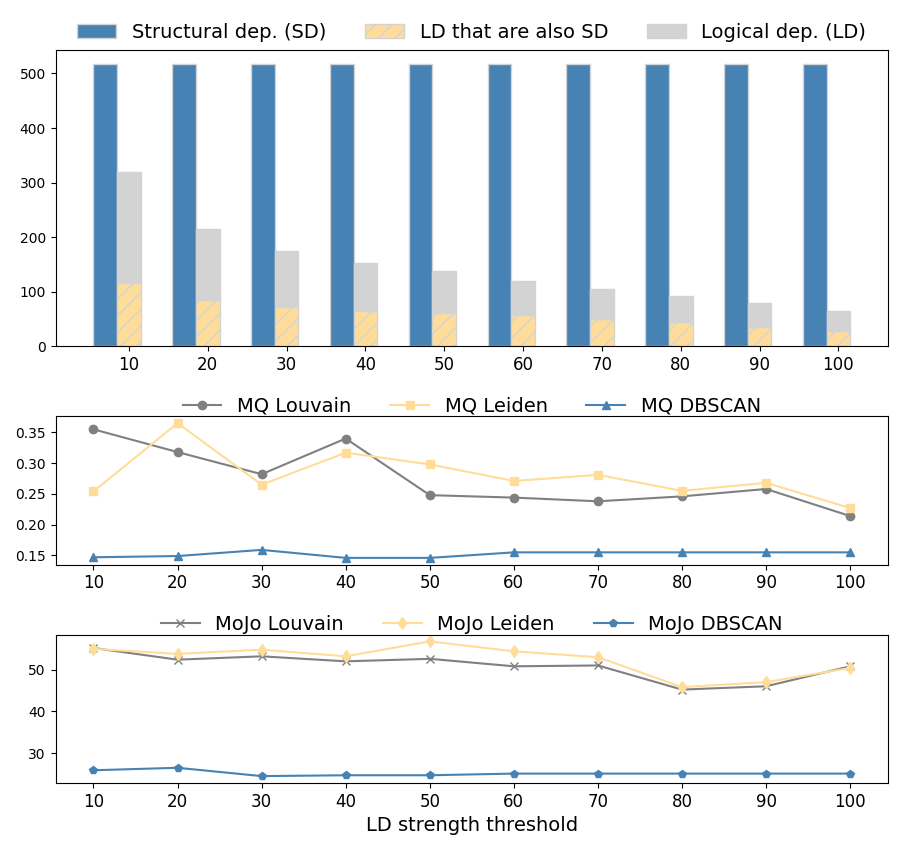
\includegraphics[width=\columnwidth]{ant_correlation.png}
\caption{\textbf{Apache Ant: Overlap between structural and logical dependencies and its correlation with clustering metrics.}}
\label{fig:ant_correlation}
\end{figure}

In our previous works, we studied how these two types of dependencies overlap \cite{b4}, \cite{b5}. The reason behind those studies was to check how much new information we can get from using logical dependencies and how much is already present via structural dependencies.

Our overall findings were that with stricter filtering of logical dependencies, we obtain a higher percentage of overlap between the two dependencies, reaching at most 50\% of logical dependencies that are also structural dependencies.

So, we consider that the reason why SD+LD clustering solutions decline in performance with a higher strength threshold is that less and less new additional information is added to the system (logical dependencies that are not structural dependencies), causing the clustering solution to start resembling the performance of the SD-only solution. In Figure \ref{fig:ant_correlation}, we can see that LD(10) represents 61\% of the quantity of SD, while LD(100) is only at 12\%, with half of them being duplicated with SD.

\subsubsection{Apache Tomcat}

For Apache Tomcat (Table \ref{tab:clustering_results_tomcat}), the best results for SD+LD were obtained with strength thresholds between 10\% and 40\% across all algorithms. The Leiden algorithm achieved the best result for the MQ metric at a strength threshold of 40\%, while the best MoJoFM result was obtained at a threshold of 20\%, also with the Leiden algorithm. Compared with the SD-only results, the peak MQ values almost double the SD-only values. Like Apache Ant, the MQ values for all strength thresholds are higher than those for SD-only. While MoJoFM is not better for all thresholds, it still improves compared with the SD-only results.

The LD-only results show the highest MQ and MoJoFM values at LD(100) for the Louvain and Leiden algorithms. However, as with the Apache Ant results, coverage remains an issue. LD(100) covers only 16.62\% of the system, lower than the coverage from SD-only or SD+LD combinations. On the other hand, LD(10), which covers 61.33\% of the system, still has better clustering solutions compared to SD-only, based on both MQ and MoJoFM results.

We observe the same decline in results with a stricter strength threshold for SD+LD. As with the previous system, these results can again be connected to the percentage of LD that also overlaps with SD and the decreasing number of LD compared to SD once the strength threshold becomes stricter. As shown in Figure \ref{fig:catalina_correlation}, LD filtered with a 10\% strength threshold overlaps with SD by approximately 22\%, while at a 100\% strength threshold, the overlap increases to approximately 39\%.

\begin{figure}[t!]
\centering
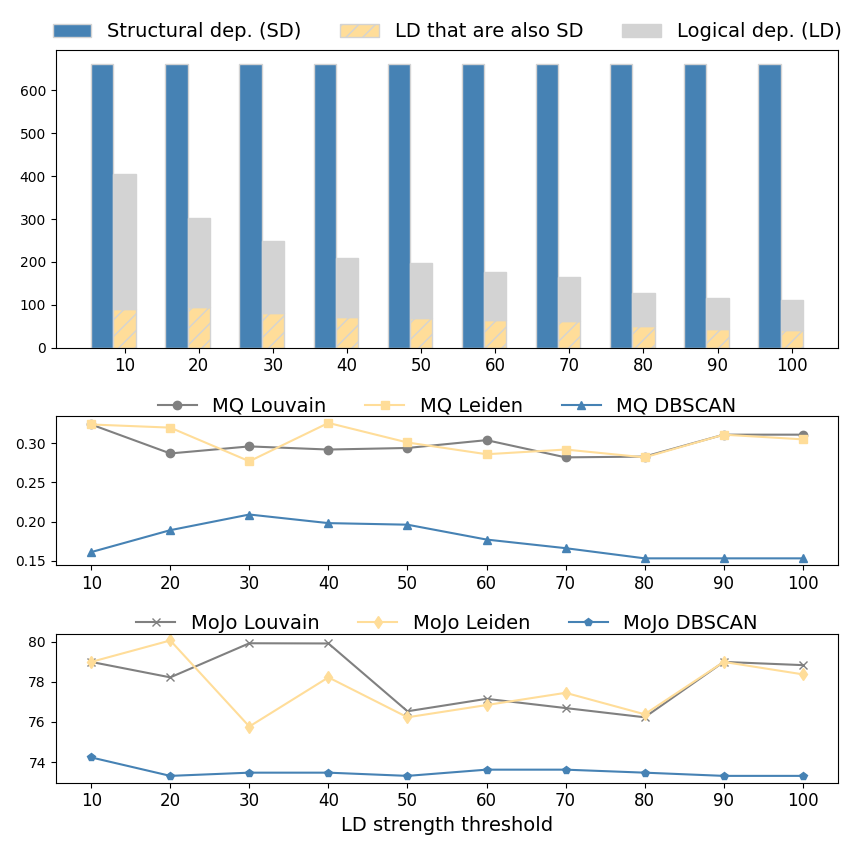
\includegraphics[width=\columnwidth]{catalina_correlation.png}
\caption{Apache Tomcat: Overlap between structural and logical dependencies and its correlation with clustering metrics.}
\label{fig:catalina_correlation}
\end{figure}

To ensure that the decline in performance for SD+LD with a stricter strength threshold is indeed caused by the fact that LD are significantly fewer than SD, and SD duplicates that part of them at higher thresholds, we added an additional experiment to our study. In this experiment, whose results can be found in Table \ref{tab:clustering_results_multiplication}, we increased the weights associated with LD(100) for Apache Tomcat to confirm that we are dealing with an LD quantity problem rather than a weight problem.

Therefore, in this experiment, we increased the weight assigned to each logical dependency filtered with a 100\% strength threshold from the Apache Tomcat system by values ranging from 1 to 5 and re-ran scenario III from Fig. \ref{fig:scenatrio}.


To maintain consistency, we used the same columns as in the other result tables (\ref{tab:clustering_results_ant}, \ref{tab:clustering_results_tomcat}, \ref{tab:clustering_results_hibernate}, \ref{tab:clustering_results_gson}), with the addition of two new columns:
\begin{itemize}
\item \textbf{Multiplication Factor:} The value by which each logical dependency weight is multiplied.
\item \textbf{Avg Weight:} The average weight assigned to each type of dependency used.
\end{itemize}

\begin{table}[htbp]
\centering
\caption{Impact of multiplication factors on clustering results for LD(100) in Apache Tomcat}
\label{tab:clustering_results_multiplication}
\resizebox{\textwidth}{!}{
\begin{tabular}{|l|c|c|ccc|ccc|ccc|}
\hline
\textbf{Multiplication} & \multicolumn{2}{c|}{\textbf{Avg. weight}} & \multicolumn{3}{c|}{\textbf{Louvain}} & \multicolumn{3}{c|}{\textbf{Leiden}} & \multicolumn{3}{c|}{\textbf{DBSCAN}} \\
\cline{4-12}
\textbf{Factor} & \textbf{SD} & \textbf{LD} & \textbf{Nr. of} & \textbf{MQ} & \textbf{MojoFM} & \textbf{Nr. of} & \textbf{MQ} & \textbf{MojoFM} & \textbf{Nr. of} & \textbf{MQ} & \textbf{MojoFM} \\
&  &  & \textbf{clusters} & &  & \textbf{clusters} & && \textbf{clusters} &  & \\
\hline
1 & 6.91  & 37.04  & 31 & 0.311 & 78.83 & 31 & 0.305 & 78.37 & 43 & 0.153 & 73.31 \\
2 & 6.91  & 74.08  & 33 & 0.295 & 73.57 & 30 & 0.301 & 72.33 & 43 & 0.153 & 73.31 \\
3 & 6.91  & 111.12 & 34 & 0.313 & 74.19 & 33 & 0.309 & 72.80 & 43 & 0.153 & 73.31 \\
4 & 6.91  & 148.16 & 34 & 0.312 & 73.88 & 33 & 0.312 & 72.49 & 43 & 0.153 & 73.31 \\
5 & 6.91  & 185.20 & 34 & 0.306 & 73.88 & 33 & 0.308 & 72.18 & 43 & 0.153 & 73.31 \\
\hline
\end{tabular}

}
\end{table}


In Table \ref{tab:systems_weights}, which presents the average weights associated with the dependencies across all systems, we can see that for Tomcat, the average weight for LD(10) is already almost double the SD average weight. For LD(100), the average weight is approximately five times higher than that of SD.

Based on the metric values obtained for multiplication factors of 2 to 5, we can see that after increasing the weights assigned to LD, the metric values improve only slightly, with changes recorded at the second decimal: a 0.02 improvement for Louvain and 0.07 for Leiden. The results for DBSCAN remain unchanged due to the fixed values of MinPts and Eps and the already high LD weights for LD(100).

We can conclude from the experiment with weights that the issue is the quantity of dependencies. SD outnumbers LD, making LD information less impactful on the clustering solution.


\subsubsection{Hibernate ORM}

Hibernate ORM is the second largest system after Apache Tomcat regarding the number of commits analyzed, with 16,609 commits considered for LD extraction. Additionally, it is the largest in terms of system size, with 4,414 entities (Table \ref{tab:project_info}).

Based on the results from Table \ref{tab:clustering_results_hibernate}, the SD+LD combination with a strength threshold of 40 performs best for this system. Louvain achieves the best MQ metric at this threshold, while Leiden achieves the best MoJoFM metric.

LD-only produced the best MQ values at 100\% strength and the best MoJoFM values at 70\% strength for both Louvain and Leiden. Compared to the previous systems, where both best values were recorded at the same strength threshold, Hibernate shows an earlier peak for MoJoFM. The system coverage is likely a factor contributing to this. Hibernate  LD[100] covers only 8.07\% of the system, the lowest percentage among all systems studied. This low percentage can be linked to the number of commits compared to the number of entities. For Apache Tomcat, there were 22,698 commits and 662 entities, while for Hibernate, there were 16,609 commits and 4,414 entities. This indicates that not all entities had a chance to be updated in the version control system.

This observation is also reflected in Table \ref{tab:systems_weights}, where Hibernate has the lowest average weights for LD compared to SD across all systems. In other systems, LD(10) starts with almost double the average weight compared to SD, while Hibernate's LD(10) average weight is less than half of the SD average weight.

\begin{figure}[t!]
  \centering
  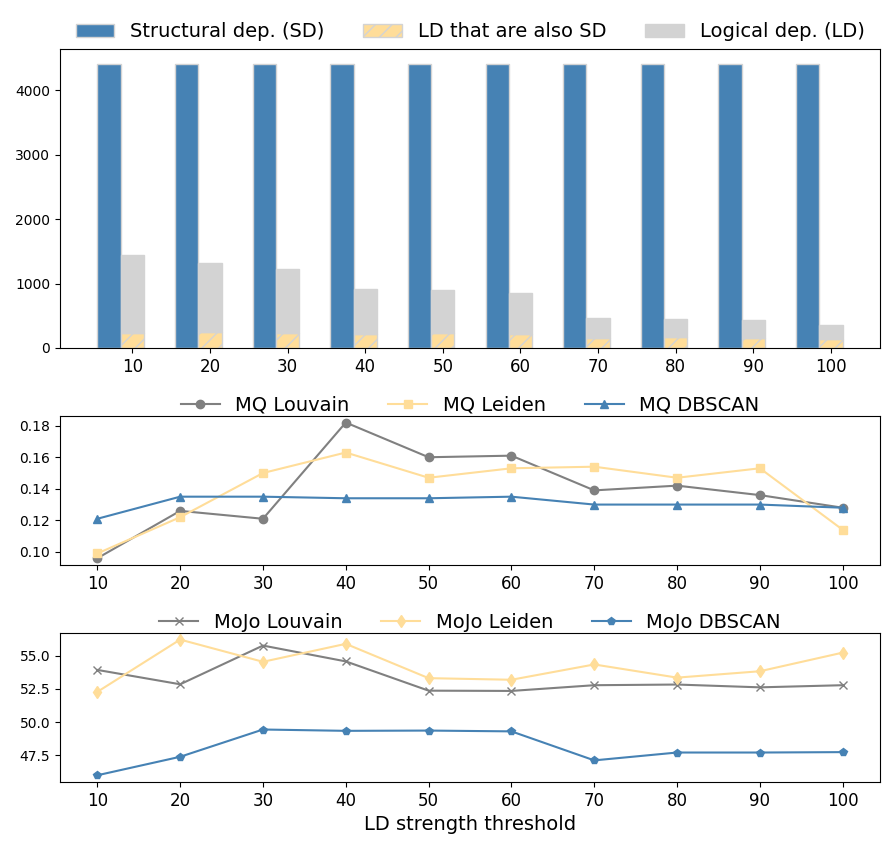
\includegraphics[width=\columnwidth]{hibernate_correlation.png}
  \caption{Hibernate ORM: Overlap between structural and logical dependencies and its correlation with clustering metrics.}
  \label{fig:hibernate_correlation}
\end{figure}

Hibernate has the lowest overlap percentage between LD and SD, as shown in Figure \ref{fig:hibernate_correlation}. Similar to the other systems, the performance for MQ and MoJoFM decreases for SD+LD as the strength threshold becomes stricter.

The results for Hibernate highlight the challenge of achieving better clustering in larger systems with fewer commits relative to their size.


\subsubsection{Google Gson}


\begin{figure}[t!]
  \centering
  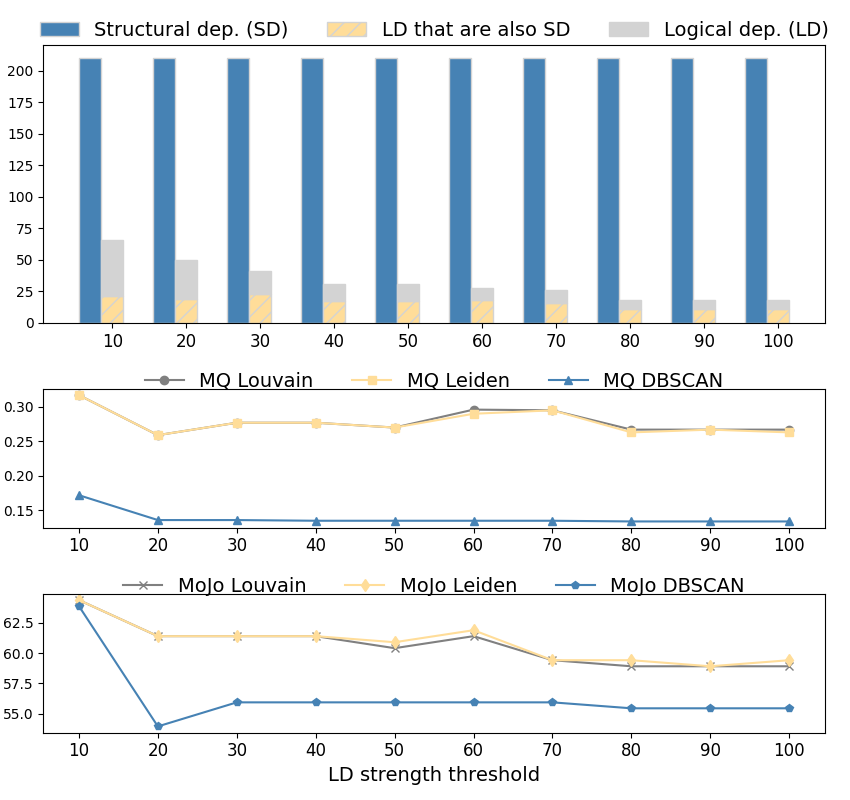
\includegraphics[width=\columnwidth]{gson_correlation.png}
  \caption{Google Gson: Overlap between structural and logical dependencies and its correlation with clustering metrics.}
  \label{fig:gson_correlation}
\end{figure}

Gson has the smallest number of commits analyzed, with 1,772 commits considered for LD extraction, and it is also the smallest in terms of system size, with 210 entities involved in clustering (Table \ref{tab:project_info}).

Based on the results from Table \ref{tab:clustering_results_gson}, the SD+LD combination with a strength threshold of 10 achieved the best results for both MQ and MoJoFM. Like Apache Ant and Tomcat, all SD+LD combinations achieve better MQ values than SD-only.

LD-only produced the best results for MQ at 40\% strength for both Louvain and Leiden, and the best MoJoFM value was also observed at the same threshold for both algorithms. It is the only system where the best MQ result for LD-only occurs at a lower strength threshold than 100\%. This is due to the very low number of entities remaining in the system at 100\% (only 18 out of 210).

In this particular system, it is more visible that the Leiden clustering algorithm does not improve the Louvain algorithm in some scenarios. This observation is based on the fact that the values obtained for both MQ and MoJoFM metrics are the same in most cases for the Gson system for both algorithms.

It can also be observed that Gson has identical metric values for MQ and MoJoFM across multiple strength thresholds. Again, the small number of commits and the size of the system contribute to the stability of these metrics.

Gson also has relatively high overlap rates between LD and SD compared to the other systems, as shown in Figure \ref{fig:gson_correlation}. Despite the constant values, the trend of decreasing performance for SD+LD with stricter strength filtering for LD is also present in Gson.

The results for this system highlight the difficulty of achieving better clustering solutions using logical dependencies in smaller systems with fewer commits. However, even for a small system like Gson, an improvement is still visible when using logical dependencies.

\subsection{Research Questions and Findings}

In this section, we will answer our research questions based on the results of our experiments. 

\textit{ \textbf{RQ1:} Does using structural dependencies (SD) combined with logical dependencies (LD) improve software clustering results compared to traditional approaches using only structural dependencies (SD)?} 

Based on the results from all four systems analyzed, the combination of SD and LD performed better than SD-only according to the MQ and MoJoFM metrics, confirming that using SD+LD improves software clustering results. Across different strength thresholds, SD+LD achieved higher MQ and MoJoFM values for all clustering algorithms, indicating better modularization. 
The filtering thresholds applied to logical dependencies influence the effectiveness of combining SD and LD. Lower strength thresholds (10\% to 40\%) resulted in better MQ and MoJoFM values across all clustering algorithms compared with higher thresholds.

At higher strength thresholds, the MQ and MoJoFM results decline. This decline occurs because stricter strength thresholds significantly reduce the amount of logical dependencies. This reduction leads to fewer new relationships introduced into the clustering process. Our previous research on the overlap between SD and LD showed that higher strength thresholds correlate with increased overlap between the two dependencies. This overlap indicates that at higher strength thresholds, not much new information is added to the system besides what is already introduced by structural dependencies, reducing the impact of logical dependencies on clustering results.

However, when considering a lower strength threshold, the relationship between the system size and the number of commits in the version history becomes an important factor.

In the case of Hibernate, a stricter strength threshold was needed to achieve the best metric values compared to other systems. Although the metrics obtained at a 10\% strength threshold for LD are better than SD-only, the system reached peak metric values at 40\% threshold across all algorithms.

With 16,609 commits and 4,414 entities, Hibernate has a significantly lower average number of commits per entity than Ant (14,917 commits and 517 entities) or Tomcat (22,698 commits and 662 entities). This lower ratio means that each entity in Hibernate is, on average, involved in fewer commits. As a result, the co-change data extracted for logical dependencies are sparser and contain more noise at lower strength thresholds.

A stricter strength threshold (e.g., 40\%) filters out these weaker logical dependencies.

In contrast, systems like Ant and Tomcat, with higher ratios of commits to entities, obtain better results with logical dependencies at a 10\% strength threshold because entities participate in more commits on average.

In conclusion, with an appropriate threshold, combining SD with LD leads to better clustering results than using SD alone.


\textit{\textbf{RQ2:} Can using only logical dependencies (LD) produce good software clustering results?} 

Using LD-only produced good clustering results, especially at higher strength thresholds. LD(100) produced the highest MQ and MoJoFM values for most systems compared with SD-only and SD+LD. However, the coverage of LD-only is significantly lower at these higher thresholds. For all systems, after filtering with 100\% strength threshold, the system coverage of the remaining logical dependencies is less than 17\% of the total known dependencies in the system.

Thus, while LD(100) provides the highest metric results compared to SD+LD and SD-only, it represents only a small subset of the system's dependencies.

On the other hand, LD(10) has, in most of the cases, better metric results than those for SD-only and SD+LD with better system coverage. Apache Ant and Tomcat LD(10) cover more than 60\% of the system, while for Hibernate and Gson, the coverage is slightly above 30\%. 

Therefore, LD(10) can be an alternative to SD-only or SD+LD, especially if structural dependencies are not available.

It is also important to consider that LD-only performance at higher strength thresholds depends on the system's characteristics, such as the number of commits and entities. For Gson project, the performance at a 100\% strength threshold is not as good as for the other systems, reaching its peak at a 40\% threshold. This is due to the low number of entities remaining at higher thresholds, with only 18 entities at the 80\% to 100\% strength thresholds, and the relatively small number of commits considered.

In summary, while LD-only can produce good clustering results, especially at higher strength thresholds, its limited coverage reduces its usability, as the clustering is intended for the entire system, not just a small subset. LD-only offers a good alternative to SD-only at lower strength thresholds, providing acceptable coverage.

\textit{ \textbf{RQ3:} How do different filtering settings for logical dependencies (LD) impact clustering results, and which filtering settings provide the best performance?}

The impact of different filtering settings on clustering performance was observed across all systems. For LD-only clustering, lower strength thresholds like 10\% provided good system coverage but had lower MQ and MoJoFM values compared to higher thresholds like 100\%, where the best metric results were often achieved. However, at these higher thresholds, the system coverage was significantly reduced.

The best performance was generally observed with strength thresholds between 10\% and 40\% for the combination of SD and LD (SD+LD). At these thresholds, the clustering solutions achieved higher MQ and MoJoFM values than SD alone.

It is important to select the optimal filtering threshold. Logical dependencies filtered with lower strength thresholds include more relationships, introducing more knowledge that could improve clustering results. However, a too-low threshold may sometimes introduce noise, especially in systems with a low commits-to-entities ratio. On the other hand, higher thresholds significantly reduce noise but can exclude valuable dependencies and decrease coverage.

The optimal filtering threshold may vary depending on system characteristics ( number of commits, size of the system), so it is important to consider these factors when filtering logical dependencies.


\section{Discussion on Ant clustering}
\label{discussion_ant}

Based on the results from Table \ref{tab:clustering-results2}, we can observe that the combined approach of structural dependencies and logical dependencies gives the highest Modularity Quality (MQ) metric of 0.227 with a strength threshold of 30\%, which is an improvement over the 0.08 MQ metric obtained when considering only structural dependencies.

Beyond the positive result indicated by the MQ metric, we searched for further validation by human software engineering expert opinion. After thoroughly studying and understanding the analyzed system source code and documentation, we evaluated the remodularization proposals resulting from the two clustering solutions.

The two clustering solutions compared are the clustering solution obtained only from structural dependencies, in comparison to the clustering solution obtained from using both structural and logical dependencies, filtered with a threshold of 30\% for strength.

The clustering solution relying solely on structural dependencies consists of 12 clusters, while the solution using both structural and logical dependencies consists of 15 clusters. Both solutions involve the same number of entities (517). The entities listed below are placed in different clusters:

\begin{itemize}
    \item taskdefs.Available\$FileDir
    \item taskdefs.Concat and its inner classes taskdefs.Concat\$1, taskdefs.Concat\$MultiReader, taskdefs.Concat\$ TextElement
    \item taskdefs.Javadoc\$AccessType
    \item util.WeakishReference and its inner class util.WeakishReference\$HardReference
    \item taskdefs.Replace and its inner classes taskdefs.Replace\$ NestedString, taskdefs.Replace\$Replacefilter
\end{itemize}

The migration of entities between clusters is illustrated in Figure \ref{fig:clustersmigration}. Given that the inner classes are shifted from one cluster to another in the same way as the outer class, we omitted the inner classes from the diagram.

As the cluster number itself is not significant and may vary across different script runs (labels might vary), we will refer to each individual cluster resulting from structural dependencies as \textit{Cluster A} and to the ones resulting from both logical and structural dependencies as \textit{Cluster B}.

\begin{figure}
\centering
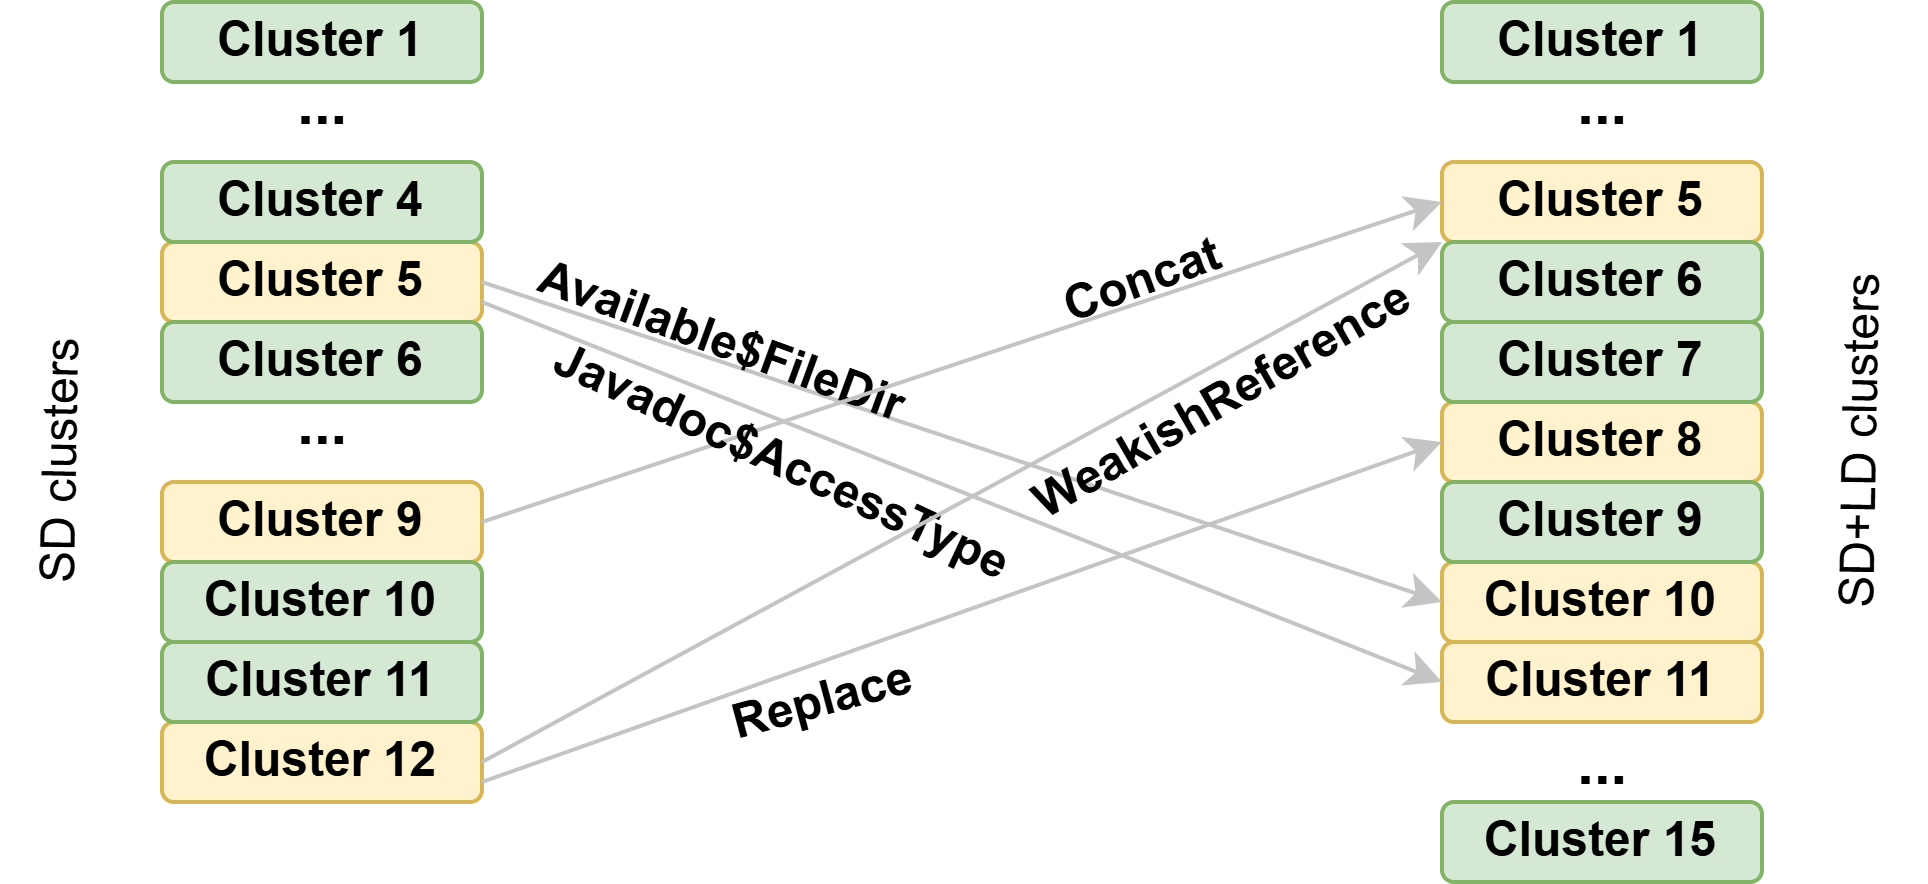
\includegraphics[width=\columnwidth]{clusters.png}
\caption{Migration of entities between clusters}
\label{fig:clustersmigration}
\centering
\end{figure}

\subsection{taskdefs.Concat and its inner classes}

To have a better overview of how and why entities are transferred between clusters, we depicted Concat's logical and structural connections in Figure \ref{fig:dep_concat}. Additionally, Figure \ref{fig:clusterAconcat} illustrates connections within Cluster A, while Figure \ref{fig:clusterBconcat} does the same for Cluster B.

In Cluster A, the Concat class and its inner classes (Concat\$1, Concat\$MultiReader, Concat\$TextElement) are placed together with conditions like Available, And, Or, IsTrue, Equals, IsReference, Contains.

On the other hand, in Cluster B, they are placed with classes associated with file manipulation and archive operations such as Ear, Jar, War, and Zip, as well as utility classes for file handling like FileUtils and JavaEnvUtils, and entities for zip file processing (ZipEntry, ZipFile). This placement is due to the logical dependencies that Concat class has with FileUtils and FileSet in the versioning system.

To assess whether the placement of Concat in Cluster B is better than in Cluster A, we referred to the official Ant documentation. According to the documentation: "This class contains the 'concat' task, used to concatenate a series of files into a single stream" \cite{ant_concat}. Therefore, judging by its usage and purpose according to the documentation, positioning the Concat class along with its inner classes in Cluster B is more suitable than in Cluster A.


\begin{figure}
\centering
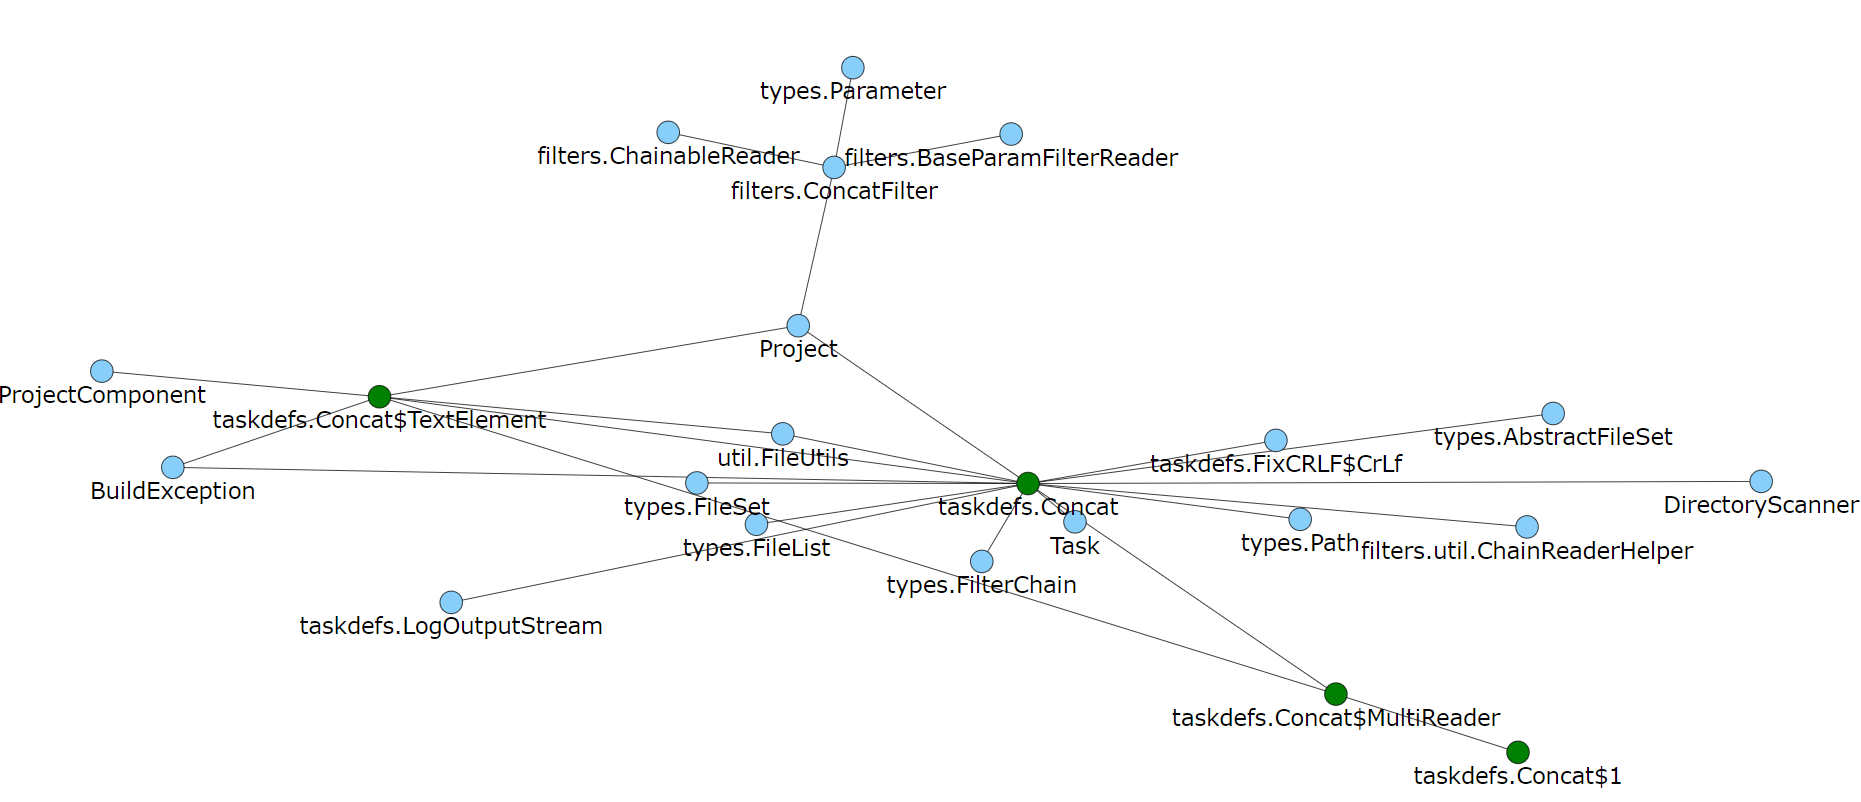
\includegraphics[width=\columnwidth]{dep_concat.png}
\caption{Dependencies (LD and SD) of Concat class}
\label{fig:dep_concat}
\centering
\end{figure}


\begin{figure}
\centering
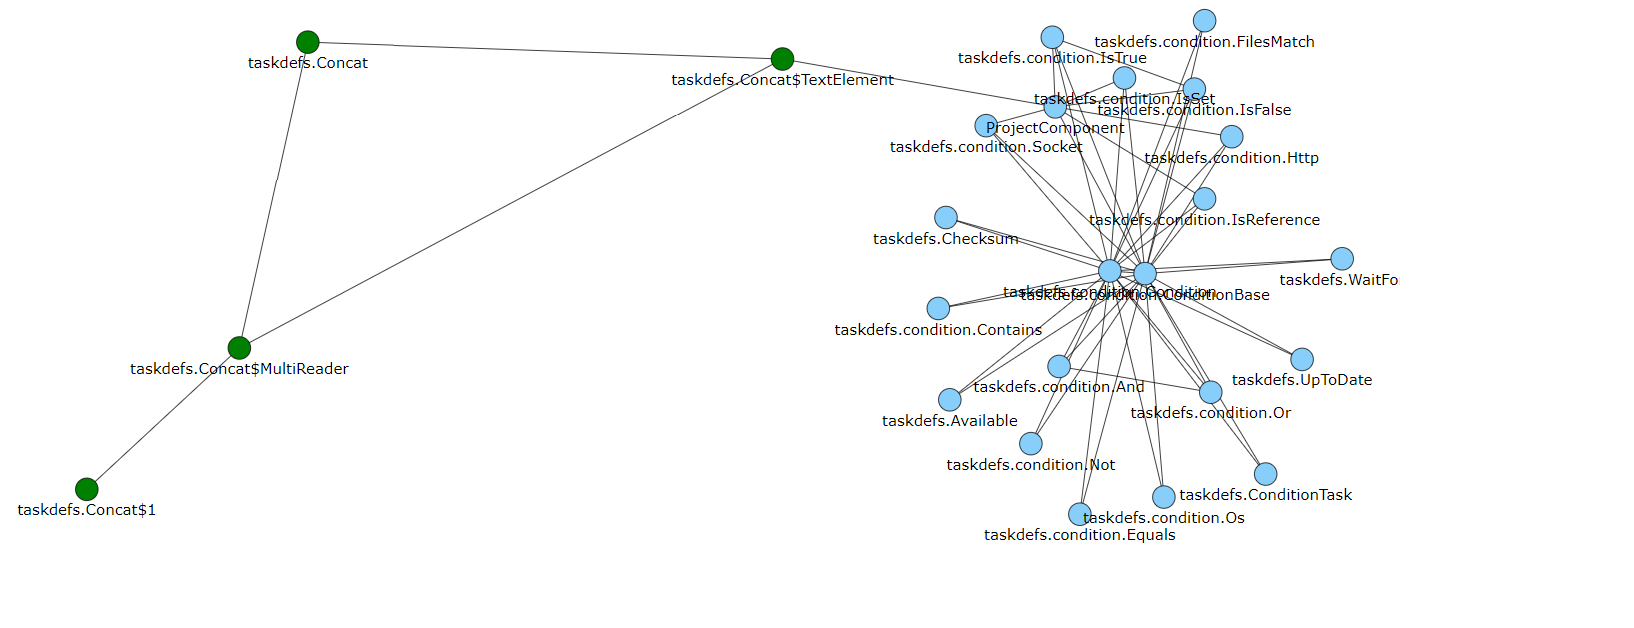
\includegraphics[width=\columnwidth]{cluster_concatSD.PNG}
\caption{Placement of Concat in ClusterA (SD); cluster size: 25}
\label{fig:clusterAconcat}
\centering
\end{figure}


\begin{figure}
\centering
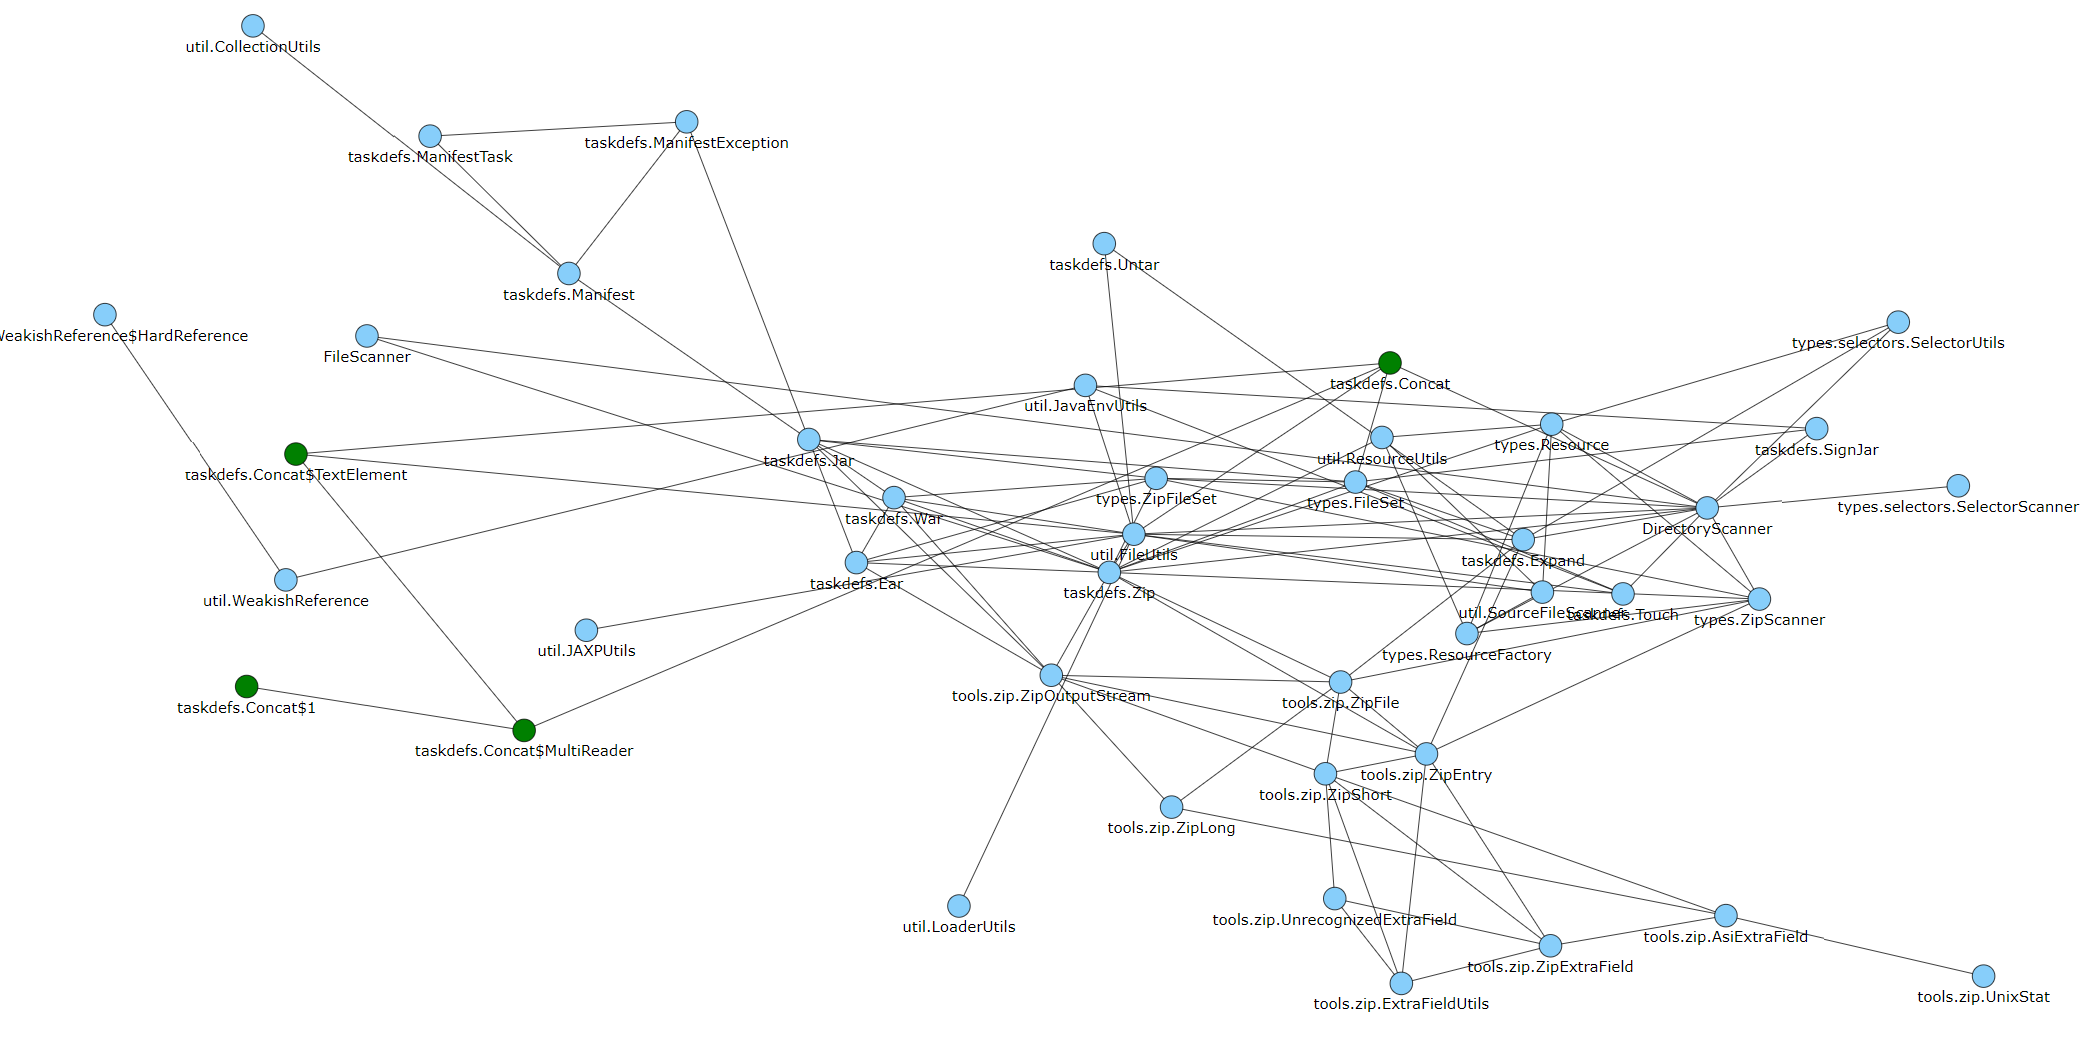
\includegraphics[width=\columnwidth]{cluster_concatSDLD.PNG}
\caption{Placement of Concat in ClusterB (SD and LD); cluster size: 52}
\label{fig:clusterBconcat}
\centering
\end{figure}

\subsection{taskdefs.Available\$FileDir}

In Cluster A the entity 'taskdefs.Available\$FileDir' is in the same cluster with entities that are related to the build process (ProjectHelper, TaskAdapter, ComponentHelper), but not with entities that have any relation to condition checks or file existence evaluations or with its outer class. 

Cluster B contains entities that are related to condition checking (And, Contains, Equals, Or, UpToDate), and also with the outer class of 'taskdefs.Available\$FileDir',  'taskdefs.Available'. The movement of entities from Cluster A to Cluster B was influenced by the logical dependencies between 'taskdefs.Available' and 'taskdefs.Available\$FileDir'.

The documentation description for 'taskdefs.Available' states: "Will set the given property if the requested resource is available at runtime. This task may also be used as a condition by the condition task."\cite{ant_concat}.
This reinforces its placement in Cluster B, which is centered around task definitions and conditions related to build processes.



\subsection{ taskdefs.Replace and its inner classes}

\begin{figure}
\centering
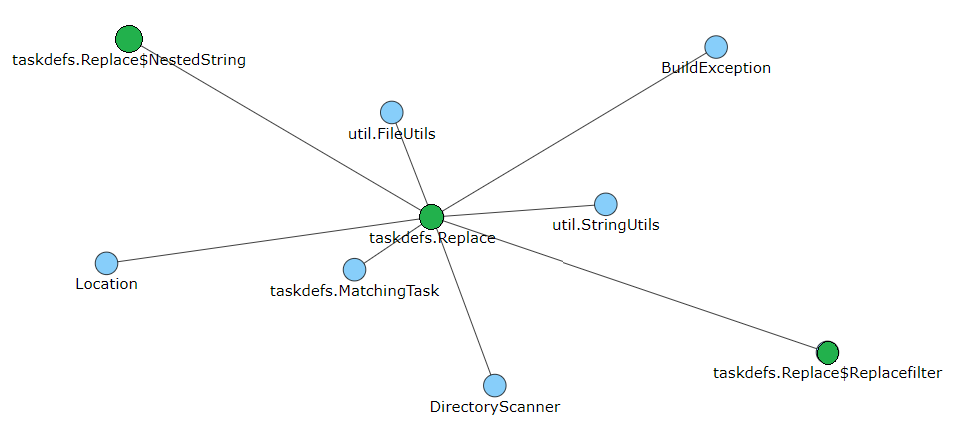
\includegraphics[width=\columnwidth]{dep_replace.png}
\caption{Ant dependencies (LD and SD) of Replace and its inner classes}
\label{fig:dep_replace}
\centering
\end{figure}

\begin{figure}
\centering
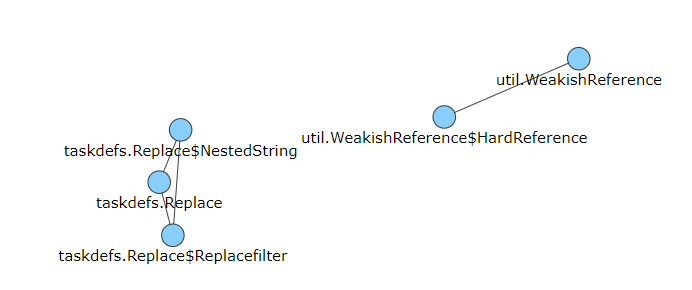
\includegraphics[width=\columnwidth]{cluster_replaceSD.PNG}
\caption{Placement of Replace in ClusterA (SD); cluster size: 5}
\label{fig:clusterAreplace}
\centering
\end{figure}


\begin{figure}
\centering
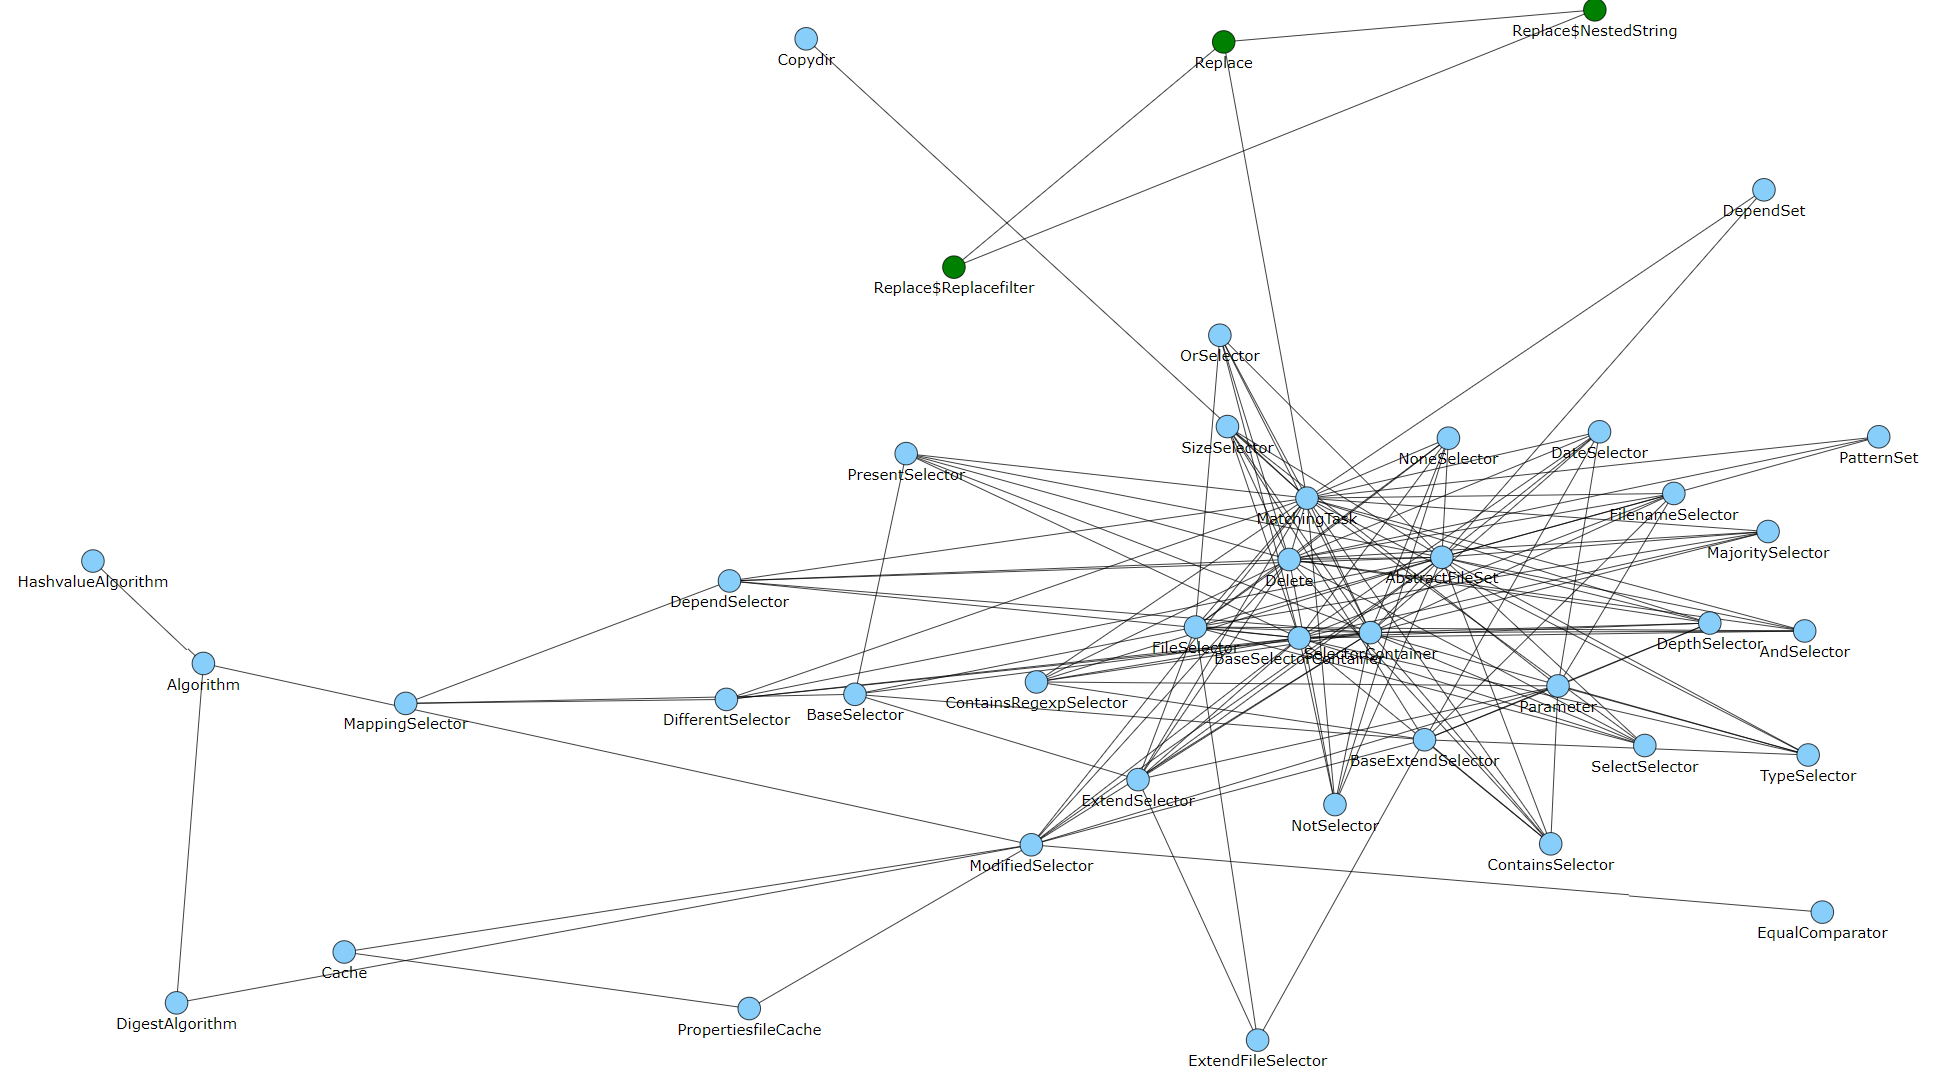
\includegraphics[width=\columnwidth]{cluster_replaceSDLD.PNG}
\caption{Placement of Replace in ClusterB (SD and LD); cluster size: 42}
\label{fig:clusterBreplace}
\centering
\end{figure}


We depicted the logical and structural connections of Replace in Figure \ref{fig:dep_replace}. Figure \ref{fig:clusterAreplace} illustrates connections within Cluster A, while Figure \ref{fig:clusterBreplace} does the same for Cluster B.

Replace and its inner classes are placed in Cluster B with entities with which they share common functionality and purpose, such as Copydir, Delete, DependSet, or MatchingTask. These entities are involved in similar tasks and operations. On the other hand, the placement in Cluster A, with WeakishReference and its inner class doesn't seem good, as these entities are completly unrelated.  

The movement of entities from Cluster A to Cluster B was influenced by the strong logical dependency between 'taskdefs.Replace' and 'taskdefs.MatchingTask'.

The cluster from figure \ref{fig:clusterAreplace} is the 12th cluster from the clustering solution based on structural dependencies. This particular cluster is essentially comprised of two unrelated entities: Replace and WeakishReference. Due to their logical dependencies, both entities are grouped within larger clusters that share similar functionalities in the SD and LD solution.




\newpage
\addcontentsline{toc}{section}{References}
\nocite{*}
\bibliographystyle{unsrt}
\bibliography{references}

\end{document}
